\documentclass[12pt,]{isuthesis}
\usepackage{lmodern}
\usepackage{amssymb,amsmath,mathptmx}
\usepackage{ifxetex,ifluatex}
\usepackage{fixltx2e} % provides \textsubscript
\ifnum 0\ifxetex 1\fi\ifluatex 1\fi=0 % if pdftex
  \usepackage[T1]{fontenc}
  \usepackage[utf8]{inputenc}
\else % if luatex or xelatex
  \ifxetex
    \usepackage{mathspec}
  \else
    \usepackage{fontspec}
  \fi
  \defaultfontfeatures{Ligatures=TeX,Scale=MatchLowercase}
\fi
% use upquote if available, for straight quotes in verbatim environments
\IfFileExists{upquote.sty}{\usepackage{upquote}}{}
% use microtype if available
\IfFileExists{microtype.sty}{%
\usepackage{microtype}
\UseMicrotypeSet[protrusion]{basicmath} % disable protrusion for tt fonts
}{}
\usepackage{hyperref}
\hypersetup{unicode=true,
            pdftitle={Interfacing R with Web Technologies for Data Acquistion and Interactive Visualization},
            pdfauthor={Carson Sievert},
            pdfborder={0 0 0},
            breaklinks=true}
\urlstyle{same}  % don't use monospace font for urls
\usepackage{color}
\usepackage{fancyvrb}
\newcommand{\VerbBar}{|}
\newcommand{\VERB}{\Verb[commandchars=\\\{\}]}
\DefineVerbatimEnvironment{Highlighting}{Verbatim}{commandchars=\\\{\}}
% Add ',fontsize=\small' for more characters per line
\usepackage{framed}
\definecolor{shadecolor}{RGB}{248,248,248}
\newenvironment{Shaded}{\begin{snugshade}}{\end{snugshade}}
\newcommand{\KeywordTok}[1]{\textcolor[rgb]{0.13,0.29,0.53}{\textbf{{#1}}}}
\newcommand{\DataTypeTok}[1]{\textcolor[rgb]{0.13,0.29,0.53}{{#1}}}
\newcommand{\DecValTok}[1]{\textcolor[rgb]{0.00,0.00,0.81}{{#1}}}
\newcommand{\BaseNTok}[1]{\textcolor[rgb]{0.00,0.00,0.81}{{#1}}}
\newcommand{\FloatTok}[1]{\textcolor[rgb]{0.00,0.00,0.81}{{#1}}}
\newcommand{\ConstantTok}[1]{\textcolor[rgb]{0.00,0.00,0.00}{{#1}}}
\newcommand{\CharTok}[1]{\textcolor[rgb]{0.31,0.60,0.02}{{#1}}}
\newcommand{\SpecialCharTok}[1]{\textcolor[rgb]{0.00,0.00,0.00}{{#1}}}
\newcommand{\StringTok}[1]{\textcolor[rgb]{0.31,0.60,0.02}{{#1}}}
\newcommand{\VerbatimStringTok}[1]{\textcolor[rgb]{0.31,0.60,0.02}{{#1}}}
\newcommand{\SpecialStringTok}[1]{\textcolor[rgb]{0.31,0.60,0.02}{{#1}}}
\newcommand{\ImportTok}[1]{{#1}}
\newcommand{\CommentTok}[1]{\textcolor[rgb]{0.56,0.35,0.01}{\textit{{#1}}}}
\newcommand{\DocumentationTok}[1]{\textcolor[rgb]{0.56,0.35,0.01}{\textbf{\textit{{#1}}}}}
\newcommand{\AnnotationTok}[1]{\textcolor[rgb]{0.56,0.35,0.01}{\textbf{\textit{{#1}}}}}
\newcommand{\CommentVarTok}[1]{\textcolor[rgb]{0.56,0.35,0.01}{\textbf{\textit{{#1}}}}}
\newcommand{\OtherTok}[1]{\textcolor[rgb]{0.56,0.35,0.01}{{#1}}}
\newcommand{\FunctionTok}[1]{\textcolor[rgb]{0.00,0.00,0.00}{{#1}}}
\newcommand{\VariableTok}[1]{\textcolor[rgb]{0.00,0.00,0.00}{{#1}}}
\newcommand{\ControlFlowTok}[1]{\textcolor[rgb]{0.13,0.29,0.53}{\textbf{{#1}}}}
\newcommand{\OperatorTok}[1]{\textcolor[rgb]{0.81,0.36,0.00}{\textbf{{#1}}}}
\newcommand{\BuiltInTok}[1]{{#1}}
\newcommand{\ExtensionTok}[1]{{#1}}
\newcommand{\PreprocessorTok}[1]{\textcolor[rgb]{0.56,0.35,0.01}{\textit{{#1}}}}
\newcommand{\AttributeTok}[1]{\textcolor[rgb]{0.77,0.63,0.00}{{#1}}}
\newcommand{\RegionMarkerTok}[1]{{#1}}
\newcommand{\InformationTok}[1]{\textcolor[rgb]{0.56,0.35,0.01}{\textbf{\textit{{#1}}}}}
\newcommand{\WarningTok}[1]{\textcolor[rgb]{0.56,0.35,0.01}{\textbf{\textit{{#1}}}}}
\newcommand{\AlertTok}[1]{\textcolor[rgb]{0.94,0.16,0.16}{{#1}}}
\newcommand{\ErrorTok}[1]{\textcolor[rgb]{0.64,0.00,0.00}{\textbf{{#1}}}}
\newcommand{\NormalTok}[1]{{#1}}
\usepackage{longtable,booktabs,widetable}

% always, graphics silly
\usepackage{graphicx,grffile}
\makeatletter
\def\maxwidth{\ifdim\Gin@nat@width>\linewidth\linewidth\else\Gin@nat@width\fi}
\def\maxheight{\ifdim\Gin@nat@height>\textheight\textheight\else\Gin@nat@height\fi}
\makeatother
% Scale images if necessary, so that they will not overflow the page
% margins by default, and it is still possible to overwrite the defaults
% using explicit options in \includegraphics[width, height, ...]{}
\setkeys{Gin}{width=\maxwidth,height=\maxheight,keepaspectratio}


\IfFileExists{parskip.sty}{%
\usepackage{parskip}
}{% else
\setlength{\parindent}{0pt}
\setlength{\parskip}{6pt plus 2pt minus 1pt}
}
\setlength{\emergencystretch}{3em}  % prevent overfull lines
\providecommand{\tightlist}{%
  \setlength{\itemsep}{0pt}\setlength{\parskip}{0pt}}
\setcounter{secnumdepth}{5}
% Redefines (sub)paragraphs to behave more like sections
\ifx\paragraph\undefined\else
\let\oldparagraph\paragraph
\renewcommand{\paragraph}[1]{\oldparagraph{#1}\mbox{}}
\fi
\ifx\subparagraph\undefined\else
\let\oldsubparagraph\subparagraph
\renewcommand{\subparagraph}[1]{\oldsubparagraph{#1}\mbox{}}
\fi

%%% Use protect on footnotes to avoid problems with footnotes in titles
\let\rmarkdownfootnote\footnote%
\def\footnote{\protect\rmarkdownfootnote}

%%% Change title format to be more compact
\usepackage{titling}

% Create subtitle command for use in maketitle
\newcommand{\subtitle}[1]{
 \posttitle{
   \begin{center}\large#1\end{center}
   }
}

\setlength{\droptitle}{-2em}
 \title{Interfacing R with Web Technologies for Data Acquistion and Interactive
Visualization}
 \pretitle{\vspace{\droptitle}\centering\huge}
 \posttitle{\par}
 \author{Carson Sievert}
 \preauthor{\centering\large\emph}
 \postauthor{\par}
 \date{}
 \predate{}\postdate{}



\begin{document}

\maketitle

{
\setcounter{tocdepth}{2}
\tableofcontents
}
\addcontentsline{toc}{chapter}{LIST OF TABLES}
\listoftables
\cleardoublepage \phantomsection \addcontentsline{toc}{chapter}{LIST OF FIGURES}
\listoffigures

\cleardoublepage \phantomsection
\specialchapt{ACKNOWLEDGEMENTS}

This thesis would not be possible without many people. First and foremost, special thanks to my major professor Heike Hofmann. I would not made it to this point without such a warm and friendly mentor who was often more confident in my abilities than I was of my own. Thank you for always supporting me no matter how many things I had going on to distract me from research. I aspire to inherit the same empathy and support that you show to your students on a daily basis. 

Another special thanks goes to Di Cook. In the fourth year of my PhD, I was experiencing burnout (and growing tired of Ames), when Di took me to lunch, told me she was transferring to Monash University in Australia, and invited me to join her. Of course, I said yes, and when I arrived, I immediately felt welcomed and a part of the group -- all thanks to Di. She strategically assigned me to assist her students with their thesis projects, run R workshops for the university, and most importantly, work on my tennis game. Through this "work" I met so many amazing people and had many memorable experiences. Those 6 months gave me a new perspective on life in general and I am forever grateful for being blessed enough to take the opportunity.

Thank you to many of Heike and Di's former students who came before me (just to name a few: Hadley Wickham, Michael Lawrence, Yihui Xie, Xiaoyue Cheng, Barrett Schloerke, Susan VanderPlas). Your work has not only inspired and enabled my work, but it has also enabled an entire community of people working with data to do amazing things. Without this strong history and community at Iowa State, I would not have had the courage or the vision to follow such a "non-traditional" research path. I hope the University continues to value this type of work as it teaches students skills that are in high demand and generally improves the way data-driven research is performed.

Thank you to all my collaborators, especially Toby Dylan Hocking. Toby and Susan VanderPlas laid the initial framework for \textbf{animint} -- which I first worked on as a Google Summer of Code student under Toby's guidance. Toby later went on write the initial version of the \texttt{ggplotly}() function in \textbf{plotly}, borrowing a lot of ideas from \textbf{animint}. As Toby became busy with other things, he introduced me to the plotly team, and eventually handed over the reigns on the project, which has helped to financially support the last year or so of grad school.

Thank you also to the plotly team, and in particular, the software engineers who work on the open source project plotly.js. My work has benefited greatly from your responsiveness to my questions, feature requests, and bug reports. I have a great amount of respect for the work that you do, and I hope this project keeps improving at its current break neck pace.

Finally, thank you to my family for their encouragement and keeping me grounded throughout this experience. Thank you to my father for the initial encouragement to pursue a PhD, conversations surrounding work-life balance, and also pushing me to "graduate before I'm 40". Thank you to my mother for her unconditional love, endless care, and predenting to understand what I do for a living. Thank you to my brothers for providing me with shelter, beer, and Twins tickets. Thank you all for your willingness to drop everything to help me at any given moment. I can't say I've always been as willing, as I have been selfish with my time during my PhD, but I hope to change that after graduation.


\newpage
\pagenumbering{arabic}
\chapter{Literature Review}

\section{What makes a good software
interface?}\label{what-makes-a-good-software-interface}

Unwin and Hofmann (Unwin and Hofmann
\protect\hyperlink{ref-Unwin:1999vp}{2009}) discuss the strengths,
weaknesses, and differences between using graphical and command-line
interfaces for data analysis. Graphical user interfaces (GUIs) can be
much more intuitive to use, but at the cost of being less flexible,
precise, and repeatable. Unwin and Hofmann argue statistical software
should strive to achieve a synergy of two that leverages both of their
strengths. That is, a command-line interface when we can precisely
describe what we want and a graphical interface for ``searching for
information and interesting structures without fully specified
questions.''

Unwin and Hofmann further discuss the different audiences these
interfaces attract. Command-line interfaces typically attract ``power
users'' such as applied statisticians and statistical researchers in a
university, whereas more casual users of statistical software typically
prefer a GUI. In later sections, we discuss GUIs in greater detail
within the context of interactive statistical graphics. For now, we
briefly discuss some best practices for designing a command-line
interface for statistical computing in R.

Before authoring an interface, one should establish the target audience,
the class of problems it should address, and loosely define how the
interface should actually work. During this process, it may also be
helpful to identify your audience as being primarily composed of
\emph{software developers} or \emph{data analysts}. Developers are
typically more interested in using the interface to develop novel
software or incorporating the functionality into a larger scientific
computing environment (Jereon Ooms
\protect\hyperlink{ref-embedded-computing}{2014}). In this case,
interactive exploration and troubleshooting is not always a luxury, so
robust functionality is of utmost importance. On the other hand,
analysts interfaces should work well in an interactive environment since
this caters to rapid prototyping of ideas and troubleshooting of errors.

Good developer interfaces often make it easier to implement good analyst
interfaces. A great recent example of a good developer interface is the
R package \textbf{Rcpp}, which provides a seamless interface between R
with C++ (Eddelbuettel \protect\hyperlink{ref-Rcpp}{2013}). To date,
more than 500 R packages use \textbf{Rcpp} to make interfaces that are
both expressive and efficient, including the highly influential analyst
interfaces such as \textbf{tidyr} and \textbf{dplyr} (Wickham
\protect\hyperlink{ref-tidy-data}{2014}); (Wickham and Francois
\protect\hyperlink{ref-dplyr}{2014}). These interfaces help analysts
focus on the primary task of wrangling data into a form suitable for
visualization and statistical modeling, rather than focusing on the
implementation details behind how the transformations are performed.
(Donoho \protect\hyperlink{ref-Donoho:2015tu}{2015}) argues that these
interfaces ``May have more impact on today's practice of data analysis
than many highly-regarded theoretical statistics papers''.

Evaluating statistical computing interfaces is certainly a subjective
matter since we all have different tastes, different backgrounds, and
have different needs. It seems reasonable to evaluate an interface based
on its effectiveness and efficiency in aiding a user complete their
task, but as (Unwin and Hofmann
\protect\hyperlink{ref-Unwin:1999vp}{2009}) points out, ``There is a
tendency to judge software by the most powerful tools they provide
(whether with a good interface or not)''. As a result, all too often,
analysts must spend time gaining the skills of a software developer.
Good analyst interfaces often abstract functionality from developer
interfaces in a way that allow analysts to focus on their primary task
of acquiring/analyzing/modeling/visualizing data, rather than the
implementation details. The following focuses on such work with respect
to acquiring data from the web and interactive statistical web graphics.

\section{Acquiring and wrangling web content in
R}\label{acquiring-and-wrangling-web-content-in-r}

\subsection{Interfaces for working with web
content}\label{interfaces-for-working-with-web-content}

R has a rich history of interfacing with web technologies for
accomplishing a variety of tasks such as requesting, manipulating, and
creating web content. As an important first step, extending ideas from
(Chambers \protect\hyperlink{ref-Chambers:1999}{1999}), Brian Ripley
implemented the connections interface for file-oriented input/output in
R (Ripley \protect\hyperlink{ref-Connections}{2001}). This interface
supports a variety of common transfer protocols (HTTP, HTTPS, FTP),
providing access to most files on the web that can be identified with a
Uniform Resource Locator (URL). Connection objects are actually external
pointers, meaning that, instead of immediately reading the file, they
just point to the file, and make no assumptions about the actual
contents of the file.

Many functions in the base R distribution for reading data (e.g.,
\texttt{scan}, \texttt{read.table}, \texttt{read.csv}, etc.) are built
on top of connections, and provide additional functionality for parsing
well-structured plain-text into basic R data structures (vector, list,
data frame, etc.). However, the base R distribution does not provide
functionality for parsing common file formats found on the web (e.g.,
HTML, XML, JSON). In addition, the standard R connection interface
provides no support for communicating with web servers beyond a simple
HTTP GET request (Lang \protect\hyperlink{ref-Lang:2006us}{2006}).

The \textbf{RCurl}, \textbf{XML}, and \textbf{RJSONIO} packages were
major contributions that drastically improved our ability to request,
manipulate, and create web content from R (Nolan and Temple Lang
\protect\hyperlink{ref-nolan-lang}{2014}). The \textbf{RCurl} package
provides a suite of high and low level bindings to the C library
libcurl, making it possible to transfer files over more network
protocols, communicate with web servers (e.g., submit forms, upload
files, etc.), process their responses, and handle other details such as
redirects and authentication (Temple Lang
\protect\hyperlink{ref-RCurl}{2014}\protect\hyperlink{ref-RCurl}{a}).
The \textbf{XML} package provides low-level bindings to the C library
libxml2, making it possible to download, parse, manipulate, and create
XML (and HTML) (Lang \protect\hyperlink{ref-XML}{2013}). To make this
possible, \textbf{XML} also provides some data structures for
representing XML in R. The \textbf{RJSONIO} package provides a mapping
between R objects and JavaScript Object Notation (JSON) (Temple Lang
\protect\hyperlink{ref-RJSONIO}{2014}\protect\hyperlink{ref-RJSONIO}{b}).
These packages were heavily used for years, but several newer interfaces
have made these tasks easier and more efficient.

The \textbf{curl}, \textbf{httr}, and \textbf{jsonlite} packages are
more modern R interfaces for requesting content on the web and
interacting with web servers. The \textbf{curl} package provides a much
simpler interface to libcurl that also supports streaming data (useful
for transferring large data), and generally has better performance than
\textbf{RCurl} (Ooms \protect\hyperlink{ref-curl}{2015}). The
\textbf{httr} package builds on \textbf{curl} and organizes it's
functionality around HTTP verbs (GET, POST, etc.) (Wickham
\protect\hyperlink{ref-httr}{2015}\protect\hyperlink{ref-httr}{a}).
Since most web application programming interfaces (APIs) organize their
functionality around these same verbs, it is often very easy to write R
bindings to web services with \textbf{httr}. The \textbf{httr} package
also builds on \textbf{jsonlite} since it provides consistent mappings
between R/JSON and most most modern web APIs accept and send messages in
JSON format (Jeroen Ooms
\protect\hyperlink{ref-jsonlite}{2014}\protect\hyperlink{ref-jsonlite}{a}).
These packages have already had a profound impact on the investment
required to interface R with web services, which are useful for many
things beyond data acquisition. For example, it is now easy to install R
packages hosted on the web (\textbf{devtools}), perform cloud computing
(\textbf{analogsea}), and archive/share computational outputs
(\textbf{dvn}, \textbf{rfigshare}, \textbf{RAmazonS3},
\textbf{googlesheets}, \textbf{rdrop2}, etc.).

The \textbf{rvest} package builds on \textbf{httr} and makes it easy to
manipulate content in HTML/XML files (Wickham
\protect\hyperlink{ref-rvest}{2015}\protect\hyperlink{ref-rvest}{c}).
Using \textbf{rvest} in combination with
\href{http://selectorgadget.com/}{SelectorGadget}, it is often possible
to extract structured information (e.g., tables, lists, links, etc) from
HTML with almost no knowledge/familiarity with web technologies. The
\textbf{XML2R} package has a similar goal of providing an interface to
acquire and manipulate XML content into tabular R data structures
without any working knowledge of XML/XSLT/XPath (Sievert
\protect\hyperlink{ref-Sievert:2014a}{2014}\protect\hyperlink{ref-Sievert:2014a}{b}).
As a result, these interfaces reduce the startup costs required for
analysts to acquire data from the web.

Packages such as \textbf{XML}, \textbf{XML2R}, and \textbf{rvest} can
download and parse the source of web pages, which is \emph{static}, but
extracting \emph{dynamic} web content requires additional tools. The R
package \textbf{rdom} fills this void and makes it easy to render and
access the Document Object Model (DOM) using the headless browsing
engine phantomjs (Sievert
\protect\hyperlink{ref-rdom}{2015}\protect\hyperlink{ref-rdom}{a}). The
R package \textbf{RSelenium} can also render dynamic web pages and
simulate user actions, but its broad scope and heavy software
requirements make it harder to use and less reliable compared to
\textbf{rdom} (Harrison \protect\hyperlink{ref-RSelenium}{2014}).
\textbf{rdom} is also designed to work seamlessly with \textbf{rvest},
so that one may use the \texttt{rdom()} function instead of
\texttt{read\_html()} to render, parse, and return the DOM as HTML
(instead of just the HTML page source).

Any combination of these R packages may be useful in acquiring data for
personal use and/or providing a higher-level interface to specific data
source(s) to increase their accessibility. The next section focuses on
such interfaces.

\subsection{Interfaces for acquiring data on the
web}\label{interfaces-for-acquiring-data-on-the-web}

The web provides access to the world's largest repository of publicly
available information and data. This provides a nice \emph{potential}
resource both teaching and practicing applied statistics, but to be
practical useful, it often requires a custom interface to make data more
accessible. If publishers follow best practices, a custom interface to
the data source usually is not needed, but this is rarely the case. Many
times structured data is embedded within larger unstructured documents,
making it difficult to incorporate into a data analysis workflow. This
is especially true of data used to inform downstream web applications,
typically in XML and/or JSON format. There are two main ways to make
such data more accessible: (1) package, document, and distribute the
data itself (2) provide functionality to acquire the data.

If the data source is fairly small, somewhat static, and freely
available with an open license, then we can directly provide data via R
packaging mechanism. In this case, it is best practice for package
authors include scripts used to acquire, transform, and clean the data.
This model is especially nice for both teaching and providing examples,
since users can easily access data by installing the R package. (Wickham
\protect\hyperlink{ref-rpkgs}{2015}\protect\hyperlink{ref-rpkgs}{b})
provides a nice section outlining the details of bundling data with R
packages.\footnote{This section is freely available online
  \url{http://r-pkgs.had.co.nz/data.html}.}

R packages that just provide functionality to acquire data can be more
desirable than bundling it for several reasons. In some cases, it helps
avoid legal issues with rehosting copyrighted data. Furthermore, the
source code of R packages can always be inspected, so users can verify
the cleaning and transformations performed on the data to ensure its
integrity, and suggest changes if necessary. They are also versioned,
which makes the data acquisition, and thus any downstream analysis, more
reproducible and transparent. It is also possible to handle dynamic data
with such interfaces, meaning that new data can be acquired without any
change to the underlying source code. As explained in
\protect\hyperlink{taming-pitchfx-data-with-xml2r-and-pitchrx}{Taming
PITCHf/x Data with XML2R and pitchRx}, this is an important quality of
the \textbf{pitchRx} R package since new PITCHf/x data is made available
on a daily basis.

Perhaps the largest centralized effort in this domain is lead by
\href{https://ropensci.org}{rOpenSci}, a community of R developers that,
at the time of writing, maintains more than 50 packages providing access
to scientific data ranging from bird sightings, species occurrence, and
even text/metadata from academic publications. This provides a
tremendous service to researchers who want to spend their time building
models and deriving insights from data, rather than learning the
programming skills necessary to acquire and clean it.

It's becoming increasingly clear that ``meta'' packages that standardize
the interface to data acquisition/curation in a particular domain would
be tremendously useful. However, it is not clear how such interfaces
should be designed. The R package \textbf{etl} is one step in this
direction and aims to provide a standardized interface for \emph{any}
data access package that fits into an Extract-Transform-Load paradigm
(Baumer and Sievert \protect\hyperlink{ref-etl}{2016}). The package
provides generic \texttt{extract}-\texttt{transform}-\texttt{load}
functions, but requires package authors to write custom
\texttt{extract}-\texttt{transform} methods for the specific data
source. In theory, the default \texttt{load} method works for any
application; as well as other database management operations such as
\texttt{update} and \texttt{clean}.

\section{Dynamic interactive statistical web
graphics}\label{dynamic-interactive-statistical-web-graphics}

\subsection{Why interactive?}\label{why-interactive}

Unlike computer graphics which focuses on representing reality,
virtually; data visualization is about garnering abstract relationships
between multiple variables from visual representation. The
dimensionality of data, the number of variables can be anything, usually
more than 3D, which summons a need to get beyond 2D canvasses for
display. Technology enables this, enabling the user to see many views,
query and link components. As demonstrated in Figure \ref{fig:touR}
using the R package \textbf{tourbrush} (Sievert
\protect\hyperlink{ref-tourbrush}{2015}\protect\hyperlink{ref-tourbrush}{b}),
interactive and dynamic graphics allow us to go beyond the constraints
of low-dimensional displays to see high-dimensional relationships in
data.

\begin{figure}[htbp]
\centering
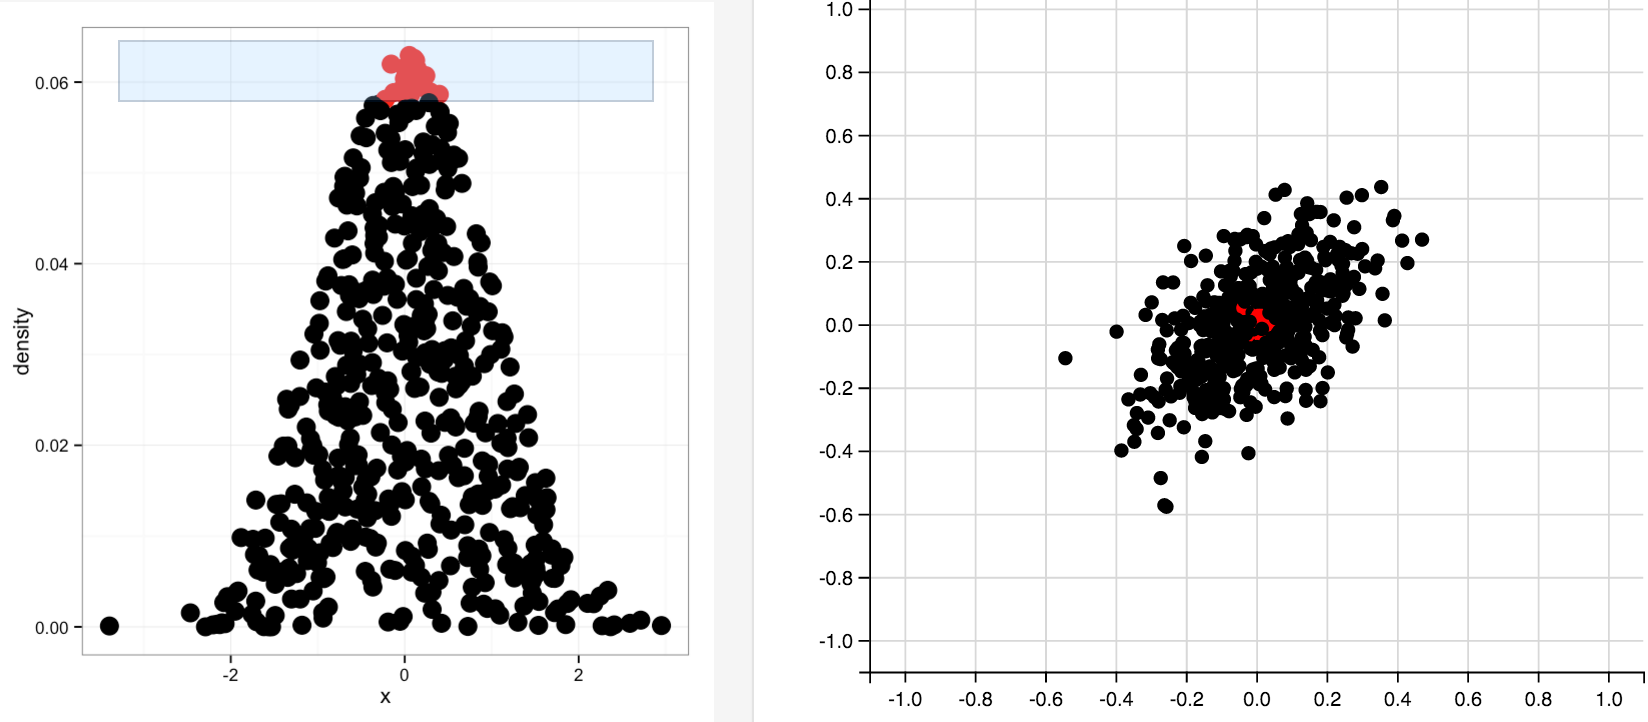
\includegraphics{images/tourbrush}
\caption{\label{fig:touR}A demonstration of interactive and dynamic
techniques for visualizing high-dimensional relationships in data using
the R package \textbf{tourbrush}. You can view this movie online at
\url{https://vimeo.com/148050343} or via the supplementary materials}
\end{figure}

Dynamic interactive statistical graphics is useful for descriptive
statistics, and also to help build better inferential models. Any
statistician is familiar with diagnosing a model by plotting data in the
model space (e.g., residual plot, qqplot). This works well for
determining if the assumptions of a model are adequate, but rarely
suggests that our model neglects important features in the data. To
combat this problem, Wickham, Cook, and Hofmann
(\protect\hyperlink{ref-Wickham:2015ur}{2015}) suggest to plot the model
in the data space and use dynamic interactive statistical graphics to do
so. Interactive graphics have also proved to be useful for exploratory
model analysis, a situation where we have many models to evaluate,
compare, and critique (Unwin, Volinsky, and Winkler
\protect\hyperlink{ref-Unwin:2003uy}{2003}); (Urbanek
\protect\hyperlink{ref-Urbanek:2004}{2004}); (Ripley
\protect\hyperlink{ref-Ripley:2004}{2004}); (Unwin
\protect\hyperlink{ref-Unwin:2006}{2006}); (Wickham
\protect\hyperlink{ref-Wickham:2007wq}{2007}). With such power comes
responsibility that we can verify that visual discoveries are real, and
not due to random chance (Buja et al.
\protect\hyperlink{ref-Buja:2009hp}{2009}); (Majumder, Hofmann, and Cook
\protect\hyperlink{ref-Majumder:2013ie}{2013}).

The ASA Section on Statistical Computing and Graphics maintains a video
library which captures many useful dynamic interactive statistical
graphics techniques. Several videos show how XGobi (predecessor to
GGobi), a dynamic interactive statistical graphics system, can be used
to reveal high-dimensional relationships and structures that cannot be
easily identified using numerical methods alone (Swayne, Cook, and Buja
\protect\hyperlink{ref-xgobi}{1998}).\footnote{For example,
  \url{http://stat-graphics.org/movies/xgobi.html} and
  \url{http://stat-graphics.org/movies/grand-tour.html}} Another notable
video shows how the interactive graphics system mondrian can be used to
quickly find interesting patterns in high-dimensional data using
exploratory data analysis (EDA) techniques (Theus and Urbanek
\protect\hyperlink{ref-mondrianbook}{2008}).\footnote{\url{http://stat-graphics.org/movies/tour-de-france.html}}
The most recent video shows how dynamic interactive techniques can help
interpret a topic model (a statistical mixture model applied to text
data) using the R package \textbf{LDAvis} (Sievert and Shirley
\protect\hyperlink{ref-Sievert:2014b}{2014}), which is the first
web-based visualization in the library, and is discussed at depth in
\protect\hyperlink{ldavis-a-method-for-visualizing-and-interpreting-topics}{LDAvis:
A method for visualizing and interpreting topics}.

In order to be practically useful, interactive statistical graphics must
be fast, flexible, accessible, portable, and reproducible. In general,
over the last 20-30 years interactive graphics systems were fast and
flexible, but were generally not easily accessible, portable, or
reproducible. The web browser provides a convenient platform to combat
these problems. For example, any visualization created with
\textbf{LDAvis} can be shared through a Uniform Resource Locator (URL),
meaning that anyone with a web browser and an internet connection can
view and interact with a visualization. Furthermore, we can link anyone
to any possible state of the visualization by encoding selections with a
URL fragment identifier. This makes it possible to link readers to an
interesting state of a visualization from an external document, while
still allowing them to independently explore the same visualization and
assess conclusions drawn from it.\footnote{A good example of is
  \url{http://cpsievert.github.io/LDAvis/reviews/reviews.html}}

\subsection{Indirect versus direct
manipulation}\label{indirect-versus-direct-manipulation}

Even within the statistical graphics community, the term
\emph{interactive} graphics can mean wildly different things to
different people (Swayne and Klinke
\protect\hyperlink{ref-swayne-klinke}{1999}). Some early statistical
literature on the topic uses interactive in the sense that an
interactive command-line prompt allows users to create graphics
on-the-fly (R. A. Becker \protect\hyperlink{ref-S:1984}{1984}). That is,
users enter commands into the command-line prompt, the prompts evaluates
the command, and prints the result (known as the read--eval--print loop
(REPL)). Modifying a command to generate another variation of a
particular result (e.g., to restyle a static plot) can be thought of as
a type of interaction that some might call \emph{indirect manipulation}.

Indirect manipulation can be achieved both from the command-line or from
a graphical user interface (GUI). Indirect manipulation from the
command-line is more flexible since we have complete control over the
commands, but it is also more cumbersome since we must translate our
thoughts into code. Indirect manipulation via a GUI is more restrictive,
but it helps reduces the gulf of execution (i.e., easier to generate
desired output) for end-users (Hutchins, Hollan, and Norman
\protect\hyperlink{ref-Hutchins:1985wu}{1985}). In this sense, a GUI can
be useful, even for experienced programmers, when the command-line
interface impedes our primary task of deriving insight from data.

In many cases, the gulf of execution can be further reduced through
direct manipulation. Roughly speaking, within the context of interactive
graphics, direct manipulation occurs whenever we interact with a plot
and reveal new information tied to the event. Cook and Swayne
(\protect\hyperlink{ref-ggobi:2007}{2007}) use the terms dynamic
graphics and direct manipulation to characterize ``plots that respond in
real time to an analyst's queries and change dynamically to re-focus,
link to information from other sources, and re-organize information.''
Directly manipulating multiple linked views to make graphical queries is
a very powerful framework for exploring information, and inspires the
last 3 chapters of this thesis.

A simple example to help demonstrate the differences between these
interactive techniques would be in an analysis of variance (ANOVA) via
multiple boxplots. By default, most plotting libraries sort categories
alphabetically, but this is usually not optimal for visual comparison of
groups. With a static plotting library such as \textbf{ggplot2}, we
could indirectly manipulate the default by going back to the
command-line, reordering the factor levels of the categorical variables,
and regenerate the plot (Wickham
\protect\hyperlink{ref-ggplot2}{2009}\protect\hyperlink{ref-ggplot2}{a}).
This is flexible and precise since we may order the levels by any
measure we wish (e.g., Median, Mean, IQR, etc.), but it would be much
quicker and easier if we had a GUI with a drop-down menu for most of the
reasonable sorting options. In a general purpose interactive graphics
system such as mondrian, one can use direct manipulation to directly
click and drag on the categories to reorder them, making it quick and
easy to compare any two groups of interest (Theus and Urbanek
\protect\hyperlink{ref-mondrianbook}{2008}).

\subsection{Multiple linked views}\label{multiple-linked-views}

A general purpose interactive statistical graphics system should possess
many direct manipulation techniques such as identifying (i.e., mousing
over points to reveal labels), focusing (i.e., view size adjustment, pan
and zoom), brushing/identifying, etc. However, it is the intricate
management of information across multiple views of data in response to
user events that is most valuable. Extending ideas from (Andreas Buja
and McDonald \protect\hyperlink{ref-viewing-pipeline}{1988}), (Wickham
et al. \protect\hyperlink{ref-plumbing}{2010}) point out that any
visualization system with linked views must implement a data pipeline.
That is, a ``central commander'' must be able to handle interaction(s)
with a given view, translate its meaning to the data space, and update
any linked view(s) accordingly. In order to do so, the commander must
know, and be able to compute, function(s) from data to visual space, as
well as from visual space to the data. Implementing a pipeline that is
fast, general, and able to handle statistical transformations is
incredibly difficult. Unfortunately, literature on the implementation of
such pipelines is virtually non-existent, but Xie, Hofmann, and Cheng
(\protect\hyperlink{ref-Xie:2014co}{2014}) provides a nice overview of
the implementation details in the R package \textbf{cranvas} (Yihui Xie
\protect\hyperlink{ref-cranvas}{2013}).

\subsection{Web graphics}\label{web-graphics}

Thanks to the constant evolution and eventual adoption of HTML5 as a web
standard, the modern web browser now provides a viable platform for
building an interactive statistical graphics systems. HTML5 refers to a
collection of technologies, each designed to perform a certain task,
that work together in order to present content in a web browser. The
Document Object Model (DOM) is a convention for managing all of these
technologies to enable \emph{dynamic} and \emph{interactive} web pages.
Among these technologies, there are several that are especially relevant
for interactive web graphics:

\begin{enumerate}
\def\labelenumi{\arabic{enumi}.}
\tightlist
\item
  HTML: A markup language for structuring and presenting web content.
\item
  SVG: A markup language for drawing scalable vector graphics.
\item
  CSS: A language for specifying styling of web content.
\item
  JavaScript: A language for manipulating web content.
\end{enumerate}

Juggling all of these technologies just to create a simple statistical
plot is a tall order. Thankfully, HTML5 technologies are publicly
available, and benefit from thriving community of open source developers
and volunteers. In the context of web-based visualization, the most
influential contribution is Data Driven Documents (D3), a JavaScript
library which provides high-level semantics for binding data to web
content (e.g., SVG elements) and orchestrating scene updates/transitions
(Heer \protect\hyperlink{ref-Bostock:2011}{2011}). D3 is wildly
successful because is builds upon web standards, without abstracting
them away, which fosters customization and interoperability. However,
compared to a statistical graphics environments like R, creating basic
charts is complicated, and a large amount of code must be hard-wired to
each visualization. Fortunately, there are a number of ways to provide
higher-level interfaces to web graphics, and we focus on R interfaces.

\subsection{Translating R graphics to the
web}\label{translating-r-graphics-to-the-web}

There are a few ways to simply translate R graphics to a web format,
such as SVG. R has built-in support for a SVG graphics device, made
available through the \texttt{svg()} function, but it can be quite slow,
which inspired the new \textbf{svglite} package (Wickham et al.
\protect\hyperlink{ref-svglite}{2016}). The \textbf{SVGAnnotation}
package provides some functionality to post-process SVG files generated
with \texttt{svg()} to add some basic interactivity and animation (Nolan
and Temple Lang \protect\hyperlink{ref-SVGAnnotation}{2012}). The
\textbf{gridSVG} package is specially designed to translate
\textbf{grid} graphics (e.g., \textbf{ggplot2}, \textbf{lattice}, etc.)
to SVG, and preserves the naming information of grid objects, making it
easier to layer on interactive functionality (Potter and Murrell
\protect\hyperlink{ref-gridSVGreport}{2012}). Fujino
(\protect\hyperlink{ref-vdmR}{2015}) uses \textbf{gridSVG} to enable
linked brushing between \textbf{ggplot2} graphics, but only implements a
few chart types. Riutta et. al. and Russell
(\protect\hyperlink{ref-svgPanZoom}{2015}) uses \textbf{gridSVG} to
provide pan and zoom capability to virtually any R graphic.

The \textbf{animint} and \textbf{plotly} packages take a different
approach to translating \textbf{ggplot2} graphics to a web format
(Hocking, VanderPlas, and Sievert
\protect\hyperlink{ref-animint}{2015}); (Sievert et al.
\protect\hyperlink{ref-plotly}{2016}). Instead of translating directly
to SVG via \textbf{gridSVG}, they extract relevant information from the
internal representation of a \textbf{ggplot2} graphic\footnote{For a
  visual display of the internal representation used to render a
  \textbf{ggplot2} graph, see my \textbf{shiny} app here
  \url{https://gallery.shinyapps.io/ggtree}.}, store it in JavaScript
Object Notation (JSON), and pass the JSON as input to a JavaScript
function, which then produces a web based visualization. It is becoming
more and more popular to see JavaScript graphing libraries use this
design pattern (sometimes referred to as a JSON specification or
schema), since it separates out \emph{what} information is contained in
the graphic from \emph{how} to actually draw it. This has a number of
advantages; for example, \textbf{plotly} graphics can be rendered in
SVG, or using WebGL (based on HTML5 canvas, not SVG) which allows the
browser to render many more graphical marks by leveraging the GPU.

Converting static graphics to web formats such as SVG or canvas not only
allows us to embed the graphics into larger HTML documents, but it also
allows us to inject basic interactive features at no or little cost to
the user. For example, in both \textbf{animint} and \textbf{plotly}, we
provide tool-tips (to obtain data-related information for each graphical
mark) and clickable legends that show/hide graphical marks corresponding
to the legend entry. In the case of \textbf{animint}, we have also
extended \textbf{ggplot2}'s grammar of graphics implementation to enable
animations and categorical linking between plots with relatively small
amount of effort by users. This extension is discussed at length in
\protect\hyperlink{two-new-keywords-for-interactive-animated-plot-design-clickSelects-and-showSelected}{Two
new keywords for interactive, animated plot design: clickSelects and
showSelected}. In the case of \textbf{plotly}, we have also enabled
animations, highlighting, and linked highlighting (even between
non-plotly graphics). These features are discussed at length in
\href{https://cpsievert.github.io/plotly_book/}{plotly for R}.

\subsection{R interfaces for interactive web
graphics}\label{r-interfaces-for-interactive-web-graphics}

Translating existing graphics to a web-based format is useful for
quickly breathing new life into existing code, but it is fairly limited
in how far we can take it. Assuming the goal is to have a general, yet
high-level, interface for creating highly dynamic interactive web
graphics from R, we're better off building a new interface designed
exactly for this purpose. The first serious attempt in this direction
was the R package \textbf{rCharts}, whose R interface is heavily
inspired by \textbf{lattice} (Vaidyanathan
\protect\hyperlink{ref-rCharts}{2013}). The most impressive result of
\textbf{rCharts}'s design is its ability to interface with many
different JavaScript charting libraries. However, \textbf{rCharts} has
little to no support for coordination of dynamic linked views from R.

Another notable interface for creating interactive web graphics from R
is \textbf{ggvis}, a reworking of ggplot2's grammar of graphics to
incorporate interactivity (Chang and Wickham
\protect\hyperlink{ref-ggvis}{2015}). Similar to \textbf{animint},
\textbf{ggvis} encodes plot specific information as JSON, but instead of
writing a JavaScript renderer from the ground up, it uses Vega, a
popular JSON schema for creating web-based graphics (Heer
\protect\hyperlink{ref-vega}{2014}). This limits the flexibility of
\textbf{ggvis}, but it also drastically reduces the overhead in
maintaining such a software project, allowing the focus to be on
building a grammar for expressing interactions from R.

The current version of \textbf{ggvis} uses an old version of vega,
before a grammar for interactive graphics was added to its JSON schema
(Heer \protect\hyperlink{ref-vega-lite}{2017}). In order to respond to
user interactions with vega graphics, \textbf{ggvis} has its own custom
JavaScript designed specifically for vega. To enable support for
coordinated linked views, it exposes the data pipeline to users via the
R package \textbf{shiny}, a framework for writing web applications in R
(Chang et al. \protect\hyperlink{ref-shiny}{2015}). A web application is
a website which, when visited by users (aka clients), communicates with
a web server. This approach is useful when a website needs to execute
code that can not be executed in the web browser (e.g., R code). Figure
\ref{fig:server-client} provides a visual demonstration of this model
and its relation to the data pipeline necessary for coordinating linked
views.

\begin{figure}[htbp]
\centering
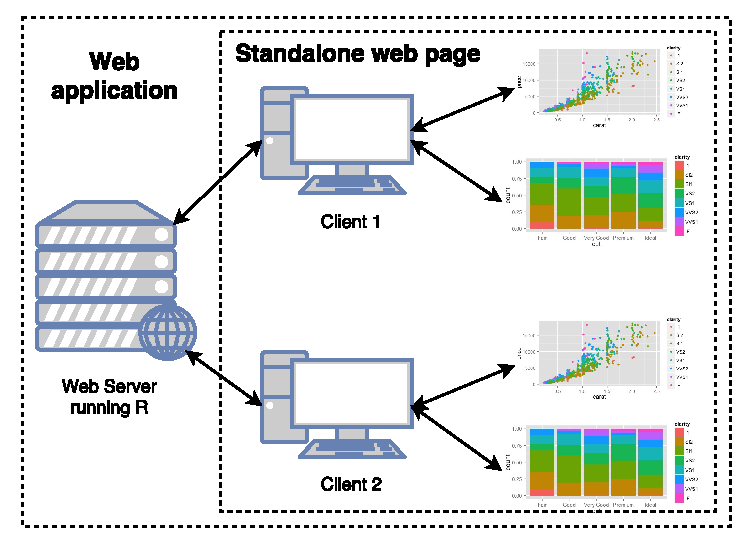
\includegraphics{images/server-client.pdf}
\caption{\label{fig:server-client}A basic visual depiction of the different
approaches to implementing a data pipeline for interactive web graphics.
The R packages \textbf{ggvis} and \textbf{shiny} expose the pipeline to
users in R, which requires a web server for viewing. The R package
\textbf{crosstalk} will allow developers to implement and expose the
pipeline on both the server and client levels.}
\end{figure}

Generally speaking, websites that render entirely client-side are more
desirable since they are easier to share, more responsive, and require
less computational resources to run\footnote{The
  \url{http://www.shinyapps.io/} service helps to provide easy access to
  a \textbf{shiny} server (a web server running special shiny software),
  so that \textbf{shiny} apps can be shared via a URL, for example:
  \url{https://hadley.shinyapps.io/14-ggvis/linked-brushing.Rmd}}.
However, the client-server approach can be very useful for dynamically
performing statistical computations, a key characteristic of most
interactive statistical graphics systems. (Urbanek and Horner
\protect\hyperlink{ref-FastRWeb}{2015}) and (Jeroen Ooms
\protect\hyperlink{ref-opencpu}{2014}\protect\hyperlink{ref-opencpu}{b})
also allow us to execute R code on a web server, and retrieve output via
HTTP, but \textbf{shiny} is the most heavily used since apps can be
written entirely in R using a very powerful, yet approachable, reactive
programming framework for handling user events. There are also many
convenient shortcuts for creating attractive HTML input forms, making it
incredibly easy to go from R script to an web app powered by R that
dynamically updates when users alter input values. In other words,
\textbf{shiny} makes it quick and easy to write web-based GUIs with
support for indirect manipulation.

Historically, an advanced understanding of \textbf{shiny} and JavaScript
was required to implement direct manipulation in a \textbf{shiny} app.
Recently, \textbf{shiny} added support for retrieving information on
user events with static R graphics\footnote{This website shows what
  information is sent from the client to the server when users interact
  with plot(s) via mouse event(s) --
  \url{http://shiny.rstudio.com/gallery/plot-interaction-basic.html}},
allowing developers to coordinate views in a web app, with no JavaScript
involved. This is a powerful tool for R users, but it has its
weaknesses. Most importantly, its not clear how to handle interactions
when positional scales are categorical (e.g., a bar chart) or how to
provide a visual clue that something has been selected.

The touring video in Figure \ref{fig:touR} purposefully uses
\textbf{shiny}'s built-in support for brushing to demonstrate the
problem with providing a visual clue. This points to the fundamental
problem in using non-web-based graphics to implement interactive
graphics in a web browser: every time the view updates, the display must
be redrawn, resulting in a ``glitch'' effect. If the plot being brushed
used native web graphics (e.g., SVG), it would allow for finer control
over how the view updates in response to user interactions and/or
dynamic data. On the other hand, since \textbf{ggvis} is web-based, and
has special client-side functionality, it knows how to smoothly
transition from one frame to the next when provided with new data from
the \textbf{shiny} server, which is crucial for constructing a mental
model of the data space. Having richer interfaces for generating
web-based interactive graphics from R that can share selections, and
handle smooth transitions, would make this, and many other examples,
generally better.

Many web-based graphing toolkits have appeared since the advent of
\textbf{rCharts}, making a single package that interfaces with
\emph{every} toolkit infeasible. Some ideas deriving from work on
\textbf{rCharts}, such as providing the glue to render plots in various
contexts (e.g., the R console, shiny apps, and \textbf{rmarkdown}
documents), have evolved into the R package \textbf{htmlwidgets}
(Vaidyanathan et al. \protect\hyperlink{ref-htmlwidgets}{2015}). Having
built similar bridges for \textbf{animint} and \textbf{LDAvis}, I
personally know and appreciate the amount of time and effort this
package saves other package authors.

The \textbf{htmlwidgets} framework is not constrained to just graphics,
it simply provides a set of conventions for authoring web content from
R. Numerous JavaScript data visualization libraries are now made
available using this framework, most designed for particular use cases,
such as \textbf{leaflet} for geo-spatial mapping, \textbf{dygraphs} for
time-series, and \textbf{networkD3} for networks (Cheng and Xie
\protect\hyperlink{ref-leaflet}{2015}); (Vanderkam and Allaire
\protect\hyperlink{ref-dygraphs}{2015}); (Gandrud, Allaire, and Russell
\protect\hyperlink{ref-networkD3}{2015}).\footnote{For more examples and
  information, see \url{http://www.htmlwidgets.org/} and
  \url{http://hafen.github.io/htmlwidgetsgallery/}} There are also HTML
widgets that provide an interface to more general purpose visualization
JavaScript libraries such as \textbf{plotly}, \textbf{rbokeh}, and
\textbf{rcdimple} (Sievert et al. \protect\hyperlink{ref-plotly}{2016});
(Hafen and team \protect\hyperlink{ref-rbokeh}{2015}); (Kiernander et
al. \protect\hyperlink{ref-rcdimple}{2015}). Most of these JavaScript
libraries provide at least some native support for direct manipulation
such as identifying (i.e., mousing over points to reveal labels),
focusing (i.e., pan and zoom), and sometimes highlighting (i.e.,
brushing over points to highlight points in another view). More often
than not, the support for dynamic and linked views is lacking,
especially if we want to define the linking in R, and produce a
standalone HTML document.

The R package \textbf{crosstalk} is a new framework for coordinating
arbitrary HTML widgets (Cheng
\protect\hyperlink{ref-crosstalk}{2015}\protect\hyperlink{ref-crosstalk}{a}).
It provides both an R and a JavaScript API for querying selections,
meaning \textbf{crosstalk} powered HTML widgets can work with or without
\textbf{shiny}, and if implemented carefully by HTML widget authors,
provides a means for coordinating multiple HTML widgets without shiny.
Generally speaking, \textbf{crosstalk} just provides a standard way to
set, store, and access selection values in the browser, so the actual
logic for updating views based on the selection value(s) is on the HTML
widget author, and this part is far from trivial. In a sense, this
project is similar to the work of North and Shneiderman
(\protect\hyperlink{ref-North:1999vi}{1999}), which provides semantics
for ``snapping together'' arbitrary views that are aware of the
relational schema, but does so in a web-based environment, rather than
requiring a machine running Windows.

The first HTML widget to leverage \textbf{crosstalk} was (Cheng
\protect\hyperlink{ref-d3scatter}{2015}\protect\hyperlink{ref-d3scatter}{b}),
but is limited to linked brushing on scatterplots.\footnote{See, for
  example, \url{http://rpubs.com/jcheng/crosstalk-demo}} Currently,
there are a couple other R packages with \textbf{crosstalk} support,
including \textbf{leaflet} and \textbf{listviewer}, but \textbf{plotly}
is the only package which supports a non-identity functions between the
data and displays. It also has rich support for interaction types,
including mouse hover, click, and multiple types of click+drag
selections.

Having HTML widgets that can share selections with each other will be a
huge step forward for web-based interactive graphics. With some effort
and careful implementation by HTML widget authors, it may be possible to
provide sensible defaults for updating views between arbitrary widgets,
and users that know some JavaScript will also be able to customize or
extend these defaults from R. The \textbf{htmlwidget} package provides
conventions for this, by allowing one to send arbitrary JavaScript
functions from R that execute after the widget has rendered in the
browser. The biggest problem in implementing coordinated widgets will be
in managing data structures, since each widget will likely have its own
data structure for representing a selection. In this case, in order to
coordinate them, users may have to embed widgets in a shiny app to
access and organize selections. This gives users tremendous control over
sharing selections, but may limit control over smooth transitions
between states of a given widget (a key characteristic of dynamic
graphics), and increases the amount of complexity involved in sharing
their work.

\chapter{Taming PITCHf/x Data with XML2R and pitchRx}

This chapter is a paper published in \emph{The R Journal} (Sievert
\protect\hyperlink{ref-Sievert:2014a}{2014}\protect\hyperlink{ref-Sievert:2014a}{b}).
I am the sole author of the paper which is avaliable online here
\url{https://journal.r-project.org/archive/2014-1/sievert.pdf}

The formatting of paper has been modified to make for consistent
typesetting across the thesis.

\specialchapt{ABSTRACT}

\textbf{XML2R} is a framework that reduces the effort required to
transform XML content into tables in a way that preserves parent to
child relationships. \textbf{pitchRx} applies \textbf{XML2R}'s grammar
for XML manipulation to Major League Baseball Advanced Media (MLBAM)'s
Gameday data. With \textbf{pitchRx}, one can easily obtain and store
Gameday data in a remote database. The Gameday website hosts a wealth of
XML data, but perhaps most interesting is PITCHf/x. Among other things,
PITCHf/x data can be used to recreate a baseball's flight path from a
pitcher's hand to home plate. With \textbf{pitchRx}, one can easily
create animations and interactive 3D scatterplots of the baseball's
flight path. PITCHf/x data is also commonly used to generate a static
plot of baseball locations at the moment they cross home plate. These
plots, sometimes called \textit{strike-zone plots}, can also refer to a
plot of event probabilities over the same region. \textbf{pitchRx}
provides an easy and robust way to generate strike-zone plots using the
\textbf{ggplot2} package.

\section{Introduction}\label{introduction}

\subsection{What is PITCHf/x?}\label{what-is-pitchfx}

PITCHf/x is a general term for a system that generates a series of 3D
measurements of a baseball's path from a pitcher's hand to home plate
(Alt and White \protect\hyperlink{ref-patent}{2008}).
\footnote{A \textit{pitcher} throws a ball to the opposing \textit{batter}, who
stands besides home plate and tries to hit the ball into the field
of play.
} In an attempt to estimate the location of the ball at any time point,
a quadratic regression model with nine parameters (defined by the
equations of motion for constant linear acceleration) is fit to each
pitch. Studies with access to the actual measurements suggest that this
model is quite reasonable -- especially for non-knuckleball pitches
(Nathan \protect\hyperlink{ref-trajecoryAnalysis}{2008}). That is, the
fitted path often provides a reasonable estimate (within a couple of
inches) of the actual locations. Unfortunately, only the parameter
estimates are made available to the public. The website that provides
these estimates is maintained by MLBAM and hosts a wealth of other
baseball related data used to inform MLB's Gameday webcast service in
near real time.

\subsection{Why is PITCHf/x important?}\label{why-is-pitchfx-important}

On the business side of baseball, using statistical analysis to scout
and evaluate players has become mainstream. When PITCHf/x was first
introduced, DiMeo (\protect\hyperlink{ref-slate}{2007}) proclaimed it
as,

\begin{quote} ``The new technology that will change statistical analysis [of baseball] forever.'' \end{quote}

PITCHf/x has yet to fully deliver this claim, partially due to the
difficulty in accessing and deriving insight from the large amount of
complex information. By providing better tools to collect and visualize
this data, \textbf{pitchRx} makes PITCHf/x analysis more accessible to
the general public.

\subsection{PITCHf/x applications}\label{pitchfx-applications}

PITCHf/x data is and can be used for many different projects. It can
also complement other baseball data sources, which poses an interesting
database management problem. Statistical analysis of PITCHf/x data and
baseball in general has become so popular that it has helped expose
statistical ideas and practice to the general public. If you have
witnessed television broadcasts of MLB games, you know one obvious
application of PITCHf/x is locating pitches in the strike-zone as well
as recreating flight trajectories, tracking pitch speed, etc. Some
on-going statistical research related to PITCHf/x includes: classifying
pitch types, predicting pitch sequences, and clustering pitchers with
similar tendencies (Pane et al. \protect\hyperlink{ref-curve}{2013}).

\subsection[Contributions of pitchRx and XML2R]{Contributions of \textbf{pitchRx} and \textbf{XML2R}}

The \textbf{pitchRx} package has two main focuses (Sievert
\protect\hyperlink{ref-pitchRx}{2014}\protect\hyperlink{ref-pitchRx}{a}).
The first focus is to provide easy access to Gameday data. Not only is
\textbf{pitchRx} helpful for collecting this data in bulk, but it has
served as a helpful teaching and research aide
(\url{http://baseballwithr.wordpress.com/} is one such example). Methods
for collecting Gameday data existed prior to \textbf{pitchRx}; however,
these methods are not easily extensible and require juggling
technologies that may not be familiar or accessible (Fast
\protect\hyperlink{ref-database}{2007}). Moreover, these working
environments are less desirable than R for data analysis and
visualization. Since \textbf{pitchRx} is built upon \textbf{XML2R}'s
united framework, it can be easily modified and/or extended (Sievert
\protect\hyperlink{ref-XML2R}{2014}\protect\hyperlink{ref-XML2R}{c}).
For this same reason, \textbf{pitchRx} serves as a model for building
customized XML data collection tools with \textbf{XML2R}.

The other main focus of \textbf{pitchRx} is to simplify the process
creating popular PITCHf/x graphics. Strike-zone plots and animations
made via \textbf{pitchRx} utilize the extensible \textbf{ggplot2}
framework as well as various customized options (Wickham
\protect\hyperlink{ref-ggplot2}{2009}\protect\hyperlink{ref-ggplot2}{a}).
\textbf{ggplot2} is a convenient framework for generating strike-zone
plots primarily because of its facet schema which allows one to make
visual comparisons across any combination of discrete variable(s).
Interactive 3D scatterplots are based on the \textbf{rgl} package and
useful for gaining a new perspective on flight trajectories (Adler,
Murdoch, and others \protect\hyperlink{ref-rgl}{2016}).

\section{Getting familiar with
Gameday}\label{getting-familiar-with-gameday}

Gameday data is hosted and made available for free thanks to MLBAM via
\url{http://gd2.mlb.com/components/game/mlb/}.
\footnote{Please be respectful of this service and store any information after
you extract it instead of repeatedly querying the website. Before
using any content from this website, please also read the \href{http://gdx.mlb.com/components/copyright.txt}{copyright}.
} From this website, one can obtain many different types of data besides
PITCHf/x. For example, one can obtain everything from
\href{http://gd2.mlb.com/components/game/mlb/year_2013/month_07/day_16/gid_2013_07_16_aasmlb_nasmlb_1/media/instadium.xml}{structured media metadata}
to
\href{http://gd2.mlb.com/components/game/mlb/twitter/anaInsiderTweets.xml}{insider tweets}.
In fact, this website's purpose is to serve data to various
\url{http://mlb.com} web pages and applications. As a result, some data
is redundant and the format may not be optimal for statistical analysis.
For these reasons, the \texttt{scrape} function is focused on retrieving
data that is useful for PITCHf/x analysis and providing it in a
convenient format for data analysis.

Navigating through the MLBAM website can be overwhelming, but it helps
to recognize that a homepage exists for nearly every day and every game.
For example,
\url{http://gd2.mlb.com/components/game/mlb/year_2011/month_02/day_26/}
displays numerous hyperlinks to various files specific to February 26th,
2011. On this page is a hyperlink to
\href{http://gd2.mlb.com/components/game/mlb/year_2011/month_02/day_26/miniscoreboard.xml}{miniscoreboard.xml}
which contains information on every game played on that date. This page
also has numerous hyperlinks to game specific pages. For example,
\href{http://gd2.mlb.com/components/game/mlb/year_2011/month_02/day_26/gid_2011_02_26_phimlb_nyamlb_1/}{gid\_2011\_02\_26\_phimlb\_nyamlb\_1/}
points to the homepage for that day's game between the NY Yankees and
Philadelphia Phillies. On this page is a hyperlink to the
\href{http://gd2.mlb.com/components/game/mlb/year_2011/month_02/day_26/gid_2011_02_26_phimlb_nyamlb_1/players.xml}{players.xml}
file which contains information about the players, umpires, and coaches
(positions, names, batting average, etc.) coming into that game.

Starting from a particular game's homepage and clicking on the
\href{http://gd2.mlb.com/components/game/mlb/year_2011/month_02/day_26/gid_2011_02_26_phimlb_nyamlb_1/inning/}{inning/}
directory, we \emph{should} see another page with links to the
\href{http://gd2.mlb.com/components/game/mlb/year_2011/month_02/day_26/gid_2011_02_26_phimlb_nyamlb_1/inning/inning_all.xml}{inning\_all.xml}
file and the
\href{http://gd2.mlb.com/components/game/mlb/year_2011/month_02/day_26/gid_2011_02_26_phimlb_nyamlb_1/inning/inning_hit.xml}{inning\_hit.xml}
file. If it is available, the \texttt{inning\_all.xml} file contains the
PITCHf/x data for that game. It's important to note that this file won't
exist for some games, because some games are played in venues that do
not have a working PITCHf/x system in place. This is especially true for
preseason games and games played prior to the 2008 season when the
PITCHf/x system became widely adopted.
\footnote{In this case, \texttt{scrape} will print ``failed to load HTTP resource''
in the R console (after the relevant file name) to indicate that no
data was available.
} The \texttt{inning\_hit.xml} files have manually recorded spatial
coordinates of where a home run landed or where the baseball made
initial contact with a defender after it was hit into play.

The relationship between these XML files and the tables returned by
\texttt{scrape} is presented in Table \ref{table:pitchfx}. The
\texttt{pitch} table is extracted from files whose name ends in
\texttt{inning\_all.xml}. This is the only table returned by
\texttt{scrape} that contains data on the pitch-by-pitch level. The
\texttt{atbat}, \texttt{runner}, \texttt{action} and \texttt{hip} tables
from this same file are commonly labeled somewhat ambiguously as
play-by-play data. The \texttt{player}, \texttt{coach}, and
\texttt{umpire} tables are extracted from \texttt{players.xml} and are
classified as game-by-game since there is one record per person per
game. Figure \ref{fig:relations} shows how these tables can be connected
to one another in a database setting. The direction of the arrows
represent a one to possibly many relationship. For example, at least one
pitch is thrown for each \textit{at bat} (that is, each bout between
pitcher and batter) and there are numerous at bats within each game.

In a rough sense, one can relate tables returned by \texttt{scrape} back
to XML nodes in the XML files. For convenience, some information in
certain XML nodes are combined into one table. For example, information
gleaned from the `top', `bottom', and `inning' XML nodes within
\texttt{inning\_all.xml} are included as \texttt{inning} and
\texttt{inning\_side} fields in the \texttt{pitch}, \texttt{po},
\texttt{atbat}, \texttt{runner}, and \texttt{action} tables. This helps
reduce the burden of merging many tables together in order to have
inning information on the play-by-play and/or pitch-by-pitch level.
Other information is simply ignored simply because it is redundant. For
example, the `game' node within the \texttt{players.xml} file contains
information that can be recovered from the \texttt{game} table extracted
from the \texttt{miniscoreboard.xml} file. If the reader wants a more
detailed explanation of fields in these tables, Marchi and Albert
(\protect\hyperlink{ref-baseball}{2013}) provide nice overview.

\begin{table}

\caption{\label{tab:pitchfx}Structure of PITCHf/x and related Gameday data sources accessible to `scrape()`}
\centering
\begin{tabular}[t]{llll}
\toprule
Source file & Information & XML nodes & Tables Returned\\
\midrule
miniscoreboard.xml & game-by-game & games, game & game, media\\
 &  & game\_media, media & \\
players.xml & game-by-game & game, team, player, & player, coach,\\
 &  & coach, umpire & umpire\\
inning\_all.xml & play-by-play, & game, inning, bottom, & atbat, po,\\
\addlinespace
 & pitch-by-pitch & top, atbat, po, & pitch, runner,\\
 &  & pitch, runner action & action\\
inning\_hit.xml & play-by-play & hitchart, hip & hip\\
\bottomrule
\end{tabular}
\end{table}

\begin{figure}[htbp]
\centering
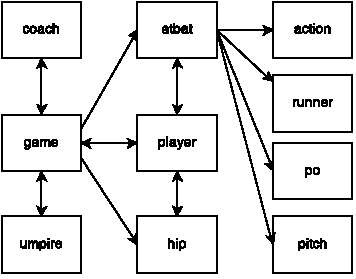
\includegraphics{images/Drawing1.pdf}
\caption{\label{fig:relations}Table relations between Gameday data
accessible via \texttt{scrape()}. The direction of the arrows indicate a
one to possibly many relationship.}
\end{figure}

\section{Introducing XML2R}\label{introducing-xml2r}

\textbf{XML2R} adds to the
\href{http://cran.r-project.org/web/views/WebTechnologies.html}{CRAN Task View on Web Technologies and Services}
by focusing on the transformation of XML content into a collection of
tables. Compared to a lower-level API like the \textbf{XML} package, it
can significantly reduce the amount of coding and cognitive effort
required to perform such a task. In contrast to most higher-level APIs,
it does not make assumptions about the XML structure or its source.
Although \textbf{XML2R} works on any structure, performance and user
experience are enhanced if the content has an inherent relational
structure. \textbf{XML2R}'s novel approach to XML data collection breaks
down the transformation process into a few simple steps and allows the
user to decide how to apply those steps.

The next few sections demonstrate how \textbf{pitchRx} leverages
\textbf{XML2R} in order to produce a collection of tables from
\texttt{inning\_all.xml} files. A similar approach is used by
\texttt{pitchRx::scrape} to construct tables from the other Gameday
files in Table \ref{table:pitchfx}. In fact, \textbf{XML2R} has also
been used in the R package
\href{https://github.com/cpsievert/bbscrapeR}{bbscrapeR} which collects
data from \href{http://nba.com}{nba.com} and
\href{http://wnba.com}{wnba.com}.

\subsection{Constructing file names}\label{constructing-file-names}

Sometimes the most frustrating part of obtaining data in bulk off of the
web is finding the proper collection of URLs or file names of interest.
Since files on the Gameday website are fairly well organized, the
\texttt{makeUrls} function can be used to construct \texttt{urls} that
point to every game's homepage within a window of dates.

\begin{Shaded}
\begin{Highlighting}[]
\NormalTok{urls <-}\StringTok{ }\NormalTok{pitchRx::}\KeywordTok{makeUrls}\NormalTok{(}\DataTypeTok{start =} \StringTok{"2011-06-01"}\NormalTok{, }\DataTypeTok{end =} \StringTok{"2011-06-01"}\NormalTok{) }
\KeywordTok{sub}\NormalTok{(}\StringTok{"http://gd2.mlb.com/components/game/mlb/"}\NormalTok{, }\StringTok{""}\NormalTok{, }\KeywordTok{head}\NormalTok{(urls))}
\CommentTok{#> [1] "year_2011/month_06/day_01/gid_2011_06_01_anamlb_kcamlb_1"}
\CommentTok{#> [2] "year_2011/month_06/day_01/gid_2011_06_01_balmlb_seamlb_1"}
\CommentTok{#> [3] "year_2011/month_06/day_01/gid_2011_06_01_chamlb_bosmlb_1"}
\CommentTok{#> [4] "year_2011/month_06/day_01/gid_2011_06_01_clemlb_tormlb_1"}
\CommentTok{#> [5] "year_2011/month_06/day_01/gid_2011_06_01_colmlb_lanmlb_1"}
\CommentTok{#> [6] "year_2011/month_06/day_01/gid_2011_06_01_flomlb_arimlb_1"}
\end{Highlighting}
\end{Shaded}

\subsection{Extracting observations}\label{extracting-observations}

Once we have a collection of XML \texttt{files}, the next step is to
parse the content into a list of \textit{observations}. An observation
is technically defined as a matrix with one row and some number of
columns. The columns are defined by XML attributes and the XML value (if
any) for a particular XML lineage. The name of each observation tracks
the XML hierarchy so observations can be grouped together in a sensible
fashion at a later point.

\begin{Shaded}
\begin{Highlighting}[]
\KeywordTok{library}\NormalTok{(XML2R)}
\NormalTok{files <-}\StringTok{ }\KeywordTok{paste0}\NormalTok{(urls, }\StringTok{"/inning/inning_all.xml"}\NormalTok{)}
\NormalTok{obs <-}\StringTok{ }\KeywordTok{XML2Obs}\NormalTok{(files, }\DataTypeTok{url.map =} \OtherTok{TRUE}\NormalTok{, }\DataTypeTok{quiet =} \OtherTok{TRUE}\NormalTok{) }
\KeywordTok{table}\NormalTok{(}\KeywordTok{names}\NormalTok{(obs))}
\CommentTok{#> }
\CommentTok{#>                                game                        game//inning }
\CommentTok{#>                                  15                                 137 }
\CommentTok{#>        game//inning//bottom//action         game//inning//bottom//atbat }
\CommentTok{#>                                 116                                 532 }
\CommentTok{#>  game//inning//bottom//atbat//pitch     game//inning//bottom//atbat//po }
\CommentTok{#>                                1978                                  61 }
\CommentTok{#> game//inning//bottom//atbat//runner           game//inning//top//action }
\CommentTok{#>                                 373                                 150 }
\CommentTok{#>            game//inning//top//atbat     game//inning//top//atbat//pitch }
\CommentTok{#>                                 593                                2183 }
\CommentTok{#>        game//inning//top//atbat//po    game//inning//top//atbat//runner }
\CommentTok{#>                                  75                                 509 }
\CommentTok{#>                             url_map }
\CommentTok{#>                                   1}
\end{Highlighting}
\end{Shaded}

This output tells us that 247 pitches were thrown in the bottom inning
and 278 were thrown in the top inning on June 1st, 2011. Also, there are
12 different levels of observations. The list element named
\texttt{url\_map} is not considered an observation and was included
since \texttt{url.map = TRUE}. This helps avoid repeating long file
names in the \texttt{url\_key} column which tracks the mapping between
observations and file names.

\begin{Shaded}
\begin{Highlighting}[]
\NormalTok{obs[}\DecValTok{1}\NormalTok{]}
\CommentTok{#> $`game//inning//top//atbat//pitch`}
\CommentTok{#>      des             des_es           id  type tfs     }
\CommentTok{#> [1,] "Called Strike" "Strike cantado" "3" "S"  "201107"}
\CommentTok{#>      tfs_zulu               x        y        event_num sv_id          }
\CommentTok{#> [1,] "2011-06-01T20:11:07Z" "103.00" "149.38" "3"       "110601_151108"}
\CommentTok{#>      play_guid start_speed end_speed sz_top sz_bot pfx_x   pfx_z  px      }
\CommentTok{#> [1,] ""        "94.0"      "86.1"    "2.85" "1.36" "-8.12" "11.0" "-0.143"}
\CommentTok{#>      pz      x0       y0     z0      vx0     vy0        vz0      ax       }
\CommentTok{#> [1,] "2.376" "-2.435" "50.0" "5.831" "9.058" "-137.334" "-7.288" "-15.446"}
\CommentTok{#>      ay       az        break_y break_angle break_length pitch_type}
\CommentTok{#> [1,] "31.474" "-11.175" "23.8"  "46.3"      "4.0"        "FF"      }
\CommentTok{#>      type_confidence zone nasty spin_dir  spin_rate  cc mt url_key}
\CommentTok{#> [1,] ".865"          "2"  "46"  "216.336" "2753.789" "" "" "url1"}
\end{Highlighting}
\end{Shaded}

\subsection{Renaming observations}\label{renaming-observations}

Before grouping observations into a collection tables based on their
names, one may want to \texttt{re\_name} observations. Observations with
names \texttt{'game//inning//bottom//atbat'} and
\texttt{'game//inning//top//atbat'} should be included in the same table
since they share XML attributes (in other words, the observations share
variables).

\begin{Shaded}
\begin{Highlighting}[]
\NormalTok{tmp <-}\StringTok{ }\KeywordTok{re_name}\NormalTok{(obs, }\DataTypeTok{equiv =} \KeywordTok{c}\NormalTok{(}\StringTok{"game//inning//top//atbat"}\NormalTok{,                             }
  \StringTok{"game//inning//bottom//atbat"}\NormalTok{), }\DataTypeTok{diff.name =} \StringTok{"inning_side"}\NormalTok{) }
\end{Highlighting}
\end{Shaded}

By passing these names to the \texttt{equiv} argument, \texttt{re\_name}
determines the difference in the naming scheme and suppresses that
difference. In other words, observation names that match the
\texttt{equiv} argument will be renamed to
\texttt{'game//inning//atbat'}. The information removed from the name is
not lost; however, as a new column is appended to the end of each
relevant observation. For example, notice how the \texttt{inning\_side}
column contains the part of the name we just removed:

\begin{Shaded}
\begin{Highlighting}[]
\NormalTok{tmp[}\KeywordTok{grep}\NormalTok{(}\StringTok{"game//inning//atbat"}\NormalTok{, }\KeywordTok{names}\NormalTok{(tmp))][}\DecValTok{1}\NormalTok{:}\DecValTok{2}\NormalTok{]}
\CommentTok{#> $`game//inning//atbat`}
\CommentTok{#>      num b   s   o   start_tfs start_tfs_zulu         batter   stand}
\CommentTok{#> [1,] "1" "3" "2" "0" "201034"  "2011-06-01T20:10:34Z" "430947" "L"  }
\CommentTok{#>      b_height pitcher  p_throws}
\CommentTok{#> [1,] "5-10"   "462956" "R"     }
\CommentTok{#>      des                                                                     }
\CommentTok{#> [1,] "Erick Aybar singles on a line drive to center fielder Melky Cabrera.  "}
\CommentTok{#>      des_es                                                                    }
\CommentTok{#> [1,] "Erick Aybar pega sencillo con línea a jardinero central Melky Cabrera.  "}
\CommentTok{#>      event_num event    event_es   home_team_runs away_team_runs url_key}
\CommentTok{#> [1,] "12"      "Single" "Sencillo" "0"            "0"            "url1" }
\CommentTok{#>      inning_side}
\CommentTok{#> [1,] "top"      }
\CommentTok{#> }
\CommentTok{#> $`game//inning//atbat`}
\CommentTok{#>      num b   s   o   start_tfs start_tfs_zulu         batter   stand}
\CommentTok{#> [1,] "2" "2" "3" "1" "201412"  "2011-06-01T20:14:12Z" "110029" "L"  }
\CommentTok{#>      b_height pitcher  p_throws des                                   }
\CommentTok{#> [1,] "6-0"    "462956" "R"      "Bobby Abreu called out on strikes.  "}
\CommentTok{#>      des_es                                 event_num event       event_es}
\CommentTok{#> [1,] "Bobby Abreu se poncha sin tirarle.  " "24"      "Strikeout" "Ponche"}
\CommentTok{#>      home_team_runs away_team_runs url_key inning_side}
\CommentTok{#> [1,] "0"            "0"            "url1"  "top"}
\end{Highlighting}
\end{Shaded}

For similar reasons, other observation name pairs are renamed in a
similar fashion.

\begin{Shaded}
\begin{Highlighting}[]
\NormalTok{tmp <-}\StringTok{ }\KeywordTok{re_name}\NormalTok{(tmp, }\DataTypeTok{equiv =} \KeywordTok{c}\NormalTok{(}\StringTok{"game//inning//top//atbat//runner"}\NormalTok{,                             }
  \StringTok{"game//inning//bottom//atbat//runner"}\NormalTok{), }\DataTypeTok{diff.name =} \StringTok{"inning_side"}\NormalTok{)}
\NormalTok{tmp <-}\StringTok{ }\KeywordTok{re_name}\NormalTok{(tmp, }\DataTypeTok{equiv =} \KeywordTok{c}\NormalTok{(}\StringTok{"game//inning//top//action"}\NormalTok{,                             }
  \StringTok{"game//inning//bottom//action"}\NormalTok{), }\DataTypeTok{diff.name =} \StringTok{"inning_side"}\NormalTok{)  }
\NormalTok{tmp <-}\StringTok{ }\KeywordTok{re_name}\NormalTok{(tmp, }\DataTypeTok{equiv =} \KeywordTok{c}\NormalTok{(}\StringTok{"game//inning//top//atbat//po"}\NormalTok{,                            }
  \StringTok{"game//inning//bottom//atbat//po"}\NormalTok{), }\DataTypeTok{diff.name =} \StringTok{"inning_side"}\NormalTok{)}
\NormalTok{obs2 <-}\StringTok{ }\KeywordTok{re_name}\NormalTok{(tmp, }\DataTypeTok{equiv =} \KeywordTok{c}\NormalTok{(}\StringTok{"game//inning//top//atbat//pitch"}\NormalTok{,                             }
  \StringTok{"game//inning//bottom//atbat//pitch"}\NormalTok{), }\DataTypeTok{diff.name =} \StringTok{"inning_side"}\NormalTok{) }
\KeywordTok{table}\NormalTok{(}\KeywordTok{names}\NormalTok{(obs2))}
\CommentTok{#> }
\CommentTok{#>                        game                game//inning }
\CommentTok{#>                          15                         137 }
\CommentTok{#>        game//inning//action         game//inning//atbat }
\CommentTok{#>                         266                        1125 }
\CommentTok{#>  game//inning//atbat//pitch     game//inning//atbat//po }
\CommentTok{#>                        4161                         136 }
\CommentTok{#> game//inning//atbat//runner                     url_map }
\CommentTok{#>                         882                           1}
\end{Highlighting}
\end{Shaded}

\subsection{Linking observations}\label{linking-observations}

After all that renaming, we now have 7 different levels of observations.
Let's examine the first three observations on the \texttt{game//inning}
level:

\begin{Shaded}
\begin{Highlighting}[]
\NormalTok{obs2[}\KeywordTok{grep}\NormalTok{(}\StringTok{"^game//inning$"}\NormalTok{, }\KeywordTok{names}\NormalTok{(obs2))][}\DecValTok{1}\NormalTok{:}\DecValTok{3}\NormalTok{] }
\CommentTok{#> $`game//inning`}
\CommentTok{#>      num away_team home_team next url_key}
\CommentTok{#> [1,] "1" "ana"     "kca"     "Y"  "url1" }
\CommentTok{#> }
\CommentTok{#> $`game//inning`}
\CommentTok{#>      num away_team home_team next url_key}
\CommentTok{#> [1,] "2" "ana"     "kca"     "Y"  "url1" }
\CommentTok{#> }
\CommentTok{#> $`game//inning`}
\CommentTok{#>      num away_team home_team next url_key}
\CommentTok{#> [1,] "3" "ana"     "kca"     "Y"  "url1"}
\end{Highlighting}
\end{Shaded}

Before grouping observations into tables, it is usually important
preserve the parent-to-child relationships in the XML lineage. For
example, one may want to map a particular pitch back to the inning in
which it was thrown. Using the \texttt{add\_key} function, the relevant
value of \texttt{num} for \texttt{game//inning} observations can be
\texttt{recycle}d to its XML descendants.

\begin{Shaded}
\begin{Highlighting}[]
\NormalTok{obswkey <-}\StringTok{ }\KeywordTok{add_key}\NormalTok{(obs2, }\DataTypeTok{parent =} \StringTok{"game//inning"}\NormalTok{, }\DataTypeTok{recycle =} \StringTok{"num"}\NormalTok{, }\DataTypeTok{key.name =} \StringTok{"inning"}\NormalTok{)}
\end{Highlighting}
\end{Shaded}

As it turns out, the \texttt{away\_team} and \texttt{home\_team} columns
are redundant as this information is embedded in the \texttt{url}
column. Thus, there is only one other informative attribute on this
level which is \texttt{next}. By recycling this value among its
descendants, we remove any need to retain a \texttt{game//inning} table.

\begin{Shaded}
\begin{Highlighting}[]
\NormalTok{obswkey <-}\StringTok{ }\KeywordTok{add_key}\NormalTok{(obswkey, }\DataTypeTok{parent =} \StringTok{"game//inning"}\NormalTok{, }\DataTypeTok{recycle =} \StringTok{"next"}\NormalTok{)}
\end{Highlighting}
\end{Shaded}

It is also imperative that we can link a \texttt{pitch},
\texttt{runner}, or \texttt{po} back to a particular \texttt{atbat}.
This can be done as follows:

\begin{Shaded}
\begin{Highlighting}[]
\NormalTok{obswkey <-}\StringTok{ }\KeywordTok{add_key}\NormalTok{(obswkey, }\DataTypeTok{parent =} \StringTok{"game//inning//atbat"}\NormalTok{, }\DataTypeTok{recycle =} \StringTok{"num"}\NormalTok{)}
\end{Highlighting}
\end{Shaded}

\subsection{Collapsing observations}\label{collapsing-observations}

Finally, we are in a position to pool together observations that have a
common name. The \texttt{collapse\_obs} function achieves this by row
binding observations with the same name together and returning a list of
matrices. Note that \texttt{collapse\_obs} does not require that
observations from the same level to have the same set of variables in
order to be bound into a common table. In the case where variables are
missing, \texttt{NA}s will be inserted as values.

\begin{Shaded}
\begin{Highlighting}[]
\NormalTok{tables <-}\StringTok{ }\KeywordTok{collapse_obs}\NormalTok{(obswkey) }
\CommentTok{#As mentioned before, we do not need the 'inning' table }
\NormalTok{tables <-}\StringTok{ }\NormalTok{tables[!}\KeywordTok{grepl}\NormalTok{(}\StringTok{"^game//inning$"}\NormalTok{, }\KeywordTok{names}\NormalTok{(tables))]      }
\NormalTok{table.names <-}\StringTok{ }\KeywordTok{c}\NormalTok{(}\StringTok{"game"}\NormalTok{, }\StringTok{"action"}\NormalTok{, }\StringTok{"atbat"}\NormalTok{, }\StringTok{"pitch"}\NormalTok{, }\StringTok{"po"}\NormalTok{, }\StringTok{"runner"}\NormalTok{) }
\NormalTok{tables <-}\StringTok{ }\KeywordTok{setNames}\NormalTok{(tables, table.names) }
\KeywordTok{head}\NormalTok{(tables[[}\StringTok{"runner"}\NormalTok{]])}
\CommentTok{#>      id       start end  event                event_num url_key}
\CommentTok{#> [1,] "430947" ""    "1B" "Single"             "12"      "url1" }
\CommentTok{#> [2,] "430947" "1B"  "2B" "Stolen Base 2B"     "19"      "url1" }
\CommentTok{#> [3,] "430947" "2B"  "3B" "Groundout"          "30"      "url1" }
\CommentTok{#> [4,] "430947" "3B"  ""   "Groundout"          "36"      "url1" }
\CommentTok{#> [5,] "543333" ""    "1B" "Single"             "58"      "url1" }
\CommentTok{#> [6,] "543333" "1B"  ""   "Pickoff Attempt 1B" "69"      "url1" }
\CommentTok{#>      inning_side inning next num score rbi earned}
\CommentTok{#> [1,] "top"       "1"    "Y"  "1" NA    NA  NA    }
\CommentTok{#> [2,] "top"       "1"    "Y"  "2" NA    NA  NA    }
\CommentTok{#> [3,] "top"       "1"    "Y"  "3" NA    NA  NA    }
\CommentTok{#> [4,] "top"       "1"    "Y"  "4" NA    NA  NA    }
\CommentTok{#> [5,] "bottom"    "1"    "Y"  "7" NA    NA  NA    }
\CommentTok{#> [6,] "bottom"    "1"    "Y"  "8" NA    NA  NA}
\end{Highlighting}
\end{Shaded}

\section{Collecting Gameday data with
pitchRx}\label{collecting-gameday-data-with-pitchrx}

The main scraping function in \textbf{pitchRx}, \texttt{scrape}, can be
used to easily obtain data from the files listed in Table
\ref{table:pitchfx}. In fact, any combination of these files can be
queried using the \texttt{suffix} argument. In the example below, the
\texttt{start} and \texttt{end} arguments are also used so that all
available file types for June 1st, 2011 are queried.

\begin{Shaded}
\begin{Highlighting}[]
\KeywordTok{library}\NormalTok{(pitchRx)}
\NormalTok{files <-}\StringTok{ }\KeywordTok{c}\NormalTok{(}\StringTok{"inning/inning_all.xml"}\NormalTok{, }\StringTok{"inning/inning_hit.xml"}\NormalTok{, }
  \StringTok{"miniscoreboard.xml"}\NormalTok{, }\StringTok{"players.xml"}\NormalTok{)}
\NormalTok{dat <-}\StringTok{ }\KeywordTok{scrape}\NormalTok{(}\DataTypeTok{start =} \StringTok{"2011-06-01"}\NormalTok{, }\DataTypeTok{end =} \StringTok{"2011-06-01"}\NormalTok{, }\DataTypeTok{suffix =} \NormalTok{files)}
\end{Highlighting}
\end{Shaded}

The \texttt{game.ids} option can be used instead of \texttt{start} and
\texttt{end} to obtain an equivalent \texttt{dat} object. This option
can be useful if the user wants to query specific games rather than all
games played over a particular time span. When using this
\texttt{game.ids} option, the built-in \texttt{gids} object, is quite
convenient.

\begin{Shaded}
\begin{Highlighting}[]
\KeywordTok{data}\NormalTok{(gids, }\DataTypeTok{package =} \StringTok{"pitchRx"}\NormalTok{)}
\NormalTok{gids11 <-}\StringTok{ }\NormalTok{gids[}\KeywordTok{grep}\NormalTok{(}\StringTok{"2011_06_01"}\NormalTok{, gids)]}
\KeywordTok{head}\NormalTok{(gids11)}
\CommentTok{#> [1] "gid_2011_06_01_anamlb_kcamlb_1" "gid_2011_06_01_balmlb_seamlb_1"}
\CommentTok{#> [3] "gid_2011_06_01_chamlb_bosmlb_1" "gid_2011_06_01_clemlb_tormlb_1"}
\CommentTok{#> [5] "gid_2011_06_01_colmlb_lanmlb_1" "gid_2011_06_01_flomlb_arimlb_1"}
\end{Highlighting}
\end{Shaded}

\begin{Shaded}
\begin{Highlighting}[]
\NormalTok{dat <-}\StringTok{ }\KeywordTok{scrape}\NormalTok{(}\DataTypeTok{game.ids =} \NormalTok{gids11, }\DataTypeTok{suffix =} \NormalTok{files)}
\end{Highlighting}
\end{Shaded}

The object \texttt{dat} is a list of data frames containing all data
available for June 1st, 2011 using \texttt{scrape}. The list names match
the table names provided in Table \ref{table:pitchfx}. For example,
\texttt{dat\$atbat} is data frame with every at bat on June 1st, 2011
and \texttt{dat\$pitch} has information related to the outcome of each
pitch (including PITCHf/x parameters). The \texttt{object.size} of
\texttt{dat} is nearly 300MB. Multiplying this number by 100 days
exceeds the memory of most machines. Thus, if a large amount of data is
required, the user should exploit the R database interface (R Special
Interest Group on Databases \protect\hyperlink{ref-DBI}{2013}).

\section{Storing and querying Gameday
data}\label{storing-and-querying-gameday-data}

Since PITCHf/x data can easily exhaust memory, one should consider
establishing a database instance before using \texttt{scrape}. By
passing a database connection to the \texttt{connect} argument,
\texttt{scrape} will try to create (and/or append to existing) tables
using that connection. If the connection fails for some reason, tables
will be written as csv files in the current working directory. The
benefits of using the \texttt{connect} argument includes improved memory
management which can greatly reduce run time. \texttt{connect} will
support a MySQL connection, but creating a SQLite database is quite easy
with \textbf{dplyr} (Wickham and Francois
\protect\hyperlink{ref-dplyr}{2014}).

\begin{Shaded}
\begin{Highlighting}[]
\KeywordTok{library}\NormalTok{(dplyr)}
\NormalTok{db <-}\StringTok{ }\KeywordTok{src_sqlite}\NormalTok{(}\StringTok{"GamedayDB.sqlite3"}\NormalTok{, }\DataTypeTok{create =} \OtherTok{TRUE}\NormalTok{)}
\CommentTok{# Collect and store all PITCHf/x data from 2008 to now}
\KeywordTok{scrape}\NormalTok{(}\DataTypeTok{start =} \StringTok{"2008-01-01"}\NormalTok{, }\DataTypeTok{end =} \KeywordTok{Sys.Date}\NormalTok{(), }
  \DataTypeTok{suffix =} \StringTok{"inning/inning_all.xml"}\NormalTok{, }\DataTypeTok{connect =} \NormalTok{db$con)}
\end{Highlighting}
\end{Shaded}

In the later sections, animations of four-seam and cut fastballs thrown
by Mariano Rivera and Phil Hughes during the 2011 season are created. In
order to obtain the data for those animations, one could query
\texttt{db} which now has PITCHf/x data from 2008 to date. This query
requires criteria on: the \texttt{pitcher\_name} field (in the
\texttt{atbat} table), the \texttt{pitch\_type} field (in the
\texttt{pitch} table), and the \texttt{date} field (in both tables). To
reduce the time required to search those records, one should create an
index on each of these three fields.

\begin{Shaded}
\begin{Highlighting}[]
\KeywordTok{library}\NormalTok{(DBI)}
\KeywordTok{dbSendQuery}\NormalTok{(db$con, }\StringTok{"CREATE INDEX pitcher_index ON atbat(pitcher_name)"}\NormalTok{) }
\KeywordTok{dbSendQuery}\NormalTok{(db$con, }\StringTok{"CREATE INDEX type_index ON pitch(pitch_type)"}\NormalTok{) }
\KeywordTok{dbSendQuery}\NormalTok{(db$con, }\StringTok{"CREATE INDEX date_atbat ON atbat(date)"}\NormalTok{) }
\end{Highlighting}
\end{Shaded}

As a part of our query, we'll have to join the \texttt{atbat} table
together with the \texttt{pitch} table. For this task, the
\texttt{gameday\_link} and \texttt{num} fields are helpful since
together they provide a way to match pitches with at bats. For this
reason, a multi-column index on the \texttt{gameday\_link} and
\texttt{num} fields will further reduce run time of the query.

\begin{Shaded}
\begin{Highlighting}[]
\KeywordTok{dbSendQuery}\NormalTok{(db$con, }\StringTok{'CREATE INDEX pitch_join ON pitch(gameday_link, num)'}\NormalTok{) }
\KeywordTok{dbSendQuery}\NormalTok{(db$con, }\StringTok{'CREATE INDEX atbat_join ON atbat(gameday_link, num)'}\NormalTok{)}
\end{Highlighting}
\end{Shaded}

Although the query itself could be expressed entirely in SQL,
\textbf{dplyr}'s grammar for data manipulation (which is database
agnostic) can help to simplify the task. In this case, \texttt{at.bat}
is a tabular \emph{representation} of the remote \texttt{atbat} table
restricted to cases where Rivera or Hughes was the pitcher. That is,
\texttt{at.bat} does not contain the actual data, but it does contain
the information necessary to retrieve it from the database.

\begin{Shaded}
\begin{Highlighting}[]
\NormalTok{at.bat <-}\StringTok{ }\KeywordTok{tbl}\NormalTok{(db, }\StringTok{"atbat"}\NormalTok{) %>%}\StringTok{   }
\StringTok{  }\KeywordTok{filter}\NormalTok{(pitcher_name %in%}\StringTok{ }\KeywordTok{c}\NormalTok{(}\StringTok{"Mariano Rivera"}\NormalTok{, }\StringTok{"Phil Hughes"}\NormalTok{))}
\end{Highlighting}
\end{Shaded}

Similarly, \texttt{fbs} is a tabular representation of the
\texttt{pitch} table restricted to four-seam (FF) and cut fastballs
(FC).

\begin{Shaded}
\begin{Highlighting}[]
\NormalTok{fbs <-}\StringTok{ }\KeywordTok{tbl}\NormalTok{(db, }\StringTok{"pitch"}\NormalTok{) %>%}\StringTok{      }
\StringTok{  }\KeywordTok{filter}\NormalTok{(pitch_type %in%}\StringTok{ }\KeywordTok{c}\NormalTok{(}\StringTok{"FF"}\NormalTok{, }\StringTok{"FC"}\NormalTok{))}
\end{Highlighting}
\end{Shaded}

An \texttt{inner\_join} of these two filtered tables returns a tabular
representation of all four-seam and cut fastballs thrown by Rivera and
Hughes. Before \texttt{collect} actually performs the database query and
brings the relevant data into the R session, another restriction is
added so that only pitches from 2011 are included.

\begin{Shaded}
\begin{Highlighting}[]
\NormalTok{pitches <-}\StringTok{ }\KeywordTok{inner_join}\NormalTok{(fbs, at.bat) %>%}\StringTok{ }
\StringTok{  }\KeywordTok{filter}\NormalTok{(date >=}\StringTok{ "2011_01_01"} \NormalTok{&}\StringTok{ }\NormalTok{date <=}\StringTok{ "2012_01_01"}\NormalTok{) %>%}
\StringTok{  }\KeywordTok{collect}\NormalTok{()}
\end{Highlighting}
\end{Shaded}

\section{Visualizing PITCHf/x}\label{visualizing-pitchfx}

\subsection{Strike-zone plots and umpire
bias}\label{strike-zone-plots-and-umpire-bias}

Amongst the most common PITCHf/x graphics are strike-zone plots. Such a
plot has two axes and the coordinates represent the location of
baseballs as they cross home plate. The term strike-zone plot can refer
to either \emph{density} or \emph{probabilistic} plots. Density plots
are useful for exploring what \emph{actually} occurred, but
probabilistic plots can help address much more interesting questions
using statistical inference. Although probabilistic plots can be used to
visually track any event probability across the strike-zone, their most
popular use is for addressing umpire bias in a strike versus ball
decision (Green and Daniels \protect\hyperlink{ref-bias}{2014}). The
probabilistic plots section demonstrates how \textbf{pitchRx} simplifies
the process behind creating such plots via a case study on the impact of
home field advantage on umpire decisions.

In the world of sports, it is a common belief that umpires (or referees)
have a tendency to favor the home team. PITCHf/x provides a unique
opportunity to add to this discussion by modeling the probability of a
called strike at home games versus away games. Specifically, conditioned
upon the umpire making a decision at a specific location in the
strike-zone, if the probability that a home pitcher receives a called
strike is higher than the probability that an away pitcher receives a
called strike, then there is evidence to support umpire bias towards a
home pitcher.

There are many different possible outcomes of each pitch, but we can
condition on the umpire making a decision by limiting to the following
two cases. A \textit{called strike} is an outcome of a pitch where the
batter does not swing and the umpire declares the pitch a strike (which
is a favorable outcome for the pitcher). A \textit{ball} is another
outcome where the batter does not swing and the umpire declares the
pitch a ball (which is a favorable outcome for the batter). All
\texttt{decisions} made between 2008 and 2013 can be obtained from
\texttt{db} with the following query using \textbf{dplyr}.

\begin{Shaded}
\begin{Highlighting}[]
\CommentTok{# First, add an index on the pitch description to speed up run-time}
\KeywordTok{dbSendQuery}\NormalTok{(db$con, }\StringTok{"CREATE INDEX des_index ON pitch(des)"}\NormalTok{)}

\NormalTok{pitch <-}\StringTok{ }\KeywordTok{tbl}\NormalTok{(db, }\StringTok{"pitch"}\NormalTok{) %>%}\StringTok{   }
\StringTok{  }\KeywordTok{filter}\NormalTok{(des %in%}\StringTok{ }\KeywordTok{c}\NormalTok{(}\StringTok{"Called Strike"}\NormalTok{, }\StringTok{"Ball"}\NormalTok{)) %>%}\StringTok{   }
\StringTok{  }\CommentTok{# Keep pitch location, descriptions    }
\StringTok{  }\KeywordTok{select}\NormalTok{(px, pz, des, gameday_link, num) %>%}\StringTok{   }
\StringTok{  }\CommentTok{# 0-1 indicator of strike/ball   }
\StringTok{  }\KeywordTok{mutate}\NormalTok{(}\DataTypeTok{strike =} \KeywordTok{as.numeric}\NormalTok{(des ==}\StringTok{ "Called Strike"}\NormalTok{))}

\NormalTok{atbat <-}\StringTok{ }\KeywordTok{tbl}\NormalTok{(db, }\StringTok{"atbat"}\NormalTok{) %>%}\StringTok{   }
\StringTok{  }\CommentTok{# Select variables to be used later as covariates in probabilistic models}
\StringTok{  }\KeywordTok{select}\NormalTok{(b_height, p_throws, stand, inning_side, date, gameday_link, num)    }

\NormalTok{decisions <-}\StringTok{ }\KeywordTok{inner_join}\NormalTok{(pitch, atbat) %>%}\StringTok{   }
\StringTok{  }\KeywordTok{filter}\NormalTok{(date <=}\StringTok{ "2014_01_01"}\NormalTok{) %>%}\StringTok{   }
\StringTok{  }\KeywordTok{collect}\NormalTok{()}
\end{Highlighting}
\end{Shaded}

\subsubsection{Density plots}

The \texttt{decisions} data frame contains data on over 2.5 million
pitches thrown from 2008 to 2013. About a third of them are called
strikes and two-thirds balls. Figure \ref{fig:STRIKES} shows the density
of all called strikes. Clearly, most called strikes occur on the outer
region of the strike-zone. Many factors could contribute to this
phenomenon; which we will not investigate here.

\begin{Shaded}
\begin{Highlighting}[]
\CommentTok{# strikeFX uses the stand variable to calculate strike-zones }
\CommentTok{# Here is a slick way to create better facet titles without changing data values}
\NormalTok{relabel <-}\StringTok{ }\NormalTok{function(variable, value) \{ }
  \NormalTok{value <-}\StringTok{ }\KeywordTok{sub}\NormalTok{(}\StringTok{"^R$"}\NormalTok{, }\StringTok{"Right-Handed Batter"}\NormalTok{, value) }
  \KeywordTok{sub}\NormalTok{(}\StringTok{"^L$"}\NormalTok{, }\StringTok{"Left-Handed Batter"}\NormalTok{, value) }
\NormalTok{\}}
\NormalTok{strikes <-}\StringTok{ }\KeywordTok{subset}\NormalTok{(decisions, strike ==}\StringTok{ }\DecValTok{1}\NormalTok{)}
\KeywordTok{strikeFX}\NormalTok{(strikes, }\DataTypeTok{geom =} \StringTok{"raster"}\NormalTok{, }\DataTypeTok{layer =} \KeywordTok{facet_grid}\NormalTok{(. ~}\StringTok{ }\NormalTok{stand, }\DataTypeTok{labeller =} \NormalTok{relabel))}
\end{Highlighting}
\end{Shaded}

\begin{figure}
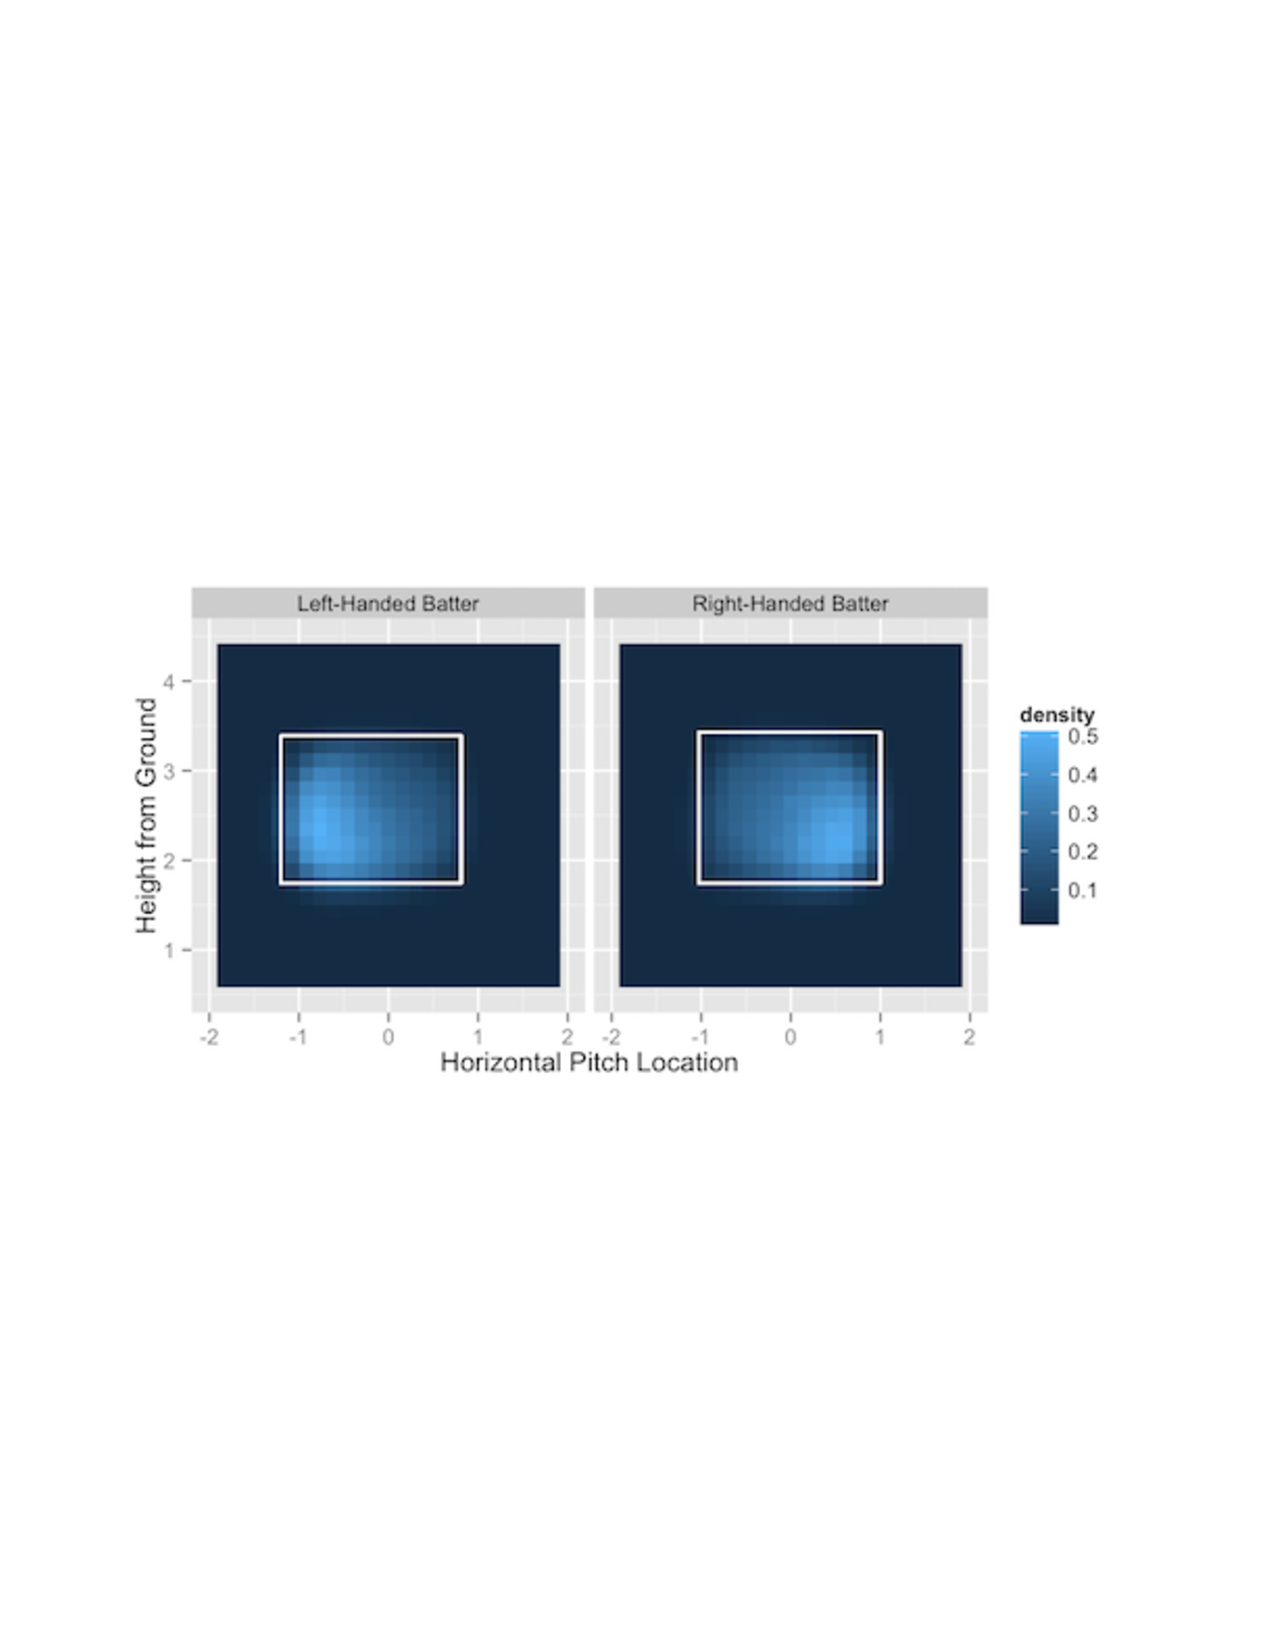
\includegraphics[width=13.54in]{images/strikes} \caption{Density of called strikes for right-handed batters and left-handed batters (from 2008 to 2013).}\label{fig:STRIKES}
\end{figure}

Figure \ref{fig:STRIKES} shows one static rectangle (or strike-zone) per
plot automatically generated by \texttt{strikeFX}. The definition of the
strike-zone is notoriously ambiguous. As a result, the boundaries of the
strike-zone may be noticeably different in some situations. However, we
can achieve a fairly accurate representation of strike-zones using a
rectangle defined by batters' average height and stance (Fast
\protect\hyperlink{ref-Strikezones}{2011}). As Figure
\ref{fig:strike-probs} reinforces, batter stance makes an important
difference since the strike-zone seems to be horizontally shifted away
from the batter. The batter's height is also important since the
strike-zone is classically defined as approximately between the batter's
knees and armpits.

Figure \ref{fig:STRIKES} has is one strike-zone per plot since the
\texttt{layer} option contains a \textbf{ggplot2} argument that facets
according to batter stance. Facet layers are a powerful tool for
analyzing PITCHf/x data because they help produce quick and insightful
comparisons. In addition to using the \texttt{layer} option, one can add
layers to a graphic returned by \texttt{strikeFX} using \textbf{ggplot2}
arithmetic. It is also worth pointing out that Figure \ref{fig:STRIKES}
could have been created without introducing the \texttt{strikes} data
frame by using the \texttt{density1} and \texttt{density2} options.

\begin{Shaded}
\begin{Highlighting}[]
\KeywordTok{strikeFX}\NormalTok{(decisions, }\DataTypeTok{geom =} \StringTok{"raster"}\NormalTok{, }\DataTypeTok{density1 =} \KeywordTok{list}\NormalTok{(}\DataTypeTok{des =} \StringTok{"Called Strike"}\NormalTok{),          }
  \DataTypeTok{density2 =} \KeywordTok{list}\NormalTok{(}\DataTypeTok{des =} \StringTok{"Called Strike"}\NormalTok{)) +}\StringTok{ }\KeywordTok{facet_grid}\NormalTok{(. ~}\StringTok{ }\NormalTok{stand, }\DataTypeTok{labeller =} \NormalTok{relabel)}
\end{Highlighting}
\end{Shaded}

In general, when \texttt{density1} and \texttt{density2} are identical,
the result is equivalent to subsetting the data frame appropriately
beforehand. More importantly, by specifying \emph{different} values for
\texttt{density1} and \texttt{density2}, differenced densities are
easily generated. In this case, a grid of density estimates for
\texttt{density2} are subtracted from the corresponding grid of density
estimates for \texttt{density1}. Note that the default \texttt{NULL}
value for either density option infers that the entire data set defines
the relevant density. Thus, if \texttt{density2} was \texttt{NULL} (when
\texttt{density1 = list(des = 'Called Strike')}), we would obtain the
density of called strikes minus the density of \emph{both} called
strikes and balls. In Figure \ref{fig:strikesVSballs}, we define
\texttt{density1} as called strikes and define \texttt{density2} as
balls. As expected, we see positive density values (in blue) inside the
strike-zone and negative density values (in red) outside of the
strike-zone.

\begin{Shaded}
\begin{Highlighting}[]
\KeywordTok{strikeFX}\NormalTok{(decisions, }\DataTypeTok{geom =} \StringTok{"raster"}\NormalTok{, }\DataTypeTok{density1 =} \KeywordTok{list}\NormalTok{(}\DataTypeTok{des =} \StringTok{"Called Strike"}\NormalTok{), }
  \DataTypeTok{density2 =} \KeywordTok{list}\NormalTok{(}\DataTypeTok{des =} \StringTok{"Ball"}\NormalTok{), }\DataTypeTok{layer =} \KeywordTok{facet_grid}\NormalTok{(. ~}\StringTok{ }\NormalTok{stand, }\DataTypeTok{labeller =} \NormalTok{relabel)) }
\end{Highlighting}
\end{Shaded}

\begin{figure}[htbp]
\centering
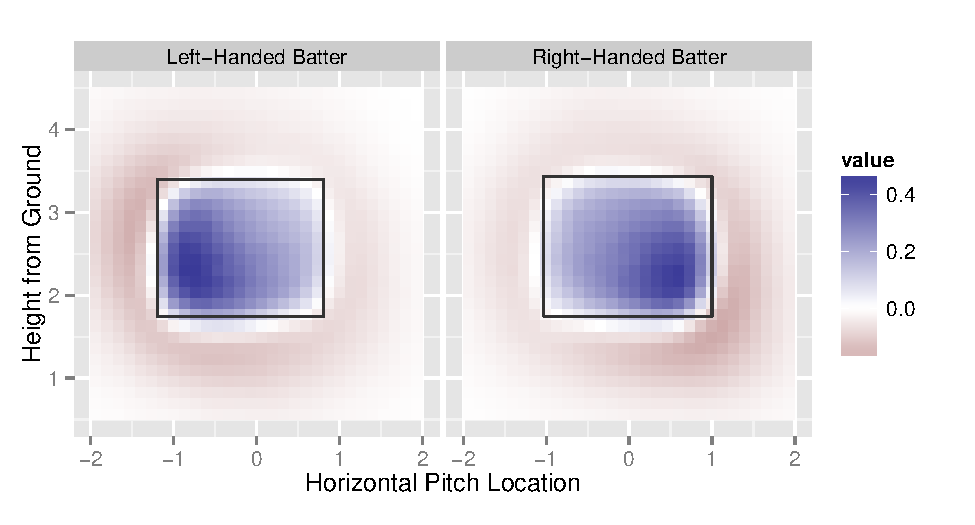
\includegraphics{images/strikesVSballs.pdf}
\caption{\label{fig:strikesVSballs}Density of called strikes minus density
of balls for both right-handed batters and left-handed batters (from
2008 to 2013). The blue region indicates a higher frequency of called
strikes and the red region indicates a higher frequency of balls.}
\end{figure}

These density plots are helpful for visualizing the observed frequency
of events; however, they are not very useful for addressing our umpire
bias hypothesis. Instead of looking simply at the \emph{density}, we
want to model the \emph{probability} of a strike called at each
coordinate given the umpire has to make a decision.

\subsubsection{Probabilistic plots}

There are many approaches to probabilistic modeling over a two
dimensional spatial region. Since our response is often categorical,
generalized additive models (GAMs) is a popular and desirable approach
to modeling events over the strike-zone (Mills
\protect\hyperlink{ref-loess}{2010}). There are numerous R package
implementations of GAMs, but the \texttt{bam} function from the
\textbf{mgcv} package has several desirable properties (Wood
\protect\hyperlink{ref-mgcv}{2006}). Most importantly, the smoothing
parameter can be estimated using several different methods. In order to
have a reasonable estimate of the smooth 2D surface, GAMs require fairly
large amount of observations. As a result, run time can be an issue --
especially when modeling 2.5 million observations! Thankfully, the
\texttt{bam} function has a \texttt{cluster} argument which allows one
to distribute computations across multiple cores using the built in
\textbf{parallel} package.

\begin{Shaded}
\begin{Highlighting}[]
\KeywordTok{library}\NormalTok{(parallel) }
\NormalTok{cl <-}\StringTok{ }\KeywordTok{makeCluster}\NormalTok{(}\KeywordTok{detectCores}\NormalTok{() -}\StringTok{ }\DecValTok{1}\NormalTok{)}
\KeywordTok{library}\NormalTok{(mgcv) }
\NormalTok{m <-}\StringTok{ }\KeywordTok{bam}\NormalTok{(strike ~}\StringTok{ }\KeywordTok{interaction}\NormalTok{(stand, p_throws, inning_side) +}\StringTok{                }
\StringTok{  }\KeywordTok{s}\NormalTok{(px, pz, }\DataTypeTok{by =} \KeywordTok{interaction}\NormalTok{(stand, p_throws, inning_side)),              }
  \DataTypeTok{data =} \NormalTok{decisions, }\DataTypeTok{family =} \KeywordTok{binomial}\NormalTok{(}\DataTypeTok{link =} \StringTok{'logit'}\NormalTok{), }\DataTypeTok{cluster =} \NormalTok{cl)}
\end{Highlighting}
\end{Shaded}

This formula models the probability of a strike as a function of the
baseball's spatial location, the batter's stance, the pitcher's throwing
arm, and the side of the inning. Since home pitchers always pitch during
the top of the inning, \texttt{inning\_side} also serves as an
indication of whether a pitch is thrown by a home pitcher. In this case,
the \texttt{interaction} function creates a factor with eight different
levels since every input factor has two levels. Consequently, there are
8 different levels of smooth surfaces over the spatial region defined by
\texttt{px} and \texttt{pz}.

The fitted model \texttt{m} contains a lot of information which
\texttt{strikeFX} uses in conjunction with any \textbf{ggplot2} facet
commands to infer which and how surfaces should be plotted. In
particular, the \texttt{var.summary} is used to identify model
covariates, as well their default conditioning values. In our case, the
majority of \texttt{decisions} are from right-handed pitchers and the
top of the inning. Thus, the default conditioning values are
\texttt{"top"} for \texttt{inning\_side} and \texttt{"R"} for
\texttt{p\_throws}. If different conditioning values are desired,
\texttt{var.summary} can be modified accordingly. To demonstrate, Figure
\ref{fig:strike-probs} shows 2 of the 8 possible surfaces that
correspond to a right-handed \emph{away} pitcher.

\begin{Shaded}
\begin{Highlighting}[]
\NormalTok{away <-}\StringTok{ }\KeywordTok{list}\NormalTok{(}\DataTypeTok{inning_side =} \KeywordTok{factor}\NormalTok{(}\StringTok{"bottom"}\NormalTok{, }\DataTypeTok{levels =} \KeywordTok{c}\NormalTok{(}\StringTok{"top"}\NormalTok{, }\StringTok{"bottom"}\NormalTok{)))}
\NormalTok{m$var.summary <-}\StringTok{ }\KeywordTok{modifyList}\NormalTok{(m$var.summary, away)}
\KeywordTok{strikeFX}\NormalTok{(decisions, }\DataTypeTok{model =} \NormalTok{m, }\DataTypeTok{layer =} \KeywordTok{facet_grid}\NormalTok{(. ~}\StringTok{ }\NormalTok{stand, }\DataTypeTok{labeller =} \NormalTok{relabel))}
\end{Highlighting}
\end{Shaded}

\begin{figure}[htbp]
\centering
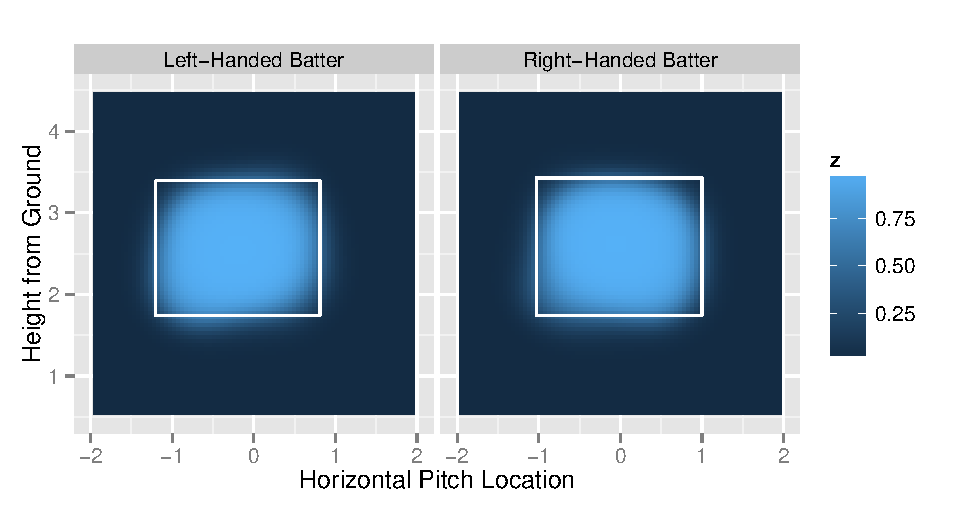
\includegraphics{images/prob-strike.pdf}
\caption{\label{fig:strike-probs}Probability that a right-handed away
pitcher receives a called strike (provided the umpire has to make a
decision). Plots are faceted by the handedness of the batter.}
\end{figure}

Using the same intuition exploited earlier to obtain differenced density
plots, we can easily obtain differenced probability plots. To obtain
Figure \ref{fig:diff-probs}, we simply add \texttt{p\_throws} as another
facet variable and \texttt{inning\_side} as a differencing variable. In
this case, conditioning values do not matter since every one of the 8
surfaces are required in order to produce Figure \ref{fig:diff-probs}.

\begin{Shaded}
\begin{Highlighting}[]
\CommentTok{# Function to create better labels for both stand and p_throws}
\NormalTok{relabel2 <-}\StringTok{ }\NormalTok{function(variable, value) \{    }
  \NormalTok{if (variable %in%}\StringTok{ "stand"}\NormalTok{)      }
    \KeywordTok{return}\NormalTok{(}\KeywordTok{sub}\NormalTok{(}\StringTok{"^L$"}\NormalTok{, }\StringTok{"Left-Handed Batter"}\NormalTok{,                 }
      \KeywordTok{sub}\NormalTok{(}\StringTok{"^R$"}\NormalTok{, }\StringTok{"Right-Handed Batter"}\NormalTok{, value)))   }
  \NormalTok{if (variable %in%}\StringTok{ "p_throws"}\NormalTok{)      }
    \KeywordTok{return}\NormalTok{(}\KeywordTok{sub}\NormalTok{(}\StringTok{"^L$"}\NormalTok{, }\StringTok{"Left-Handed Pitcher"}\NormalTok{,                 }
      \KeywordTok{sub}\NormalTok{(}\StringTok{"^R$"}\NormalTok{, }\StringTok{"Right-Handed Pitcher"}\NormalTok{, value))) }
\NormalTok{\}}
\KeywordTok{strikeFX}\NormalTok{(decisions, }\DataTypeTok{model =} \NormalTok{m, }\DataTypeTok{layer =} \KeywordTok{facet_grid}\NormalTok{(p_throws ~}\StringTok{ }\NormalTok{stand, }\DataTypeTok{labeller =} \NormalTok{relabel2),}
  \DataTypeTok{density1 =} \KeywordTok{list}\NormalTok{(}\DataTypeTok{inning_side =} \StringTok{"top"}\NormalTok{), }\DataTypeTok{density2 =} \KeywordTok{list}\NormalTok{(}\DataTypeTok{inning_side =} \StringTok{"bottom"}\NormalTok{))}
\end{Highlighting}
\end{Shaded}

\begin{figure}[htbp]
\centering
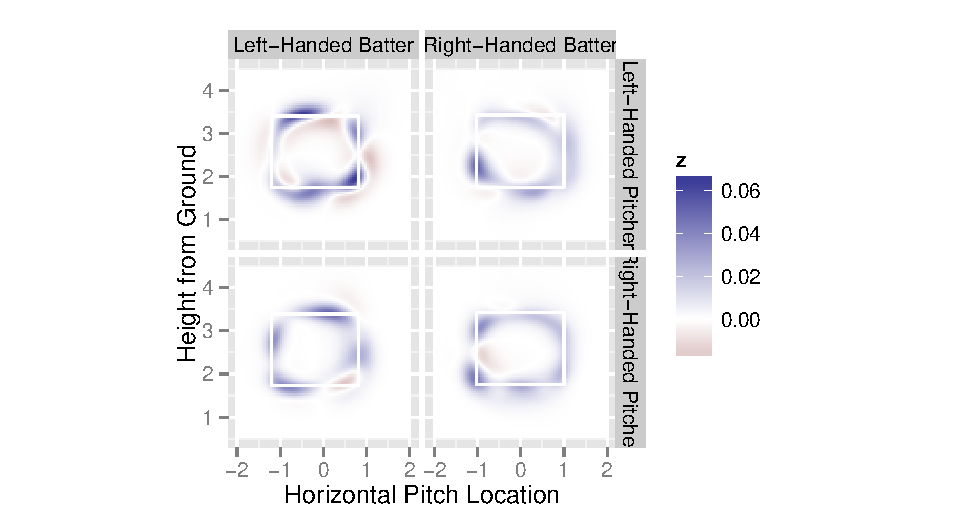
\includegraphics{images/prob-diff.pdf}
\caption{\label{fig:diff-probs}Difference between home and away pitchers in
the probability of a strike (provided the umpire has to make a
decision). The blue regions indicate a higher probability of a strike
for home pitchers and red regions indicate a higher probability of a
strike for away pitchers. Plots are faceted by the handedness of both
the pitcher and the batter.}
\end{figure}

The four different plots in Figure \ref{fig:diff-probs} represent the
four different combination of values among \texttt{p\_throws} and
\texttt{stand}. In general, provided that a pitcher throws to a batter
in the blue region, the pitch is more likely to be called a strike if
the pitcher is on their home turf. Interestingly, there is a
well-defined blue elliptical band around the boundaries of the typical
strike-zone. Thus, home pitchers are more likely to receive a favorable
call -- especially when the classification of the pitch is in question.
In some areas, the home pitcher has up to a 6 percent higher probability
of receiving a called strike than an away pitcher. The subtle
differences in spatial patterns across the different values of
\texttt{p\_throws} and \texttt{stand} are interesting as well. For
instance, pitching at home has a large positive impact for a left-handed
pitcher throwing in the lower inside portion of the strike-zone to a
right-handed batter, but the impact seems negligible in the mirror
opposite case. Differenced probabilistic densities are clearly an
interesting visual tool for analyzing PITCHf/x data. With
\texttt{strikeFX}, one can quickly and easily make all sorts of visual
comparisons for various situations. In fact, one can explore and compare
the probabilistic structure of any well-defined event over a strike-zone
region (for example, the probability a batter reaches base) using a
similar approach.

\subsection{2D animation}\label{d-animation}

\texttt{animateFX} provides convenient and flexible functionality for
animating the trajectory of any desired set of pitches. For
demonstration purposes, this section animates every four-seam and cut
fastball thrown by Mariano Rivera and Phil Hughes during the 2011
season. These pitches provide a good example of how facets play an
important role in extracting new insights. Similar methods can be used
to analyze any MLB player (or combination of players) in greater detail.

\texttt{animateFX} tracks three dimensional pitch locations over a
sequence of two dimensional plots. The animation takes on the viewpoint
of the umpire; that is, each time the plot refreshes, the balls are
getting closer to the viewer. This is reflected with the increase in
size of the points as the animation progresses. Obviously, some pitches
travel faster than others, which explains the different sizes within a
particular frame. Animations revert to the initial point of release once
\emph{all} of the baseballs have reached home plate. During an
interactive session, \texttt{animateFX} produces a series of plots that
may not viewed easily. One option available to the user is to wrap
\texttt{animation::saveHTML} around \texttt{animateFX} to view the
animation in a browser with proper looping controls (Xie
\protect\hyperlink{ref-animation}{2013}).

To reduce the time and thinking required to produce these animations,
\texttt{animateFX} has default settings for the geometry, color, opacity
and size associated with each plot. Any of these assumptions can be
altered - except for the point geometry. In order for animations to
work, a data frame with the appropriately named PITCHf/x parameters
(that is, x0, y0, z0, vx0, vy0, vz0, ax0, ay0 and az0) is required. In
Figure \ref{fig:animate1}, every four-seam and cut fastball thrown by
Rivera and Hughes during the 2011 season is visualized using the
\texttt{pitches} data frame obtained earlier (the animation is available
at \url{http://cpsievert.github.io/pitchRx/ani1}).

\begin{Shaded}
\begin{Highlighting}[]
\KeywordTok{animateFX}\NormalTok{(pitches, }\DataTypeTok{layer=}\KeywordTok{list}\NormalTok{(}\KeywordTok{theme_bw}\NormalTok{(), }\KeywordTok{coord_equal}\NormalTok{(),}
  \KeywordTok{facet_grid}\NormalTok{(pitcher_name~stand, }\DataTypeTok{labeller =} \NormalTok{relabel)))}
\end{Highlighting}
\end{Shaded}

\begin{figure}[htbp]
\centering
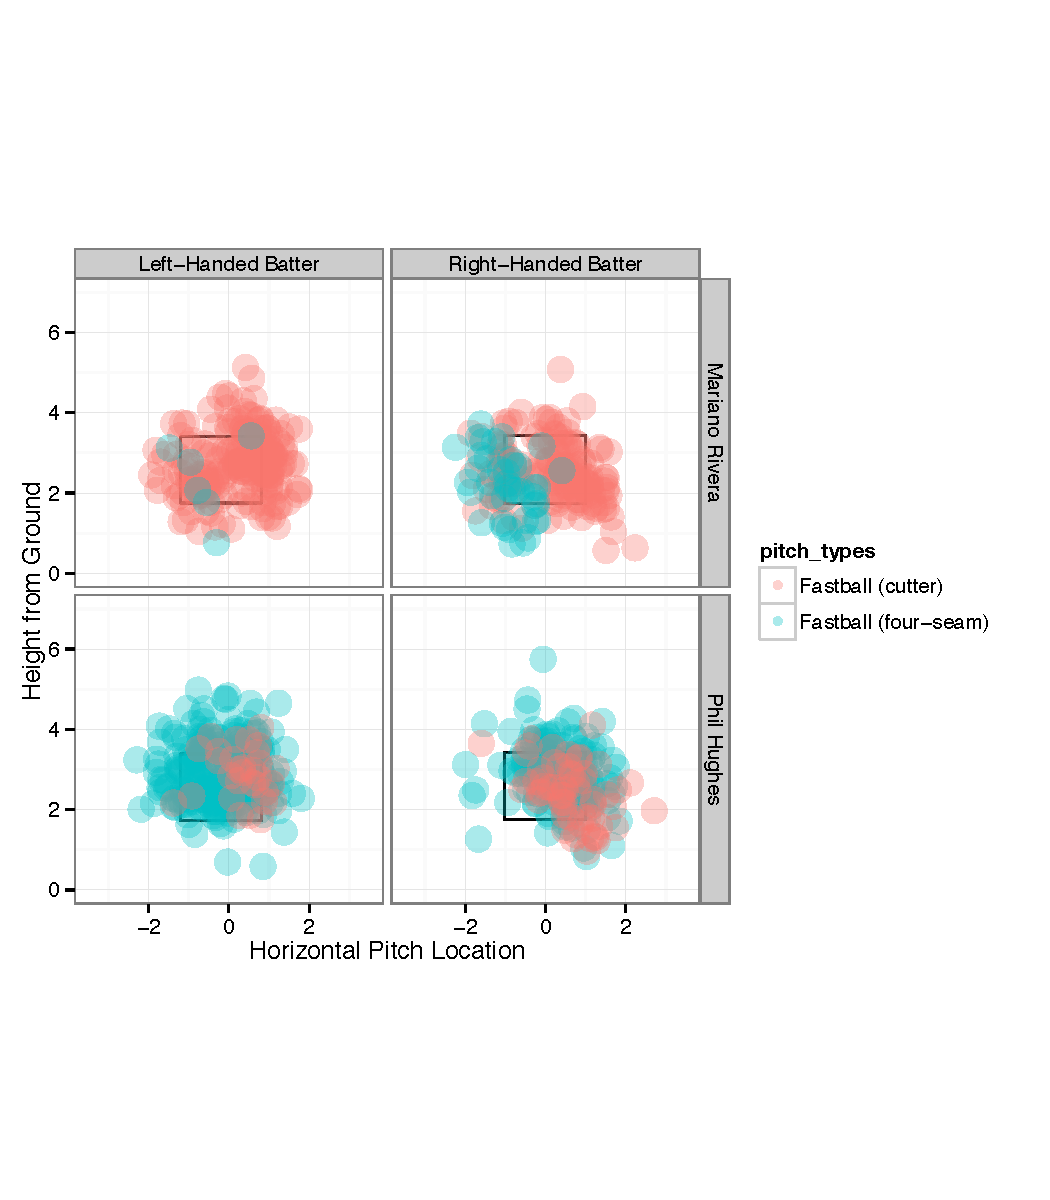
\includegraphics{images/ani-frame1.pdf}
\caption{\label{fig:animate1}The last frame of an animation of every
four-seam and cutting fastballs thrown by NY Yankee pitchers Mariano
Rivera and Phil Hughes during the 2011 season. The actual animation can
be viewed at \url{http://cpsievert.github.io/pitchRx/ani1}. Pitches are
faceted by pitcher and batting stance. For instance, the top left plot
portrays pitches thrown by Rivera to left-handed batters.}
\end{figure}

In the animation corresponding to Figure \ref{fig:animate1}, the upper
right-hand portion (Rivera throwing to right-handed batters) reveals the
clearest pattern in flight trajectories. Around the point of release,
Rivera's two pitch types are hard to distinguish. However, after a
certain point, there is a very different flight path among the two pitch
types. Specifically, the drastic left-to-right movement of the cut
fastball is noticeably different from the slight right-to-left movement
of the four-seam fastball. In recent years, cut fastballs have gained
notoriety among the baseball community as a coveted pitch for pitchers
have at their disposal. This is largely due to the difficulty that a
batter has in distinguishing the cut fastball from another fastball as
the ball travels toward home plate. Clearly, this presents an advantage
for the pitcher since they can use deception to reduce batter's ability
to predict where the ball will cross home plate. This deception factor
combined with Rivera's ability to locate his pitches explain his
accolades as one of the greatest pitchers of all time (Traub
\protect\hyperlink{ref-NYT}{2010}).

Although we see a clear pattern in Rivera's pitches, MLB pitchers are
hardly ever that predictable. Animating that many pitches for another
pitcher can produce a very cluttered graphic which is hard to interpret
(especially when many pitch types are considered). However, we may still
want to obtain an indication of pitch trajectory over a set of many
pitches. A way to achieve this is to average over the PITCHf/x
parameters to produce an overall sense of pitch type behavior (via the
\texttt{avg.by} option). Note that the facet variables are automatically
considered indexing variables. That is, in Figure \ref{fig:animate2},
there are eight `average' pitches since there are two pitch types, two
pitchers, and two types of batting stance (the animation is available at
\url{http://cpsievert.github.io/pitchRx/ani2}).

\begin{Shaded}
\begin{Highlighting}[]
\KeywordTok{animateFX}\NormalTok{(pitches, }\DataTypeTok{avg.by =} \StringTok{"pitch_types"}\NormalTok{, }\DataTypeTok{layer =} \KeywordTok{list}\NormalTok{(}\KeywordTok{coord_equal}\NormalTok{(), }\KeywordTok{theme_bw}\NormalTok{(),}
  \KeywordTok{facet_grid}\NormalTok{(pitcher_name~stand, }\DataTypeTok{labeller =} \NormalTok{relabel)))}
\end{Highlighting}
\end{Shaded}

\begin{figure}[htbp]
\centering
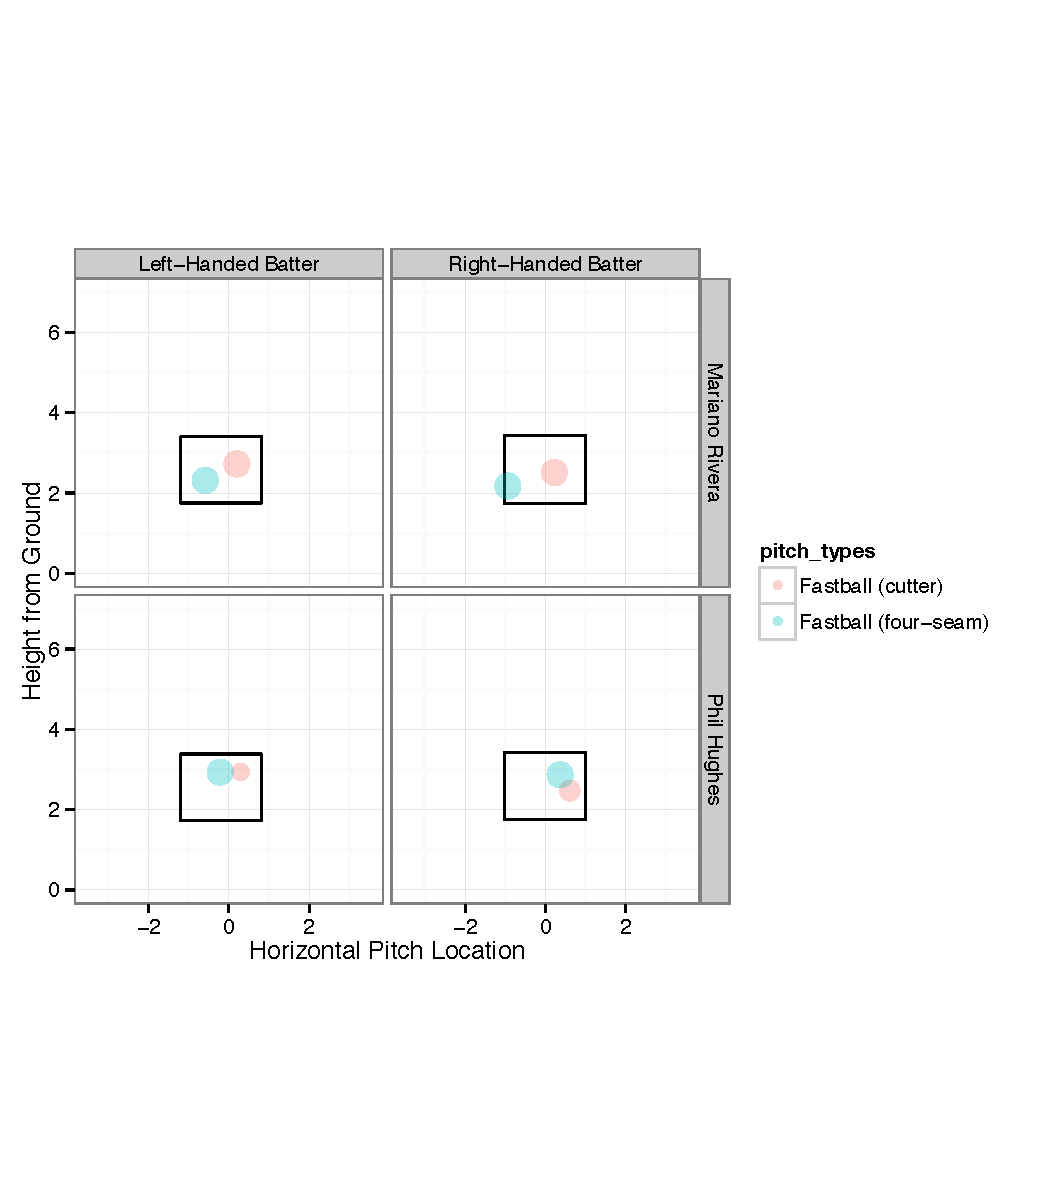
\includegraphics{images/ani-frame2.pdf}
\caption{\label{fig:animate2}The last frame of an animation of averaged
four-seam and cutting fastballs thrown by NY Yankee pitchers Mariano
Rivera and Phil Hughes during the 2011 season. The actual animation can
be viewed at \url{http://cpsievert.github.io/pitchRx/ani2}. PITCHf/x
parameters are averaged over pitch type, pitcher and batting stance. For
instance, the bottom right plot portrays an average four-seam and
average cutter thrown by Hughes to right-handed batters.}
\end{figure}

\subsection{Interactive 3D graphics}\label{interactive-3d-graphics}

\textbf{rgl} is an R package that utilizes OpenGL for graphics
rendering. \texttt{interactiveFX} utilizes \textbf{rgl} functionality to
reproduce flight paths on an interactive 3D platform. Figure
\ref{fig:rgl} has two static pictures of Mariano Rivera's 2011 fastballs
on this interactive platform. This is great for gaining new perspectives
on a certain set of pitches, since the trajectories can be viewed from
any angle. Figure \ref{fig:rgl} showcases the difference in trajectory
between Rivera's pitch types.

\begin{Shaded}
\begin{Highlighting}[]
\NormalTok{Rivera <-}\StringTok{ }\KeywordTok{subset}\NormalTok{(pitches, pitcher_name ==}\StringTok{ "Mariano Rivera"}\NormalTok{)}
\KeywordTok{interactiveFX}\NormalTok{(Rivera, }\DataTypeTok{avg.by =} \StringTok{"pitch_types"}\NormalTok{)}
\end{Highlighting}
\end{Shaded}

\begin{figure}
\includegraphics[width=11.9in]{images/rgl} \caption{3D scatterplot of pitches from Rivera. Pitches are plotted every one-hundredth of a second. Cutting fastballs are shown in red and four-seam fastballs are shown in blue. The left hand plot takes a viewpoint of Rivera and the right hand plot takes a viewpoint near the umpire. Note these are static pictures of an interactive object.}\label{fig:rgl}
\end{figure}

\section{Conclusion}\label{conclusion}

\textbf{pitchRx} utilizes \textbf{XML2R}'s convenient framework for
manipulating XML content in order to provide easy access to PITCHf/x and
related Gameday data. \textbf{pitchRx} removes access barriers which
allows the average R user and baseball fan to spend their valuable time
analyzing Gameday's enormous source of baseball information.
\textbf{pitchRx} also provides a suite of functions that greatly reduce
the amount of work involved to create popular PITCHf/x graphics. For
those interested in obtaining other XML data, \textbf{pitchRx} serves as
a nice example of leveraging \textbf{XML2R} to quickly assemble custom
XML data collection mechanisms.

\chapter{LDAvis: A method for visualizing and interpreting topics}

This chapter is a paper published in The Proceedings of the Workshop on
Interactive Language Learning, Visualization, and Interfaces (ACL 2014)
{[}Sievert:2014b{]}. I am the primary author of the paper which is
avaliable online here
\url{http://nlp.stanford.edu/events/illvi2014/papers/sievert-illvi2014.pdf}

The formatting of paper has been modified to make for consistent
typesetting across the thesis.

\specialchapt{ABSTRACT}

We present \texttt{LDAvis}, an \texttt{R} package for creating We
present \texttt{LDAvis}, a web-based interactive visualization of topics
estimated using Latent Dirichlet Allocation that is built using a
combination of R and d3. Our visualization provides a global view of the
topics (and how they differ from each other), while at the same time
allowing for a deep inspection of the tokens most highly associated with
each individual topic. First, we propose a novel method for choosing
which tokens to present to a user to aid in the task of topic
interpretation, in which we define the \emph{relevance} of a token to a
topic. Second, we present the results of a user study that illustrates
how ranking tokens by their relevance to a given topic relates to that
topic's interpretability, and we recommend a default method of computing
relevance to maximize topic interpretability. Last, we incorporate
relevance into \texttt{LDAvis} in a way that allows users to flexibly
explore topic-token relationships to better understand a fitted LDA
model.

\section{Introduction}\label{section:introduction}

Recently much attention has been paid to visualizing the output of topic
models fit using Latent Dirichlet Allocation (LDA) (Matthew J. Gardner
and Seppi \protect\hyperlink{ref-Gardner}{2010}); (Chaney and Blei
\protect\hyperlink{ref-Blei-2012}{2012}); (Jason Chuang and Heer 2012b);
(Brynjar Gretarsson and Smyth \protect\hyperlink{ref-Gretarsson}{2011}).
Such visualizations are challenging to create because of the high
dimensionality of the fitted model -- LDA is typically applied to
thousands of documents, which are modeled as mixtures of dozens of
topics, which themselves are modeled as distributions over thousands of
tokens (David M. Blei and Jordan
\protect\hyperlink{ref-Blei-2003}{2012}); (Griffiths and Steyvers
\protect\hyperlink{ref-Griffiths}{2004}). The most promising basic
technique for creating LDA visualizations that are both compact and
thorough is \emph{interactivity}.

We introduce an interactive visualization system that we call
\texttt{LDAvis} that attempts to answer a few basic questions about a
fitted topic model: (1) What is the meaning of each topic?, (2) How
prevalent is each topic?, and (3) How do the topics relate to each
other? Different visual components answer each of these questions, some
of which are original, and some of which are borrowed from existing
tools.

Our visualization (illustrated in Figure \ref{fig:overview}) has two
basic pieces. First, the left panel of our visualization presents a
``global'' view of the topic model, and answers questions 2 and 3. In
this view, we plot the topics as circles in the two-dimensional plane
whose centers are determined by computing the distance between topics
(using a distance measure of the user's choice) and then by using
multidimensional scaling to project the inter-topic distances onto two
dimensions, as is done in (Jason Chuang and Heer 2012a). We encode each
topic's overall prevalence using the areas of the circles, where we sort
the topics in decreasing order of prevalence.

Second, the right panel of our visualization depicts a horizontal
barchart whose bars represent the individual tokens that are the most
useful for interpreting the currently selected topic on the left, and
allows users to answer question 1, ``What is the meaning of each
topic?''. A pair of overlaid bars represent both the corpus-wide
frequency of a given token as well as the topic-specific frequency of
the token, as in (Jason Chuang and Heer 2012b).

The left and right panels of our visualization are linked such that
selecting a topic (on the left) reveals the most useful tokens (on the
right) for interpreting the selected topic. In addition, selecting a
token (on the right) reveals the conditional distribution over topics
(on the left) for the selected token. This kind of linked selection
allows users to examine a large number of topic-token relationships in a
compact manner.

\begin{figure}
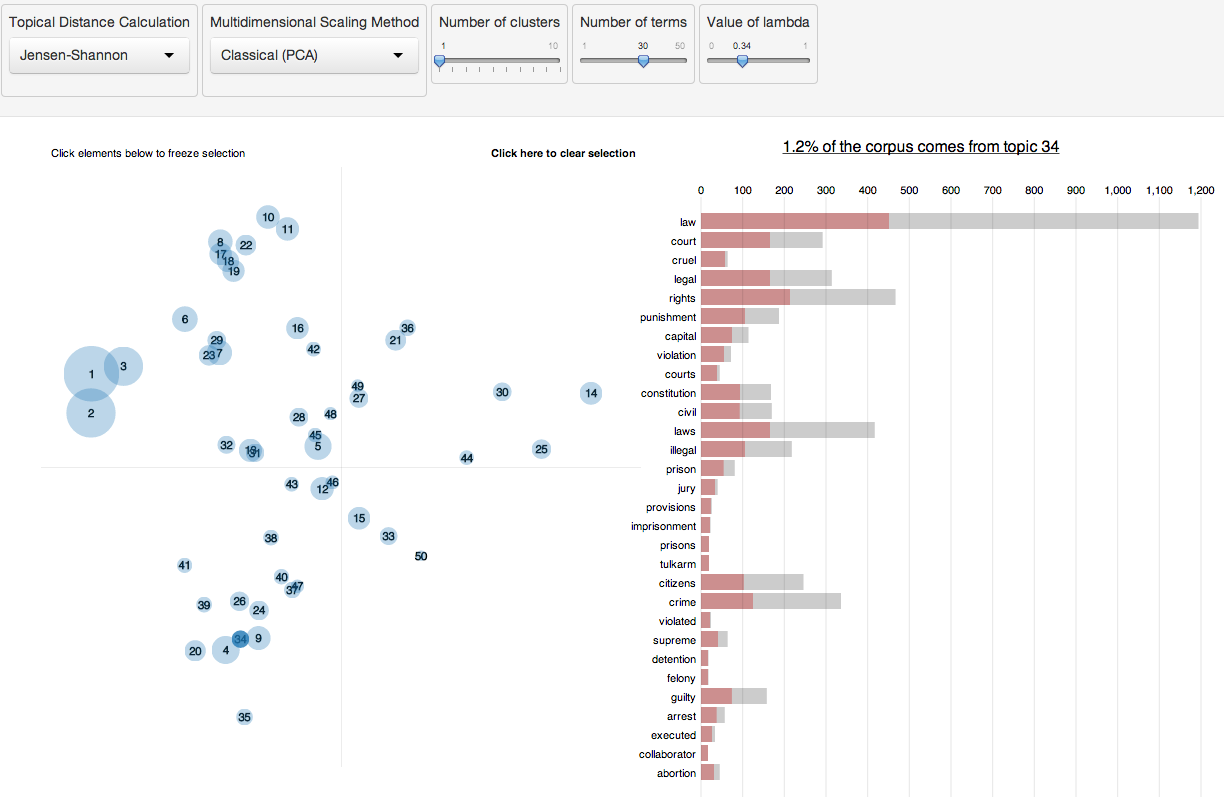
\includegraphics[width=17in]{images/fig_topic34} \caption{The layout of LDAvis, with the global topic view on the left, and the token barcharts on the right. Linked selections allow users to reveal aspects of the topic-token relationships compactly.}\label{fig:overview}
\end{figure}

A key innovation of our system is how we determine the most useful
tokens for interpreting a given topic, and how we allow users to
interactively adjust this determination. A topic in LDA is a multinomial
distribution over the tokens in the vocabulary, where the vocabulary
typically contains thousands of tokens. To interpret a topic, one
typically examines a ranked list of the most probable tokens in that
topic, using anywhere from three to thirty tokens in the list. The
problem with interpreting topics this way is that common tokens in the
corpus often appear near the top of such lists for multiple topics,
making it hard to differentiate the meanings of these topics.

Bischof and Airoldi (\protect\hyperlink{ref-Bischof}{2012}) propose
ranking tokens for a given topic in terms of both the \emph{frequency}
of the token under that topic as well as the token's \emph{exclusivity}
to the topic, which accounts for the degree to which it appears in that
particular topic to the exclusion of others. We propose a similar
measure that we call the \emph{relevance} of a token to a topic to
create a flexible method for ranking tokens in order of usefulness for
interpreting topics. We discuss our definition of relevance, and its
graphical interpretation, in detail in Section \ref{section:relevance}.
We also present the results of a user study conducted to determine the
optimal tuning parameter in the definition of relevance to aid the task
of topic interpretation in
Section\textasciitilde{}\ref{section:userstudy}, and we describe how we
incorporate relevance into our interactive visualization in
Section\textasciitilde{}\ref{section:system}.

\section{Related Work}\label{section:relatedwork}

Much work has been done recently regarding the interpretation of topics
(i.e.~measuring topic ``coherence'') as well as visualization of topic
models.

\subsection{Topic Interpretation and Coherence}

It is well-known that the topics inferred by LDA are not always easily
interpretable by humans. Jonathan Chang and Blei
(\protect\hyperlink{ref-Chang}{2009}) established via a large user study
that standard quantitative measures of fit, such as those summarized by
Hanna M. Wallach and Mimno (\protect\hyperlink{ref-Wallach}{2009}), do
not necessarily agree with measures of topic interpretability by humans.
Daniel Ramage et al. (\protect\hyperlink{ref-Ramage}{2009}) assert that
``characterizing topics is hard'' and describe how using the top-\(k\)
tokens for a given topic might not always be best, but offer few
concrete alternatives.

Loulwah AlSumait and Domeniconi
(\protect\hyperlink{ref-AlSumait}{2009}), David Mimno and McCallum
(\protect\hyperlink{ref-Mimno}{2011}), and Jason Chuang and Heer (2013b)
develop quantitative methods for measuring the interpretability of
topics based on experiments with data sets that come with some notion of
topical ground truth, such as document metadata or expert-created topic
labels. These methods are useful for understanding, in a global sense,
which topics are interpretable (and why), but they don't specifically
attempt to aid the user in interpreting \emph{individual} topics.

Blei and Lafferty (\protect\hyperlink{ref-Blei-2009}{2009}) developed
``Turbo Topics'', a method of identifying n-grams within LDA-inferred
topics that, when listed in decreasing order of probability, provide
users with extra information about the usage of tokens within topics.
This two-stage process yields good results on experimental data,
although the resulting output is still simply a ranked list containing a
mixture of tokens and n-grams, and the usefulness of the method for
topic interpretation was not tested in a user study.

David Newman and Baldwin (\protect\hyperlink{ref-Newman-JCDL}{2010})
describe a method for ranking tokens within topics to aid
interpretability called Pointwise Mutual Information (PMI) ranking.
Under PMI ranking of tokens, each of the ten most probable tokens within
a topic are ranked in decreasing order of approximately how often they
occur in close proximity to the nine other most probable tokens from
that topic in some large, external ``reference'' corpus, such as
Wikipedia or Google n-grams. Although this method correlated highly with
human judgments of token importance within topics, it does not easily
generalize to topic models fit to corpora that don't have a readily
available external source of word co-occurrences.

In contrast, Taddy (\protect\hyperlink{ref-Taddy}{2011}) uses an
intrinsic measure to rank tokens within topics: a quantity called
\emph{lift}, defined as the ratio of a token's probability within a
topic to its marginal probability across the corpus. This generally
decreases the rankings of globally frequent tokens, which can be
helpful. We find that it can be noisy, however, by giving high rankings
to very rare tokens that occur in only a single topic, for instance.
While such tokens may contain useful topical content, if they are very
rare the topic may remain difficult to interpret.

Finally, Bischof and Airoldi (\protect\hyperlink{ref-Bischof}{2012})
propose and implement a new statistical topic model that infers both a
token's frequency as well as its \emph{exclusivity} -- the degree to
which its occurrences are limited to only a few topics. They introduce a
univariate measure called a FREX score (``\(\mathbf{FR}\)equency and
\(\mathbf{EX}\)clusivity'') which is a weighted harmonic mean of a
token's rank within a given topic with respect to frequency and
exclusivity, and they recommend it as a way to rank tokens to aid topic
interpretation. We propose a similar method that is a weighted average
of a token's probability and its lift, and we justify it with a user
study and incorporate it into our interactive visualization.

\subsection{Topic Model Visualization Systems}

A number of visualization systems for topic models have arisen in recent
years. Several of them focus on allowing users to browse documents,
topics, and tokens to learn about the relationships between these three
canonical topic model units (Matthew J. Gardner and Seppi
\protect\hyperlink{ref-Gardner}{2010}); (Chaney and Blei
\protect\hyperlink{ref-Blei-2012}{2012}) (Justin Snyder and Wolfe
\protect\hyperlink{ref-Snyder}{2013}). These browsers typically use
lists of the most probable tokens within topics to summarize the topics,
and the visualization elements are limited to barcharts or word clouds
of token probabilities for each topic, pie charts of topic probabilities
for each document, and/or various barcharts or scatterplots related to
document metadata. Although these tools can be useful for browsing a
corpus, we seek a more compact visualization, with the more narrow focus
of quickly and easily understanding the individual topics themselves
(without necessarily visualizing documents).

Jason Chuang and Heer (2012b) develop such a tool, called ``Termite'',
which visualizes the set of topic-token distributions estimated in LDA
using a matrix layout. The authors introduce two measures of the
usefulness of tokens for understanding a topic model:
\emph{distinctiveness} and \emph{saliency}. These quantities measure how
much information a token conveys about a topic by computing the
Kullback-Liebler divergence between the distribution of topics given the
token and the marginal distribution of topics (distinctiveness),
optionally weighted by the token's overall frequency (saliency). The
authors recommend saliency as a thresholding method for selecting which
tokens are included in the visualization, and they further use a
seriation method for ordering the most salient tokens to highlight
differences between topics.

Termite is a compact, intuitive interactive visualization of the topics
in a topic model, but by only including tokens that rank high in
saliency or distinctiveness, which are \emph{global} properties of
tokens, it is restricted to providing a \emph{global} view of the model,
rather than allowing a user to deeply inspect individual topics by
visualizing a potentially different set of tokens for every single
topic. In fact, Jason Chuang and Heer (2013a) describe the use of a
``topic-specific word ordering'' as potentially useful future work.

\section{Relevance of tokens to topics}

Here we define \emph{relevance}, our method for ranking tokens within
topics, and we describe the results of a user study to learn an optimal
tuning parameter in the computation of relevance.

\subsection{Definition of Relevance}\label{section:relevance}

Let \(\phi_{kw}\) denote the probability of token
\(w \in \{1, ..., V\}\) for topic \(k\in \{1, ..., K\}\), where \(V\)
denotes the number of unique tokens in the vocabulary, and let \(p_w\)
denote the marginal probability of token \(w\) in the corpus. One
typically estimates \(\phi\) in LDA using Variational Bayes methods or
Collapsed Gibbs Sampling, and \(p_w\) from the empirical distribution of
the corpus (optionally smoothed by including prior weights as
pseudo-counts).

We define the \emph{relevance} of token \(w\) to topic \(k\) given a
weight parameter \(\lambda\) (where \(0 \leq \lambda \leq 1\)) as: \[
r(w, k \mid \lambda) = \lambda \log(\phi_{kw}) + (1 - \lambda)\log\Bigl(\frac{\phi_{kw}}{p_w}\Bigr),
\] where \(\lambda\) determines the weight given to the probability of
token \(w\) under topic \(k\) relative to its lift. Setting
\(\lambda = 1\) results in the familiar ranking of tokens in decreasing
order of their topic-specific probability, and setting \(\lambda = 0\)
ranks tokens solely by their lift, which we found anecdotally to result
in ``noisy'' topics full of rare tokens. We wish to learn an ``optimal''
value of \(\lambda\) for topic interpretation from our user study.

First, though, to see how different values of \(\lambda\) result in
different ranked token lists, consider the plot in Figure
\ref{fig:relevance}. We fit a 50-topic model to the 20 Newsgroups data
(details are described in
Section\textasciitilde{}\ref{section:userstudy}) and plotted
\(\log\)(lift) on the \(y\)-axis vs. \(\log(\phi_{kw})\) on the
\(x\)-axis for each token in the vocabulary (which has size
\(V=22,524\)) for a given topic. Figure \ref{fig:relevance} shows this
plot for Topic 29, which occurred mostly in documents posted to the
``Motorcycles'' newsgroup, but also from documents posted to the
``Automobiles'' newsgroup and the ``Electronics'' newsgroup.
Graphically, the line separating the most relevant tokens for this
topic, given \(\lambda\), has slope \(-\lambda/(1 - \lambda)\) (see
Figure \ref{fig:relevance}).

For this topic, the top-5 most relevant tokens given \(\lambda = 1\)
(ranking solely by probability) are \{out, \#emailaddress,
\#twodigitnumer, up, \#onedigitnumber\}, where a `\#' symbol denotes a
token that is an entity representing a class of things. In contrast to
this list, which contains globally common tokens and which provides very
little meaning regarding motorcycles, automobiles, or electronics, the
top-5 most relevant tokens given \(\lambda = 1/3\) are \{oil, plastic,
pipes, fluid, and lights\}. The second set of tokens is much more
descriptive of the topic being discussed than the first.

\begin{figure}[htbp]
\centering
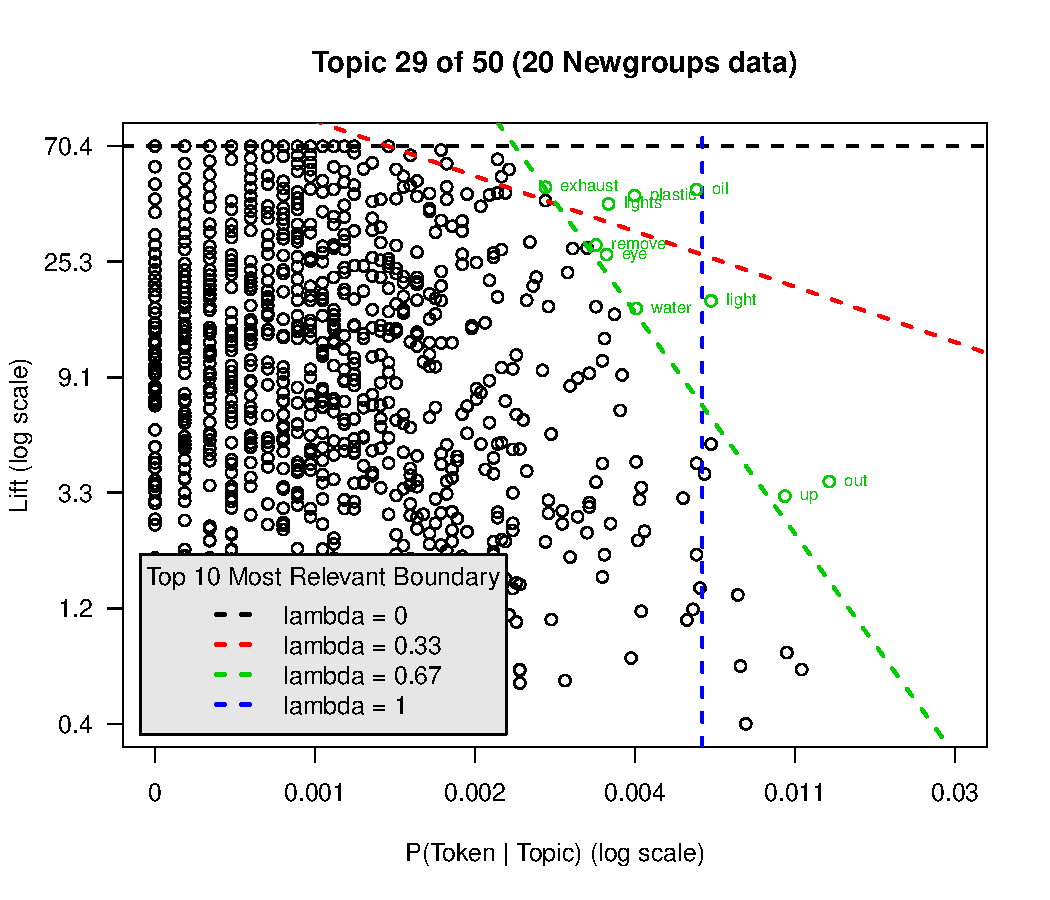
\includegraphics{images/fig_topic29.pdf}
\caption{\label{fig:relevance}Dotted lines separating the top-10 most
relevant tokens for different values of \(\lambda\), with the most
relevant tokens for \(\lambda\) = 2/3 displayed and highlighted in
green.}
\end{figure}

\subsection{User Study}\label{section:userstudy}

We conducted a user study to determine whether there was an optimal
value of \(\lambda\) in the definition of relevance to aid topic
interpretation. First, we fit a 50-topic model to the \(D=13,695\)
documents in the 20 Newsgroups data which were posted to a single
Newsgroup (rather than two or more Newsgroups). We used the Collapsed
Gibbs Sampler algorithm (Griffiths and Steyvers
\protect\hyperlink{ref-Griffiths}{2004}) to sample the latent topics for
each of the \(N=1,590,376\) tokens in the data, and we saved their topic
assignments from the last iteration (after convergence). We then
computed the 20 by 50 table, \(T\), which contains, in cell \(T_{gk}\),
the count of the number of times a token from topic
\(k \in \{1, ..., 50\}\) was assigned to Newsgroup
\(g \in \{1, ..., 20\}\), where we defined the Newsgroup of a token to
be the Newsgroup to which the document containing that token was posted.
Some of the LDA-inferred topics occurred almost exclusively (\(>90\)\%
of occurrences) in documents from a single Newsgroup, such as Topic 38,
which was the estimated topic for 15,705 tokens in the corpus, 14,233 of
which came from documents posted to the ``Medicine'' (or ``sci.med'')
Newsgroup. Other topics occurred in a wide variety of Newsgroups. One
would expect these ``spread-out'' topics to be harder to interpret than
the ``pure'' topics like Topic 38.

In the study we recruited 29 subjects among our colleagues, and each
subject completed an online experiment consisting of 50 tasks, one for
each topic in the fitted LDA model. Task \(k\) (for
\(k \in \{1, ..., 50\}\)) was to read a list of five tokens, ranked from
1-5 in terms of relevance to topic \(k\), where \(\lambda \in (0, 1)\)
was randomly sampled to compute relevance. The user was instructed to
identify which ``topic'' the list of tokens discussed from a list of
three possible ``topics'', where their choices were names of the
Newsgroups. The correct answer for task \(k\) (i.e.~our ``ground
truth'') was defined as the Newsgroup that contributed the most tokens
to topic \(k\) (i.e.~the Newsgroup with the largest count in the \(k\)th
column of the table \(T\)), and the two alternative choices were the
Newsgroups that contributed the second and third-most tokens to topic
\(k\).

We anticipated that the effect of \(\lambda\) on the probability of a
user making the correct choice could be different across topics. In
particular, for ``spread-out'' topics that were inherently difficult to
interpret, because their tokens were drawn from a wide variety of
Newsgroups (similar to a ``fused'' topic in Jason Chuang and Heer
(2013b)), we expected the proportion of correct responses to be roughly
1/3 no matter the value of \(\lambda\) used to compute relevance.
Similarly, for very ``pure'' topics, whose tokens were drawn almost
exclusively from one Newsgroup, we expected the task to be easy for any
value of \(\lambda\). To account for this, we analyzed the experimental
data by fitting a varying-intercepts logistic regression model to allow
each of the fifty topics to have its own baseline difficulty level,
where the effect of \(\lambda\) is shared across topics. We used a
quadratic function of \(\lambda\) in the model (linear, cubic and
quartic functions were explored and rejected).

As expected, the baseline difficulty of each topic varied widely. In
fact, seven of the topics were correctly identified by all 29 users, and
one topic was incorrectly identified by all 29 users. For the remaining
42 topics we estimated a topic-specific intercept term to control for
the inherent difficulty of identifying the topic (not just due to its
tokens being spread among multiple Newsgroups, but also to account for
the inherent familiarity of each topic to our subject pool -- subjects,
on average, were more familiar with ``Cars'' than ``The X Window
System'', for example).

\begin{figure}[htbp]
\centering
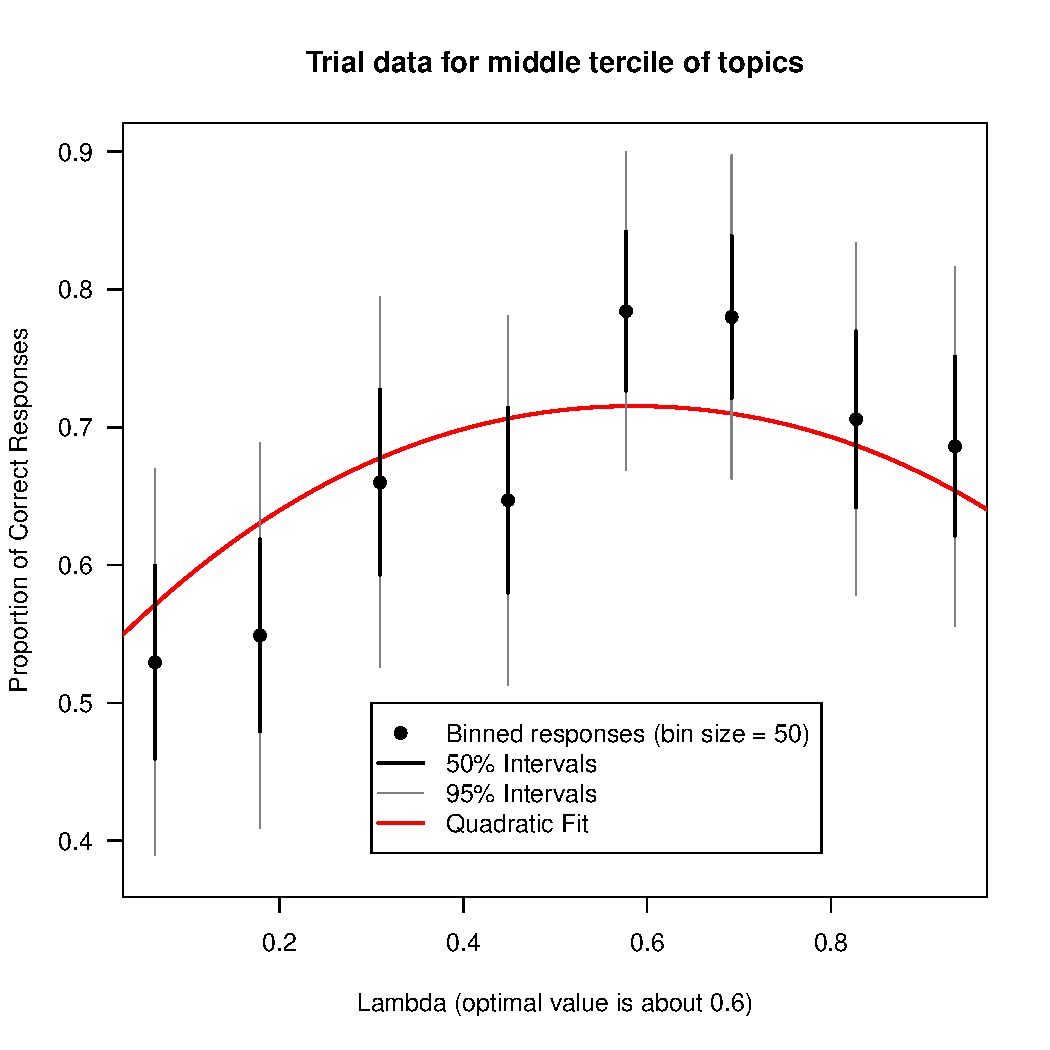
\includegraphics{images/fig_lambda.pdf}
\caption{\label{fig:lambda}A plot of the proportion of correct responses in
a user study vs.~the value of \(\lambda\) used to compute the most
relevant tokens for each topic.}
\end{figure}

The estimated effects of \(\lambda\) and \(\lambda^2\) were 2.74 and
-2.34, with standard errors 1.03 and 1.00. Taken together, their joint
effect was statistically significant (\(\chi^2\) p-value = 0.018). \%,
but the signs of their coefficients agreed with out intuition, and in a
similarly designed large-scale user study (on Mechanical Turk, for
instance), we expect that their joint effect would be statistically
significant. To see the estimated effect of \(\lambda\) on the
probability of correctly identifying a topic, consider Figure
\ref{fig:lambda}. We plot binned proportions of correct responses (on
the y-axis) vs. \(\lambda\) (on the x-axis) for the 14 topics whose
estimated topic-specific intercepts fell into the middle tercile among
the 42 topics that weren't trivial or impossible to identify. Among
these topics there was roughly a 67\% baseline probability of correct
identification. As Figure \ref{fig:lambda} shows, for these topics, the
``optimal'' value of \(\lambda\) was about 0.6, and it resulted in a
70\% - 75\% probability of correct identification, whereas for values of
\(\lambda\) near 0 or 1, the proportion of correct responses was closer
to 55\% or 60\%. We view this as evidence that ranking tokens according
to relevance, where \(\lambda < 1\), can aid topic interpretation, even
if this precise task (selecting a known topic label from a list of
pre-defined labels associated with each document as metadata) is not
always the goal. A similar conclusion might be drawn from an experiment
to study the FREX token ranking method of Bischof and Airoldi
(\protect\hyperlink{ref-Bischof}{2012}).

Note that in our experiment, we used the collection of single-posted 20
Newsgroups documents to define our ``ground truth'' data. An alternative
method for collecting ``ground truth'' data would have been to recruit
experts to label topics from an LDA model. We chose against this option
because doing so would present a classic ``chicken-or-egg'' problem: If
we use expert-labeled topics in an experiment to learn how to summarize
topics so that they can be interpreted (i.e. ``labeled''), we would only
re-learn the way that our experts were instructed, or allowed, to label
the topics in the first place! If, for instance, the experts were
presented with a ranked list of the most probable tokens for each topic,
this would influence the interpretations and labels they give to the
topics, and the experimental result would be the circular conclusion
that ranking tokens by probability allows users to recover the
``expert'' labels most easily. To avoid this, we felt strongly that we
should use data in which documents have metadata associated with them.
The 20 Newsgroups data provides an externally validated source of topic
labels, in the sense that the labels were presented to users (in the
form of Newsgroup names), and users subsequently filled in the content.
It represents, essentially, a crowd-sourced collection of tokens, or
content, for a certain set of topic labels.

\section{Our Visualization System}\label{section:system}

Our interactive, web-based visualization system, \texttt{LDAvis}, has
two core functionalities that enable users to understand the topic-token
relationships in a fitted LDA model, and a number of extra features that
provide additional perspectives on the model. \%Usually these questions
can not be answered easily with a few simple plots and/or metrics.
Instead, an interactive layout such as \texttt{LDAvis} allows one to
quickly explore model output, form new hypotheses and verify findings.

\begin{figure}[htbp]
\centering
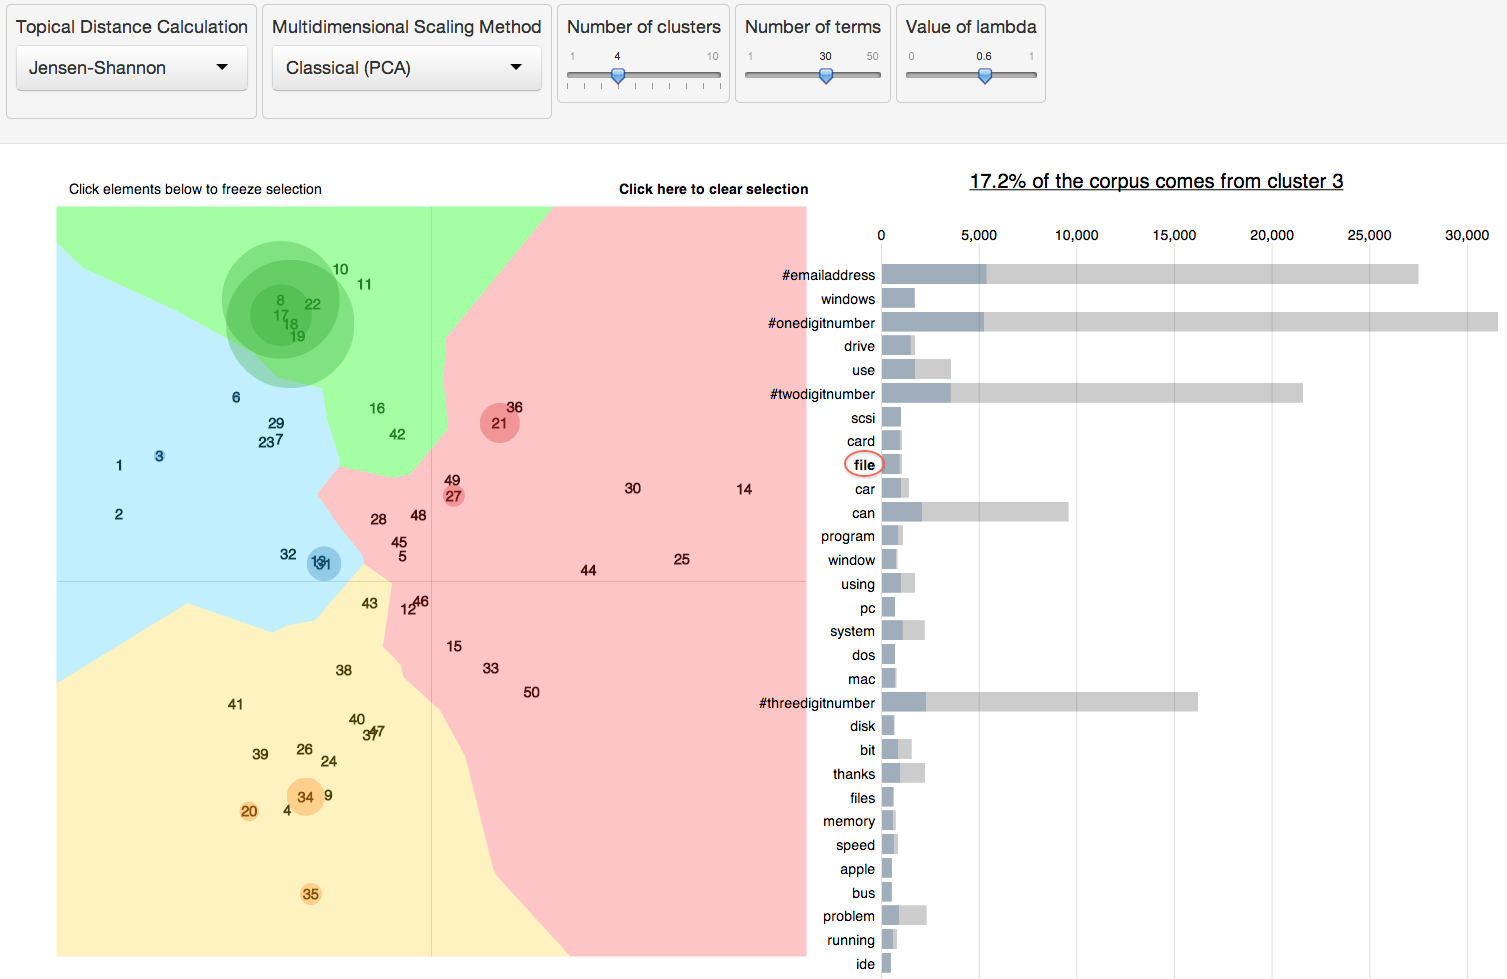
\includegraphics{images/fig_file_new2}
\caption{\label{fig:file}The user has chosen to segment the topics into four
clusters, and has selected the green cluster to populate the barchart
with the most relevant tokens for that cluster. Then, the user hovered
over the ninth bar from the top, `file', to display the conditional
distribution over topics for this token.}
\end{figure}

First and foremost, \texttt{LDAvis} allows one to select a topic to
reveal the most relevant tokens for that topic. In Figure
\ref{fig:overview}, Topic 34 is selected, and its 30 most relevant
tokens (given \(\lambda\) = 0.34, in this case) populate the bar chart
to the right (ranked in order of relevance from top to bottom). The
widths of the gray bars represent the corpus-wide frequencies of each
token, and the widths of the red bars represent the topic-specific
frequencies of each token. A slider allows users to change the value of
\(\lambda\), which can alter the rankings of tokens to aid topic
interpretation. By default, \(\lambda\) is set to 0.6, as suggested by
our user study in Section\textasciitilde{}\ref{section:userstudy}. If
\(\lambda = 1\), tokens are ranked solely by \(\phi_{kw}\), which
implies the red bars would be sorted from widest (at the top) to
narrowest (at the bottom). By comparing the widths of the red and gray
bars for a given token, users can quickly understand whether a token is
highly relevant to the selected topic because of its lift (a high ratio
of red to gray), or its probability (absolute width of red). The top 3
most relevant tokens in Figure \ref{fig:overview} are ``law'',
``rights'', and ``court''. Note that ``law'' is a common word which is
generated by Topic 34 in about 40\% of its corpus-wide occurrences,
whereas ``cruel'' is a relatively rare word with very high lift -- it
occurs almost exclusively in Topic 34. Such properties of the
topic-token relationship are readily visible in \texttt{LDAvis} for
every topic.

On the left panel, two visual features provide a global perspective of
the topics. First, the areas of the circles are proportional to the
relative prevalences of the topics in the corpus, \(\theta_k\), which
can be computed as \(\theta_k = \sum_d N_d\theta_{dk}\) for documents
\(d = 1, ..., D\), where document \(d\) contains \(N_d\) tokens. In the
50-topic model fit to the 20 Newsgroups data, the first three topics
comprise 12\%, 9\%, and 6\% of the corpus, and all contain common,
non-specific tokens (although there are differences: Topic 2 contains
formal debate-related language such as ``conclusion'', ``evidence'', and
``argument'', whereas Topic 3 contains slang conversational language
such as ``kinda'', ``like'', and ``yeah''). In addition to visualizing
topic prevalence, the left pane shows inter-topic differences. The
default for computing inter-topic distances is Jensen-Shannon
divergence, although other metrics are enabled. The default for scaling
the set of inter-topic distances defaults to Principal Components, but
other other algorithms are also enabled.

The second core feature of \texttt{LDAvis} is the ability to select a
token (by hovering over it) to reveal its conditional distribution over
topics. This distribution is visualized by altering the areas of the
topic circles such that they are proportional to the token-specific
frequencies across the corpus. This allows the user to verify, as
discussed in Jason Chuang and Heer (2012a), whether the multidimensional
scaling of topics has faithfully clustered similar topics in
two-dimensional space. For example, in Figure \ref{fig:file}, the token
``file'' is selected. In the majority of this token's occurrences, it is
drawn from one of several topics located in the upper left-hand region
of the global topic view. Upon inspection, this group of topics can be
interpreted broadly as a discussion of computer hardware and software.
This verifies, to some extent, their placement, via multidimensional
scaling, into the same two-dimensional region. It also suggests that the
word ``file'' used in this context refers to a computer file. However,
there is also conditional probability mass for the token ``file'' on
Topic 34. As shown in Figure \ref{fig:overview}, Topic 34 can be
interpreted as discussing the criminal punishment system where ``file''
refers to court filings. Similar discoveries can be made for any word
that exhibits polysemy (such as ``drive'' appearing in computer- and
automobile-related topics, or ``ground'' occurring in electrical- and
baseball-related topics).

Beyond its within-browser interaction capability, \texttt{LDAvis}
leverages the \texttt{R} language to allow users to easily alter the
topical distance measurement as well as the multidimensional scaling
algorithm to produce the global topic view. In addition, there is an
option to apply \(k\)-means clustering to the topics (as a function of
their two-dimensional locations in the global topic view). This is
merely an effort to facilitate semantic zooming in an LDA model with
many topics where `after-the-fact' clustering may be an easier way to
learn clusters of topics, rather than fitting a hierarchical topic model
(David M. Blei and Tenenbaum
\protect\hyperlink{ref-Blei-hierarchical}{2003}), for example. Selecting
a cluster (or region) of topics reveals the most relevant tokens for
that group of topics, where the token distribution of a cluster of
topics is defined as the average of the token distributions of the
individual topics in the cluster. In Figure \ref{fig:file}, the green
cluster of topics is selected, and the most relevant tokens are
predominantly related to computer hardware and software.

\section{Discussion}\label{section:futurework}

We have described a web-based, interactive visualization system,
\texttt{LDAvis}, that enables deep inspection of topic-token
relationships in an LDA model, while simultaneously providing a
``global'' view of the topics, via their prevalences and similarities to
each other, in a compact space. We also propose a novel way to rank
tokens within topics to aid in the task of topic interpretation, and we
present a user study that attempts to not only \emph{measure} the
interpretability of a topic, but also how to \emph{maximize} the
interpretability of the topic.

For future work, we anticipate performing a larger user study to further
understand how to facilitate topic interpretation in fitted LDA models,
including a comparison of multiple methods, such as ranking by Turbo
Topics (Blei and Lafferty \protect\hyperlink{ref-Blei-2009}{2009}) or
FREX scores (Bischof and Airoldi \protect\hyperlink{ref-Bischof}{2012}),
in addition to relevance. We also note the need to visualize
correlations between topics, as this can provide insight into what is
happening on the document level without actually displaying entire
documents. Last, we seek a solution to the problem of visualizing a
large number of topics (say, from 100 - 500 topics) in a compact way.

\chapter{Extending ggplot2's grammar of graphics implementation for linked and dynamic graphics on the web}

This chapter is a paper currently under revision with intention of
submitting to the Journal of Computational and Graphical Statistics. I
am the primary author of the paper and there is a working draft
available here --
\url{https://github.com/tdhock/animint-paper/blob/jcgs/HOCKING-animint.pdf}

The formatting of paper has been modified to make for consistent
typesetting across the thesis.

\specialchapt{ABSTRACT}

The web is the most popular medium for sharing interactive data
visualizations thanks to the portability of the web browser and the
accessibility of the internet. Unfortunately, creating interactive web
graphics often requires a working knowledge of numerous web technologies
that are foreign to many people working with data. As a result, web
graphics are rarely used for exploratory data analysis where quick
iteration between different visualizations is of utmost importance. This
is the core strength of ggplot2, a popular data visualization package
for R, the world's leading open-source statistical programming language.
The conceptual framework behind ggplot2 is based on the grammar of
graphics, which lays a foundation for describing any static graphic as a
small set of independent components. Perhaps the most fundamental
component is the mapping from abstract data to the visual space,
sometimes referred to as the aesthetic mapping. We propose adding two
new aesthetics to the grammar, which together are sufficient for
elegantly describing both animations and certain classes of coordinated
linked views. We implement this extension in the open-source R package
animint, which converts ggplot2 objects to interactive web
visualizations via D3.

\section{Introduction}
\label{sec:intro}

The world's leading open source statistical programming language, R, has
a rich history of interfacing with computational tools for the use of
people doing data analysis and statistics research (R Core Team
\protect\hyperlink{ref-RCore}{2015}). Understanding R's core audience is
important, as they typically want to maximize their time working on data
analysis problems, and minimize time spent learning computational tools.
R excels in this regard, as it is designed specifically for interactive
use, where users can quickly explore their data using highly expressive
interfaces. Another key player in R's success story is its packaging
infrastructure, which provides tools for distributing entire research
conpendium(s) (code, data, documentation, auxiliary documents, etc)
(Gentleman and Lang \protect\hyperlink{ref-Gentleman:Lang}{2004}).

One of the most widely used R packages is ggplot2 (Wickham
\protect\hyperlink{ref-ggplot2-book}{2009}\protect\hyperlink{ref-ggplot2-book}{b}),
a data visualization package inspired by the grammar of graphics
(Wilkinson et al. \protect\hyperlink{ref-wilkinson}{2006}). In fact,
Donoho (\protect\hyperlink{ref-Donoho:2015tu}{2015}) writes: ``This
effort may have more impact on today's practice of data analysis than
many highly-regarded theoretical statistics papers``. In our experience,
ggplot2 has made an impact thanks to its foundation in the grammar of
graphics, carefully chosen defaults, and overall usability. This helps
data analysts rapidly iterate and discover informative visualizations --
an essential task in exploratory data analysis (EDA). When dealing with
high-dimensional data, however, it is often useful to produce
interactive and/or dynamic graphics, which ggplot2 does not inherently
support.

Interactive graphics toolkits in R have been used for decades to enhance
the EDA workflow, but these approaches are often not easy to reproduce
or distribute to a larger audience. It is true that most graphics
generated during EDA are ultimately not useful, but sometimes,
understanding gained during this phase is most easily shared via the
interactive graphics themselves. Thus, there is value is being able to
easily share, and embed interactive graphics inside a larger report.
Unfortunately, this is typically hard, if not impossible, using
traditional interactive graphics toolkits. As a result, there is a large
disconnect between the visualization tools that we use for exploration
versus presentation.

We aim to narrow this gap in visualization tools by extending ggplot2's
grammar of graphics implementation for interactive and dynamic web
graphics. Our extension allows one to create animated transitions and
perform database queries via direct manipulation of linked views like
those described in (Ahlberg, Williamson, and Shneiderman
\protect\hyperlink{ref-Ahlberg:1991}{1991}) and (Buja et al.
\protect\hyperlink{ref-Buja:1991vh}{1991}). A conceptual model for our
extension is provided in Section\textasciitilde{}\ref{sec:extension} and
Section\textasciitilde{}\ref{sec:animation}. In
Section\textasciitilde{}\ref{sec:worldbank}, we demonstrate our
extension with an example. In
Section\textasciitilde{}\ref{sec:implementation}, we outline design
decisions made in our implementation in the R package animint. In
Section\textasciitilde{}\ref{sec:performance}, we provide a sense scope
for our system and its performance limitations through a handful of
examples. In Section\textasciitilde{}\ref{sec:compare}, we conduct a
comparison study by replicating examples with other leading systems.
Finally, in Section\textasciitilde{}\ref{sec:limitations}, we discuss
future work and limitations of our current system.

\section{Related Work}

We aim to provide a system which empowers ggplot2 users to go beyond the
confines of static graphics with minimal friction imposed upon their
current workflow. We acknowledge that numerous systems which support
similar visualization techniques exist outside of the R ecosystem, but
we intentionally focus on R interfaces since the surrounding statistical
computing environment is crucial for enabling an efficient exploratory
data analysis workflow.

It is important to acknowledge that ggplot2 is built on top of the R
package grid, a low-level graphics system, which is now bundled with R
itself (R Core Team \protect\hyperlink{ref-RCore}{2015}). Neither grid,
nor base R graphics, have strong support for handling user interaction
creating a need for add-on packages. There are a number of approaches
these packages take to rendering, each with their own benefits and
drawbacks. Traditionally, they build on low-level R interfaces to
graphical systems such as GTK+ (Lawrence and Temple Lang
\protect\hyperlink{ref-RGtk2}{2010}), Qt (Lawrence and Sarkar
\protect\hyperlink{ref-qtbase}{2016}\protect\hyperlink{ref-qtbase}{a});
(Lawrence and Sarkar
\protect\hyperlink{ref-qtpaint}{2016}\protect\hyperlink{ref-qtpaint}{b}),
or Java GUI frameworks (Urbanek \protect\hyperlink{ref-rJava}{2015}). In
general, the resulting system can be very fast and flexible, but sharing
ir reproducing output is usually a problem due to the heavy software
requirements. Although there may be sacrifice in performance, using the
modern web browser as a canvas is more portable, accessible, and
composable (graphics can be embedded within larger
frameworks/documents).

Base R does provide a Scalable Vector Graphics (SVG) device,
\texttt{svg()}, via the Cairo graphics API (Cairo
\protect\hyperlink{ref-cairo}{2016}). The R package SVGAnnotation (Nolan
and Temple Lang \protect\hyperlink{ref-SVGAnnotation}{2012}) provides
functionality to post-process \texttt{svg()} output in order to add
interactive and dynamic features. This is a powerful approach, since in
theory it can work with any R graphic, but the package is self described
as a proof-of-concept which reverse engineers poorly structured
\texttt{svg()} output. As a result, anyone wishing to extend or alter
the core functionality needs a deep understanding of base graphics and
SVG.

The lack of well-structured SVG for R graphics motivated the gridSVG
package which provides sensible structuring of SVG output for grid
graphics (Murrell and Potter \protect\hyperlink{ref-gridSVG}{2015}).
This package also provides some low-level tools for animating or adding
interactive features, where grid objects must be referenced by name. As
a result, if one wanted to use this interface to add interactivity to a
ggplot2 plot, they must know and understand the grid naming scheme
ggplot2 uses internally and hope it does not change down the road. An
interface where interactivity can be expressed by referencing the data
to be visualized, rather than the building blocks of the graphics
system, would be preferable since the former interface is decoupled from
the implementation and does not require knowledge of grid.

In terms of the user interface, the R package gganimate is very similar
to our system (Robinson \protect\hyperlink{ref-gganimate}{2016}). It
directly extends ggplot2 by adding a new aesthetic, named
\texttt{frame}, which splits the data into subsets (one for each unique
value of the frame variable), produces a static plot for each subset,
and uses the animation package to combine the images into a key frame
animation (Xie \protect\hyperlink{ref-animation}{2013}). This is quite
similar, but not as flexible as our system's support for animation,
which we fully describe in Section\textasciitilde{}\ref{sec:animation}.
Either system has the ability to control the amount of time that a given
frame is displayed, but our system can also animate the transition
between frames via the \texttt{d3.transition()} API (Bostock,
Oglevetsky, and Heer \protect\hyperlink{ref-d3}{2011}). Smooth
transitions help us track positions between frames, which is useful in
many scenarios, such as the touring example discussed in
Section\textasciitilde{}6.

Tours are a useful visualization technique for exploring
high-dimensional data which requires interactive and dynamic graphics.
The open source software ggobi is currently the most fully-featured tool
for touring data and has support for interactive techniques such as
linking, zooming, panning, and identifying (Cook and Swayne
\protect\hyperlink{ref-ggobi:2007}{2007}). The R package rggobi (Wickham
et al. \protect\hyperlink{ref-rggobi}{2008}) provides an R interface to
ggobi's graphical interface, but unfortunately, the software
requirements for installation and use of this toolchain are heavy and
stringent. Furthermore, sharing the interactive versions of these
graphics are not possible. The R package cranvas aims to be the
successor to ggobi, with support for similar interactive techniques, but
with a more flexible interface for describing plots inspired by the
grammar of graphics (Yihui Xie \protect\hyperlink{ref-cranvas}{2013}).
Cranvas also has heavy and stringent software requirements which limits
the portability and accessibility of the software.

Another R package for interactive graphics which draws design
inspiration from the grammar of graphics is ggvis (Chang and Wickham
\protect\hyperlink{ref-ggvis}{2015}). It does not directly extend
ggplot2, but instead provides a brand new purely functional interface
which is designed with interactive graphics in mind. It currently relies
on Vega to render the SVG graphics from JSON (Heer
\protect\hyperlink{ref-vega}{2014}), and the R package shiny to enable
many of its interactive capabilities (Chang et al.
\protect\hyperlink{ref-shiny}{2015}). The interface gives tremendous
power to R users, as it allows one to write R functions to handle user
events. This power does come with a cost, though, as sharing and hosting
ggvis graphics typically requires special web server software, even when
the interaction logic could be handled entirely client-side. As we
outline in Section\textasciitilde{}\ref{sec:implementation}, our system
does not require a web server, but can also be used inside shiny web
applications, when desired.

\section{Extending the layered grammar of graphics}

In this section, we propose an extension to the layered grammar of
graphics (Wickham \protect\hyperlink{ref-ggplot2-paper}{2010}) which
enables declarative expression of animations and database queries via
direct manipulation. In the ggplot2 system, there are five essential
components that define a layer of graphical markings: data, mappings
(i.e., aesthetics), geometry, statistic, and position. These simple
components are easily understood in isolation and can be combined in
many ways to express a wide array of graphics. For a simple example,
here is one way to create a scatterplot in ggplot2 of variables named
\texttt{<X>} and \texttt{<Y>} in \texttt{<DATA>}:

\begin{Shaded}
\begin{Highlighting}[]
\KeywordTok{ggplot}\NormalTok{() +}\StringTok{ }\KeywordTok{layer}\NormalTok{(}
  \DataTypeTok{data =} \NormalTok{<DATA>, }
  \DataTypeTok{mapping =} \KeywordTok{aes}\NormalTok{(}\DataTypeTok{x =} \NormalTok{<X>, }\DataTypeTok{y =} \NormalTok{<Y>), }
  \DataTypeTok{geom =} \StringTok{"point"}\NormalTok{, }
  \DataTypeTok{stat =} \StringTok{"identity"}\NormalTok{,}
  \DataTypeTok{position =} \StringTok{"identity"}
\NormalTok{)}
\end{Highlighting}
\end{Shaded}

For every geometry, ggplot2 provides a convenient wrapper around
\texttt{layer()} which provides sensible defaults for the statistic and
position (in this case, both are ``identity''):

\begin{Shaded}
\begin{Highlighting}[]
\KeywordTok{ggplot}\NormalTok{() +}\StringTok{ }\KeywordTok{geom_point}\NormalTok{(}
  \DataTypeTok{data =} \NormalTok{<DATA>, }
  \KeywordTok{aes}\NormalTok{(}\DataTypeTok{x =} \NormalTok{<X>, }\DataTypeTok{y =} \NormalTok{<Y>)}
\NormalTok{)}
\end{Highlighting}
\end{Shaded}

A single ggplot2 plot can be comprised of multiple layers, and different
layers can correspond to different data. Since each graphical mark
within a ggplot2 layer corresponds to one (or more) observations in
\texttt{<DATA>}, aesthetic mappings provide a mechanism for mapping
graphical selections to the original data (and vice-versa) which is
essential to any interactive graphics system (Andreas Buja and McDonald
\protect\hyperlink{ref-viewing-pipeline}{1988}); (Wickham et al.
\protect\hyperlink{ref-plumbing}{2010}). Thus, given a way to combine
multiple ggplot2 plots into a single view, this design can be extended
to support a notion of multiple linked views, as those discussed in
(Ahlberg, Williamson, and Shneiderman
\protect\hyperlink{ref-Ahlberg:1991}{1991}) and (Buja et al.
\protect\hyperlink{ref-Buja:1991vh}{1991}).

\subsection{Direct Manipulation of Database Queries}
\label{sec:extension}

Cook and Swayne (\protect\hyperlink{ref-ggobi:2007}{2007}) use SQL
queries to formalize the direct manipulation methods discussed in
Ahlberg, Williamson, and Shneiderman
(\protect\hyperlink{ref-Ahlberg:1991}{1991}) and Buja et al.
(\protect\hyperlink{ref-Buja:1991vh}{1991}). As it turns out, we can
embed this framework inside the layered grammar of graphics with two
classes of new aesthetics: one class to define a selection source and
one to define a target. This is most easily seen using our animint
implementation, which has a \texttt{clickSelects} aesthetic for defining
the selection source (via mouse click) and a \texttt{showSelected}
aesthetic for defining the target. Here we use animint to create a
linked view between a bar chart and a scatter plot, where the user can
click on bars to control the points shown in the scatterplot, as shown
in the video in Figure\textasciitilde{}\ref{fig:tips}. As a result, we
can quickly see how the relationship among tip amount and total bill
amount depends on whether the customer is smoker.

\begin{Shaded}
\begin{Highlighting}[]
\KeywordTok{library}\NormalTok{(animint)}
\NormalTok{p1 <-}\StringTok{ }\KeywordTok{ggplot}\NormalTok{() +}\StringTok{ }\KeywordTok{geom_bar}\NormalTok{(}
  \DataTypeTok{data =} \NormalTok{reshape2::tips, }
  \KeywordTok{aes}\NormalTok{(}\DataTypeTok{x =} \NormalTok{smoker, }\DataTypeTok{clickSelects =} \NormalTok{smoker)}
\NormalTok{)}
\NormalTok{p2 <-}\StringTok{ }\KeywordTok{ggplot}\NormalTok{() +}\StringTok{ }\KeywordTok{geom_point}\NormalTok{(}
  \DataTypeTok{data =} \NormalTok{reshape2::tips, }
  \KeywordTok{aes}\NormalTok{(}\DataTypeTok{x =} \NormalTok{total_bill, }\DataTypeTok{y =} \NormalTok{tip, }
      \DataTypeTok{showSelected =} \NormalTok{smoker)}
\NormalTok{)}
\KeywordTok{animint2dir}\NormalTok{(}\KeywordTok{list}\NormalTok{(}\DataTypeTok{p1 =} \NormalTok{p1, }\DataTypeTok{p2 =} \NormalTok{p2))}
\end{Highlighting}
\end{Shaded}

\begin{figure}[htbp]
\centering
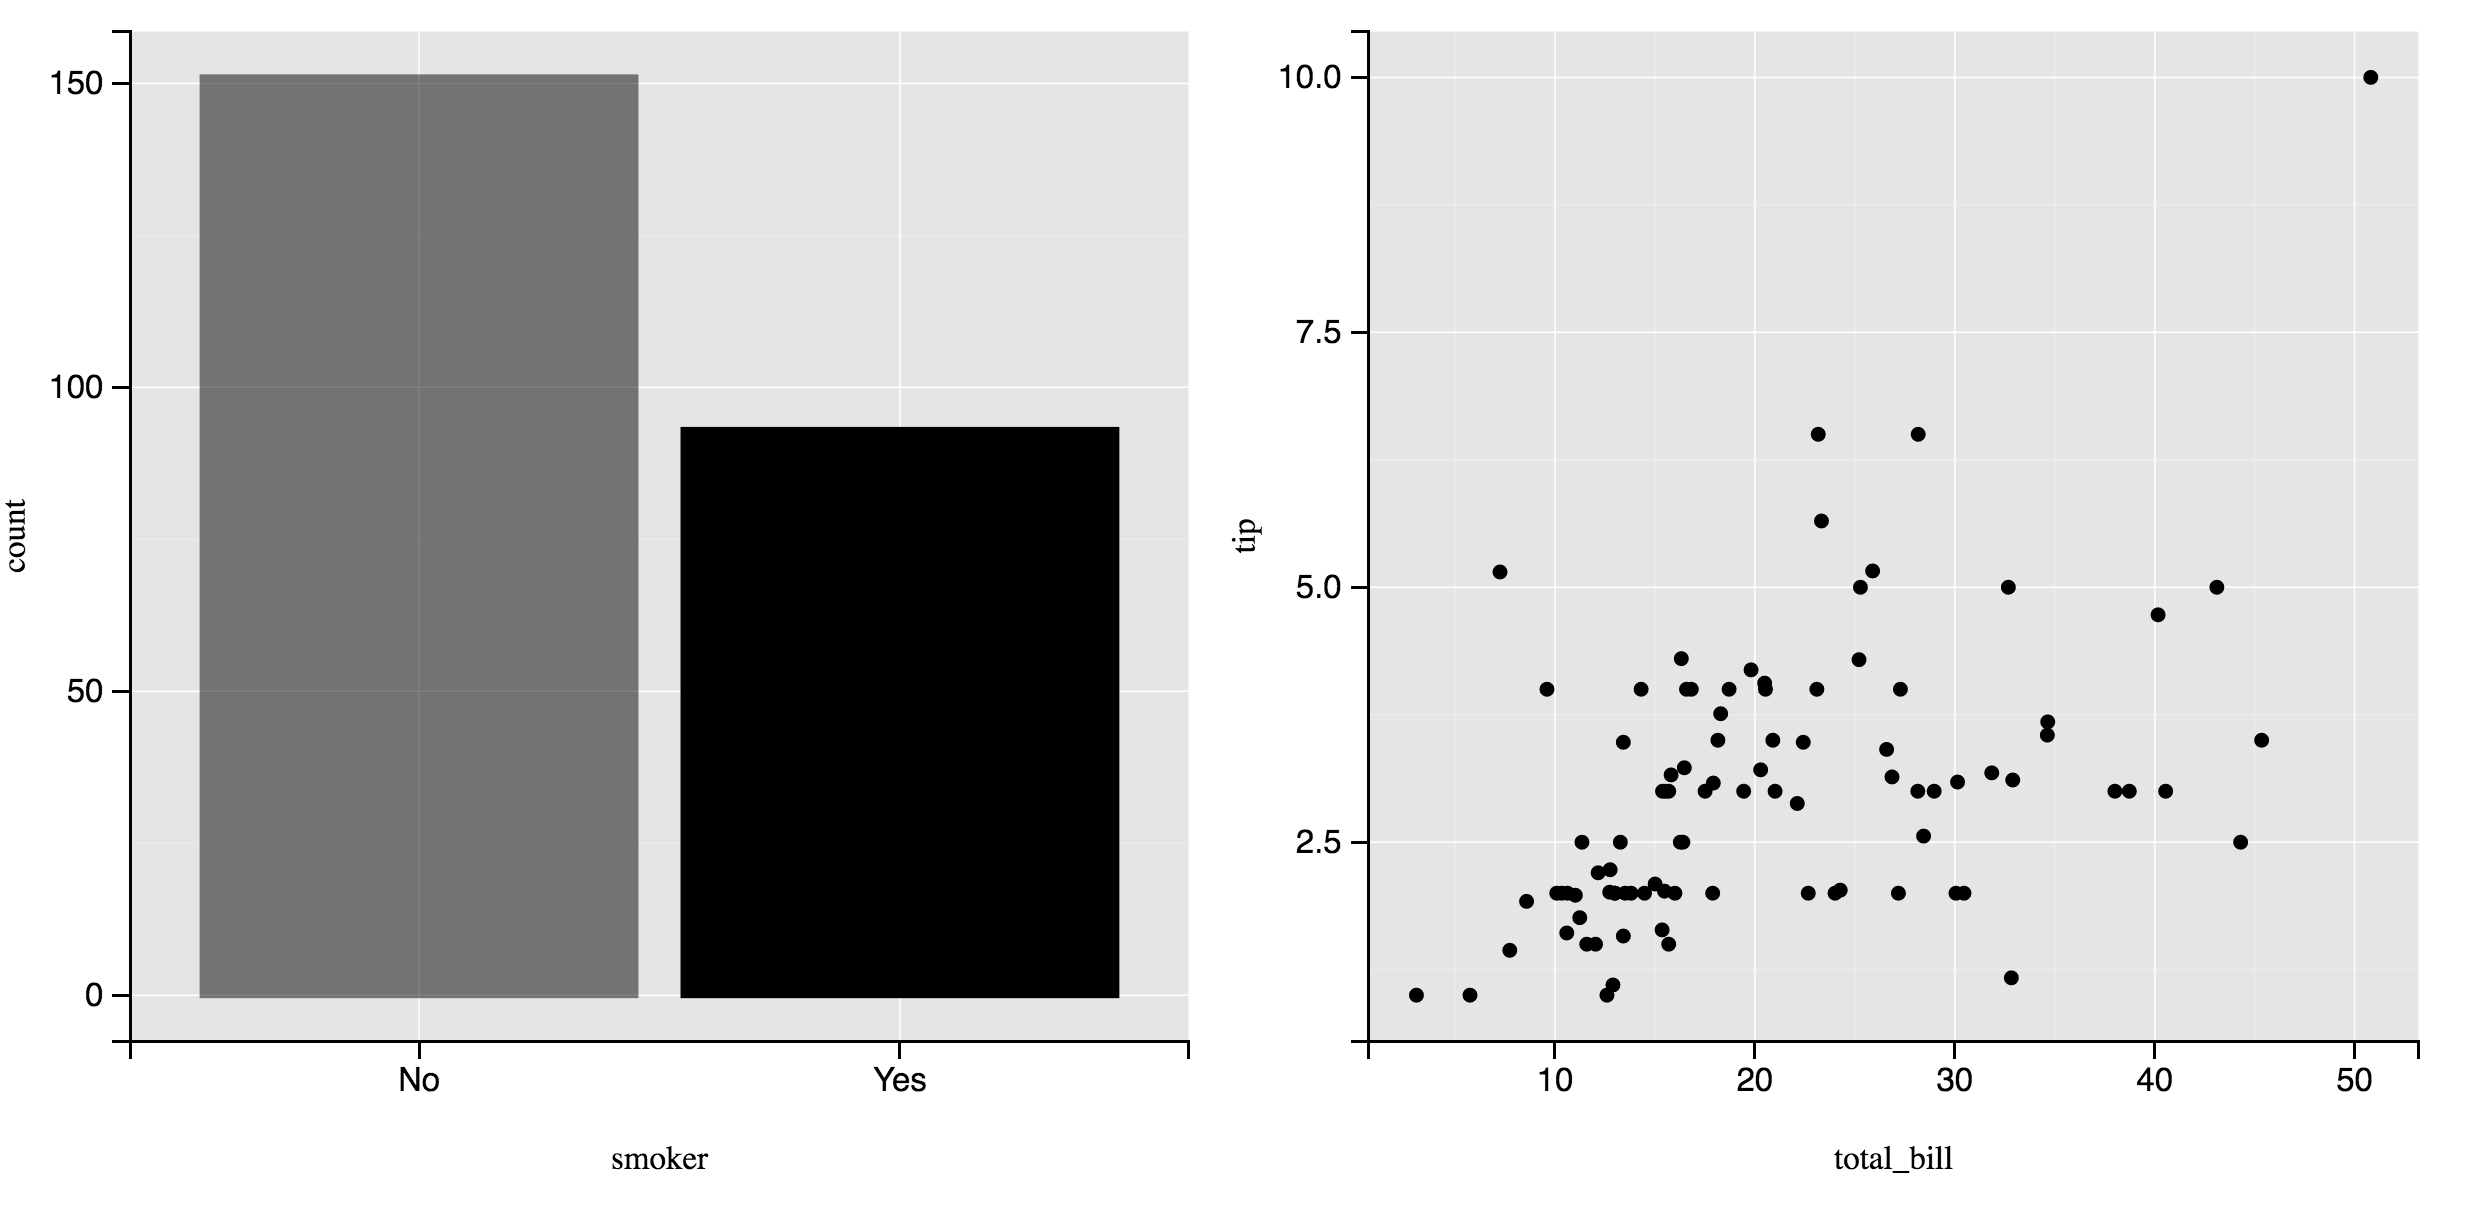
\includegraphics{images/tips}
\caption{\label{fig:tips}Linked database querying via direct manipulation
using animint. A video demonstration can be viewed online at
\url{https://vimeo.com/160496419}}
\end{figure}

In essense, the R code above allows us to use direct manipulation to
dynamically perform SQL queries of the form:

\begin{Shaded}
\begin{Highlighting}[]
\KeywordTok{SELECT} \NormalTok{total_bill, tip }\KeywordTok{FROM} \NormalTok{tips}
  \KeywordTok{WHERE} \NormalTok{smoker }\KeywordTok{IN} \NormalTok{clickSelects}
\end{Highlighting}
\end{Shaded}

In this example, \texttt{clickSelects} is either ``Yes'' or ``No'', but
as we show in later examples, \texttt{clickSelects} can also be an array
of values. Although \texttt{clickSelects} is tied to a mouseclick event,
this same framework supports other selection events, such as hover or
click+drag. Statistically speaking, this is useful for visualizing and
navigating through joint distributions conditional upon discrete values.
In this sense, our extension is closely related to the same a basis
which leads to trellis displays (Becker, Cleveland, and Shyu
\protect\hyperlink{ref-trellis}{2010}) and linked scatterplot brushing
(Becker and Cleveland
\protect\hyperlink{ref-brushing-scatterplots}{1987}). The major
differences are that conditioning: is layer (i.e., not plot) specific,
is not tied to a particular geometry, and can be controlled through
direct manipulation or animation controls. \%\% TODO: make connections
to scagnostics? trelliscope?

\subsection{Adding animation}
\label{sec:animation}

In some sense, the \texttt{showSelected} aesthetic splits the layer into
subsets -- one for every unique value of the \texttt{showSelected}
variable. The \texttt{clickSelects} aesthetics provides a mechanism to
alter the visibility of those subset(s) via direct manipulation, but our
system also provides a mechanism for automatically looping through
selections to produce animation(s). We acheive this by reserving the
name \texttt{time} to specify which variable to select as well as the
amount of time to wait before changing the selection (in milliseconds).
We also reserve the name \texttt{duration} to specify the amount of time
used to smoothly transition between frames (with linear easing). The
code below was used to generate
Figure\textasciitilde{}\ref{fig:animation} which demonstrates a simple
animation with smooth transitions between 10 frames of a single point.
Note that the resulting web page has controls for interactively altering
the \texttt{time} and \texttt{duration} parameters.

\begin{Shaded}
\begin{Highlighting}[]
\NormalTok{d <-}\StringTok{ }\KeywordTok{data.frame}\NormalTok{(}\DataTypeTok{v =} \DecValTok{1}\NormalTok{:}\DecValTok{10}\NormalTok{)}
\NormalTok{plotList <-}\StringTok{ }\KeywordTok{list}\NormalTok{(}
  \DataTypeTok{plot =} \KeywordTok{ggplot}\NormalTok{() +}\StringTok{ }\KeywordTok{geom_point}\NormalTok{(}
    \DataTypeTok{data =} \NormalTok{d, }\KeywordTok{aes}\NormalTok{(}\DataTypeTok{x=}\NormalTok{v, }\DataTypeTok{y=}\NormalTok{v, }\DataTypeTok{showSelected=}\NormalTok{v)}
  \NormalTok{),}
  \DataTypeTok{time =} \KeywordTok{list}\NormalTok{(}\DataTypeTok{variable =} \StringTok{"v"}\NormalTok{, }\DataTypeTok{ms =} \DecValTok{1000}\NormalTok{),}
  \DataTypeTok{duration =} \KeywordTok{list}\NormalTok{(}\DataTypeTok{v =} \DecValTok{1000}\NormalTok{)}
\NormalTok{)}
\KeywordTok{animint2dir}\NormalTok{(plotList)}
\end{Highlighting}
\end{Shaded}

\begin{figure}[htbp]
\centering
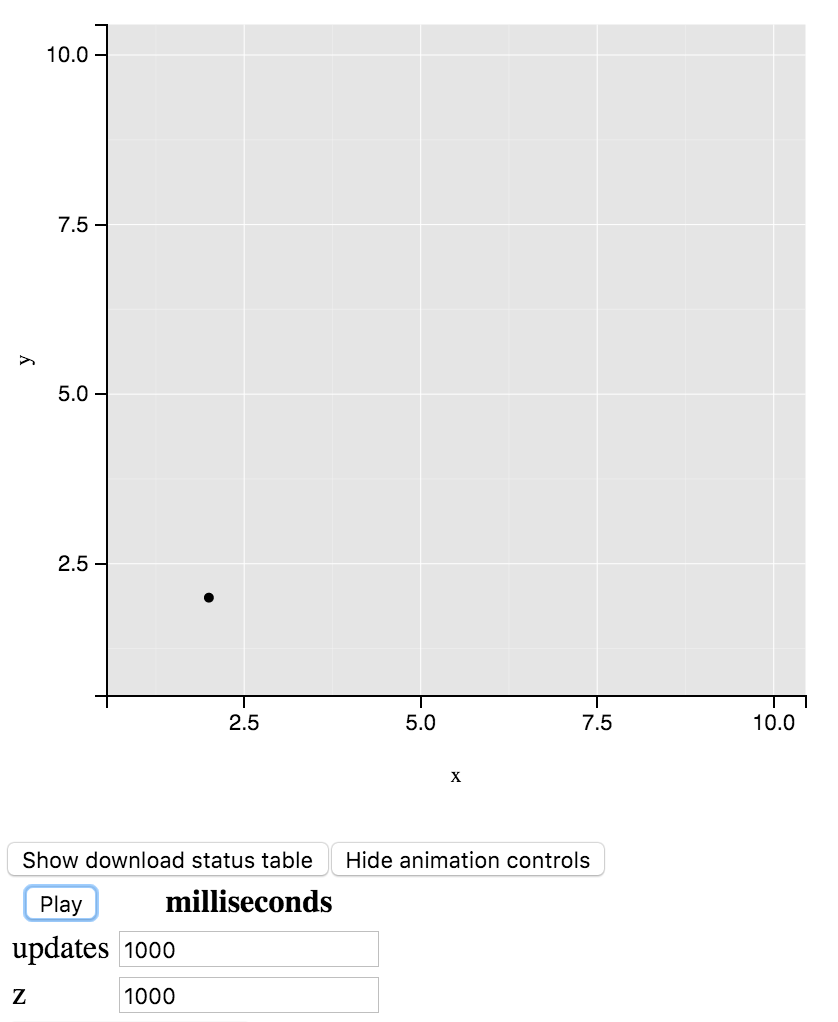
\includegraphics{images/animation}
\caption{\label{fig:animation}A simple animation with smooth transitions and
interactively altering transition durations. A video demonstration can
be viewed online at \url{https://vimeo.com/160505146}}
\end{figure}

\subsection{World Bank Example}
\label{sec:worldbank}

Figure\textasciitilde{}\ref{fig:worldbank} shows an interactive
animation of the World Bank data set (World Bank
\protect\hyperlink{ref-WorldBank}{2012}) created with our animint
implementation. The visualization helps us explore the change in the
relationship between life expectancy and fertility over time for 205
countries. By default, the year 1979 and the countries United States and
Vietnam are selected, but readers are encouraged to watch the video of
the animation and/or interact the visualization using a web
browser.\footnote{\url{http://bl.ocks.org/tdhock/raw/8ce47eebb3039263878f/}}
In the interactive version, the selected value of the year variable is
automatically incremented every few seconds, using animation to
visualize yearly changes in the relationship between life expectancy and
fertility rate.

\begin{figure}[htbp]
\centering
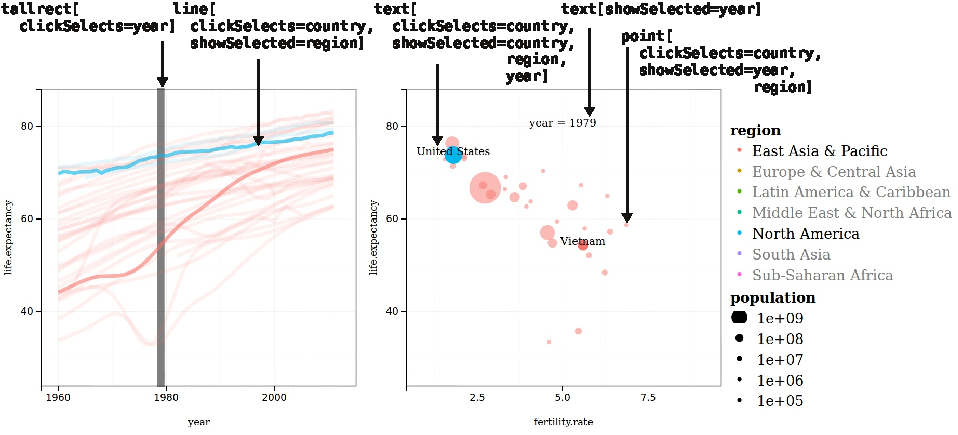
\includegraphics{images/figure-1.pdf}
\caption{\label{fig:worldbank}An interactive animation of World Bank
demographic data of several countries, designed using
\texttt{clickSelects} and \texttt{showSelected} keywords (top). Left: a
multiple time series from 1960 to 2010 of life expectancy, with bold
lines showing the selected countries and a vertical grey tallrect
showing the selected year. Right: a scatterplot of life expectancy
versus fertility rate of all countries. The legend and text elements
show the current selection: year=1979, country= \{United States,
Vietnam\}, and region=\{East Asia \& Pacific, North America\}}
\end{figure}

When viewing the interactive version of
Figure\textasciitilde{}\ref{fig:worldbank}, suppose we wish to select
Thailand. Direct manipulation is not very useful in this case since it
is not easy to identify and select Thailand based on graphical marks on
a plot. For this reason, animint also provides dropdown menu(s) for each
selection variable to aid the selection process.
Figure\textasciitilde{}\ref{fig:widgets} shows what the user sees after
typing ``th'' in the search box. Note that these dropdowns support
selection of multiple values and coordinate sensibly with selections
made via direct manipulation.

\begin{figure}[htbp]
\centering
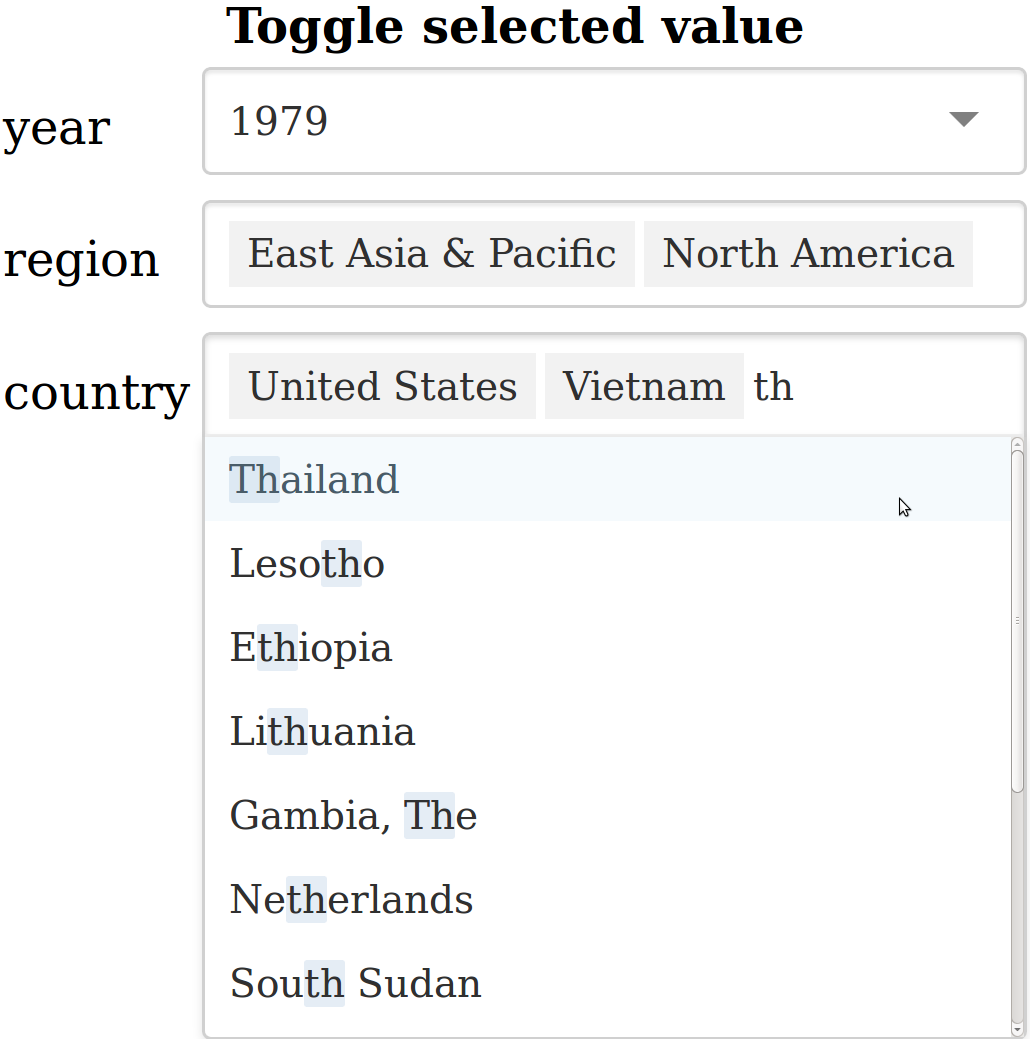
\includegraphics{images/Screenshot-toggle-selected-value}
\caption{\label{fig:widgets}Animint provides a menu to update each selection
variable. In this example, after typing `th' the country menu shows the
subset of matching countries.}
\end{figure}

We anticipate that some ggplot2 users will be able to reverse engineer
the animint code which creates
Figure\textasciitilde{}\ref{fig:worldbank}, simply by looking at it. In
fact, this is a big reason why ggplot2 is so widely used: it helps
minimize the amount of time required to translate a figure that exists
in your head into computer code. Note that, in the left hand plot of
Figure\textasciitilde{}\ref{fig:worldbank}, we have a time series of the
life expectancy where each line is a country (i.e., we \texttt{group} by
country) and lines are colored by region. By clicking on a line, we also
want the country label to appear in the right hand plot, so we also need
to set \texttt{clickSelects=country}. Lastly, by setting
\text{showSelected=region}, we can hide/show lines by clicking on the
color legend entries.

\begin{Shaded}
\begin{Highlighting}[]
\NormalTok{timeSeries <-}\StringTok{ }\KeywordTok{ggplot}\NormalTok{() +}\StringTok{ }\KeywordTok{geom_line}\NormalTok{(}
  \DataTypeTok{data =} \NormalTok{WorldBank,}
  \KeywordTok{aes}\NormalTok{(}\DataTypeTok{x =} \NormalTok{year, }\DataTypeTok{y =} \NormalTok{life.expectancy,}
      \DataTypeTok{group =} \NormalTok{country, }\DataTypeTok{color =} \NormalTok{region,}
      \DataTypeTok{clickSelects =} \NormalTok{country, }
      \DataTypeTok{showSelected =} \NormalTok{region)}
\NormalTok{)}
\end{Highlighting}
\end{Shaded}

We want to provide a visual clue for the selected year in the time
series, so we also layer some ``tall rectangles" onto the time series.
These tall rectangles will also serve as a way to directly modify the
selected year. The tallrect geometry is a special case of a rectangle
that automatically spans the entire vertical range, so we just have to
specify the horizontal range via \texttt{xmin} and \texttt{xmax}. Also,
since the layered grammar of graphics allows for different data in each
layer, we supply a data frame with just the unique years in the entire
data for this layer.

\begin{Shaded}
\begin{Highlighting}[]
\NormalTok{years <-}\StringTok{ }\KeywordTok{data.frame}\NormalTok{(}\DataTypeTok{year =} \KeywordTok{unique}\NormalTok{(WorldBank$year))}
\NormalTok{timeSeries <-}\StringTok{ }\NormalTok{timeSeries +}\StringTok{ }\KeywordTok{geom_tallrect}\NormalTok{(}
  \DataTypeTok{data =} \NormalTok{years,}
  \KeywordTok{aes}\NormalTok{(}\DataTypeTok{xmin =} \NormalTok{year -}\StringTok{ }\FloatTok{0.5}\NormalTok{, }\DataTypeTok{xmax =} \NormalTok{year +}\StringTok{ }\FloatTok{0.5}\NormalTok{,}
      \DataTypeTok{clickSelects =} \NormalTok{year)}
\NormalTok{)}
\end{Highlighting}
\end{Shaded}

As for the right hand plot in
Figure\textasciitilde{}\ref{fig:worldbank}, there are three layers: a
point layer for countries, a text layer for countries, and a text layer
to display the selected year. By clicking on a point, we want to display
the country text label and highlight the corresponding time series on
the right hand plot, so we set \texttt{clickSelects=country} in this
layer. Furthermore, we only want to show the points for the selected
year and region, so we also need \texttt{showSelected=year} and
\texttt{showSelected2=region}.

\begin{Shaded}
\begin{Highlighting}[]
\NormalTok{scatterPlot <-}\StringTok{ }\KeywordTok{ggplot}\NormalTok{() +}\StringTok{ }\KeywordTok{geom_point}\NormalTok{(}
  \DataTypeTok{data =} \NormalTok{WorldBank,}
  \KeywordTok{aes}\NormalTok{(}\DataTypeTok{x =} \NormalTok{fertility.rate, }\DataTypeTok{y =} \NormalTok{life.expectancy,}
      \DataTypeTok{color =} \NormalTok{region, }\DataTypeTok{size =} \NormalTok{population,}
      \DataTypeTok{clickSelects =} \NormalTok{country,}
      \DataTypeTok{showSelected =} \NormalTok{year,}
      \DataTypeTok{showSelected2 =} \NormalTok{region)}
\NormalTok{)}
\end{Highlighting}
\end{Shaded}

The text layer for annotating selected countries is essentially the same
as the point layer, except we map the country name to the \texttt{label}
aesthetic.

\begin{Shaded}
\begin{Highlighting}[]
\NormalTok{scatterPlot <-}\StringTok{ }\NormalTok{scatterPlot +}\StringTok{ }\KeywordTok{geom_text}\NormalTok{(}
  \DataTypeTok{data =} \NormalTok{WorldBank,}
  \KeywordTok{aes}\NormalTok{(}\DataTypeTok{x =} \NormalTok{fertility.rate, }\DataTypeTok{y =} \NormalTok{life.expectancy,}
      \DataTypeTok{label =} \NormalTok{country,}
      \DataTypeTok{showSelected =} \NormalTok{country,}
      \DataTypeTok{showSelected2 =} \NormalTok{year,}
      \DataTypeTok{showSelected3 =} \NormalTok{region)}
\NormalTok{)}
\end{Highlighting}
\end{Shaded}

Lastly, to help identify the selected year when viewing the scatterplot,
we add another layer of text at a fixed location.

\begin{Shaded}
\begin{Highlighting}[]
\NormalTok{scatterPlot <-}\StringTok{ }\NormalTok{scatterPlot +}\StringTok{ }\KeywordTok{geom_text}\NormalTok{(}
  \DataTypeTok{data =} \NormalTok{years, }\DataTypeTok{x =} \DecValTok{5}\NormalTok{, }\DataTypeTok{y =} \DecValTok{80}\NormalTok{,}
  \KeywordTok{aes}\NormalTok{(}\DataTypeTok{label =} \KeywordTok{paste}\NormalTok{(}\StringTok{"year ="}\NormalTok{, year),}
      \DataTypeTok{showSelected =} \NormalTok{year)}
\NormalTok{)}
\end{Highlighting}
\end{Shaded}

Now that we have defined the plots in
Figure\textasciitilde{}\ref{fig:worldbank}, we can set the \texttt{time}
and \texttt{duration} options (introduced in
Section\textasciitilde{}\ref{sec:animation}) to control the animation
parameters. Our animint implementation also respects a
\texttt{selector.types} option which controls whether or not selections
for a given variable can accumulate and a \texttt{first} option for
controlling which values are selected by default.
\footnote{We maintain a complete list of (animint specific) options here --
\url{https://github.com/tdhock/animint/wiki/Advanced-features-present-animint-but-not-in-ggplot2}}
By default, supplying the list of plots and additional options to
\texttt{animint2dir()} will write all the files necessary to render the
visualization to a temporary directory and prompt a web browser to open
an HTML file.

\begin{Shaded}
\begin{Highlighting}[]
\NormalTok{viz <-}\StringTok{ }\KeywordTok{list}\NormalTok{(}
  \DataTypeTok{timeSeries =} \NormalTok{timeSeries,}
  \DataTypeTok{scatterPlot =} \NormalTok{scatterPlot,}
  \DataTypeTok{time =} \KeywordTok{list}\NormalTok{(}\DataTypeTok{variable =} \StringTok{"year"}\NormalTok{, }\DataTypeTok{ms =} \DecValTok{3000}\NormalTok{),}
  \DataTypeTok{duration =} \KeywordTok{list}\NormalTok{(}\DataTypeTok{year =} \DecValTok{1000}\NormalTok{),}
  \DataTypeTok{selector.types =} \KeywordTok{list}\NormalTok{(}
    \DataTypeTok{year =} \StringTok{"single"}\NormalTok{,}
    \DataTypeTok{country =} \StringTok{"multiple"}\NormalTok{,}
    \DataTypeTok{region =} \StringTok{"multiple"}
  \NormalTok{),}
  \DataTypeTok{first =} \KeywordTok{list}\NormalTok{(}
    \DataTypeTok{country =} \KeywordTok{c}\NormalTok{(}\StringTok{"United States"}\NormalTok{, }\StringTok{"Thailand"}\NormalTok{)}
  \NormalTok{)}
\NormalTok{)}
\KeywordTok{animint2dir}\NormalTok{(viz)}
\end{Highlighting}
\end{Shaded}

\subsection{Implementation details}
\label{sec:implementation}

As shown in Figure\textasciitilde{}\ref{fig:design}, the animint system
is implemented in 2 parts: the compiler and the renderer. The compiler
is implemented in about 2000 lines of R code that converts a list of
ggplots and options to a JSON plot meta-data file and a tab-separated
values (TSV) file database.

\begin{figure}[htbp]
\centering
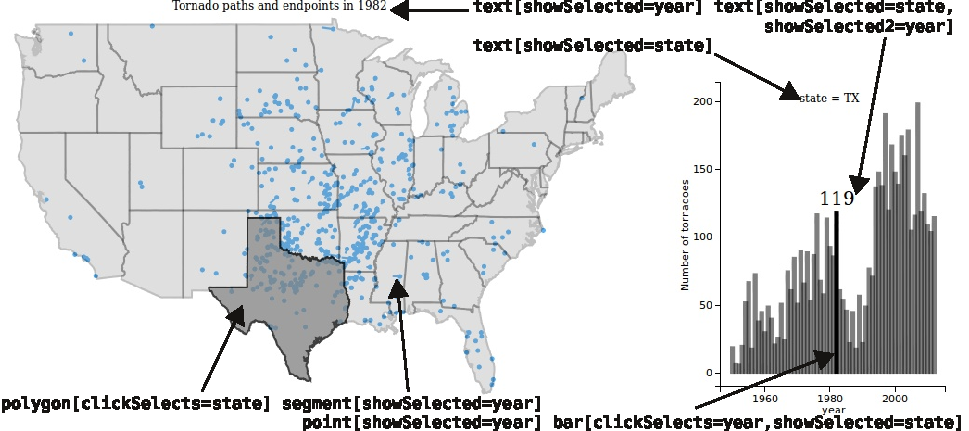
\includegraphics{images/figure-tornado.pdf}
\caption{\label{fig:tornado}Interactive animation of tornadoes recorded from
1950 to 2012 in the United States. Left: map of the lower 48 United
States with tornado paths in 1982. The text shows the selected year, and
clicking the map changes the selected state, currently Texas. Right:
time series of tornado counts in Texas. Clicking a bar changes the
selected year, and the text shows selected state and the number of
tornadoes recorded there in that year (119 tornadoes in Texas in 1982).}
\end{figure}

\begin{figure}[htbp]
\centering
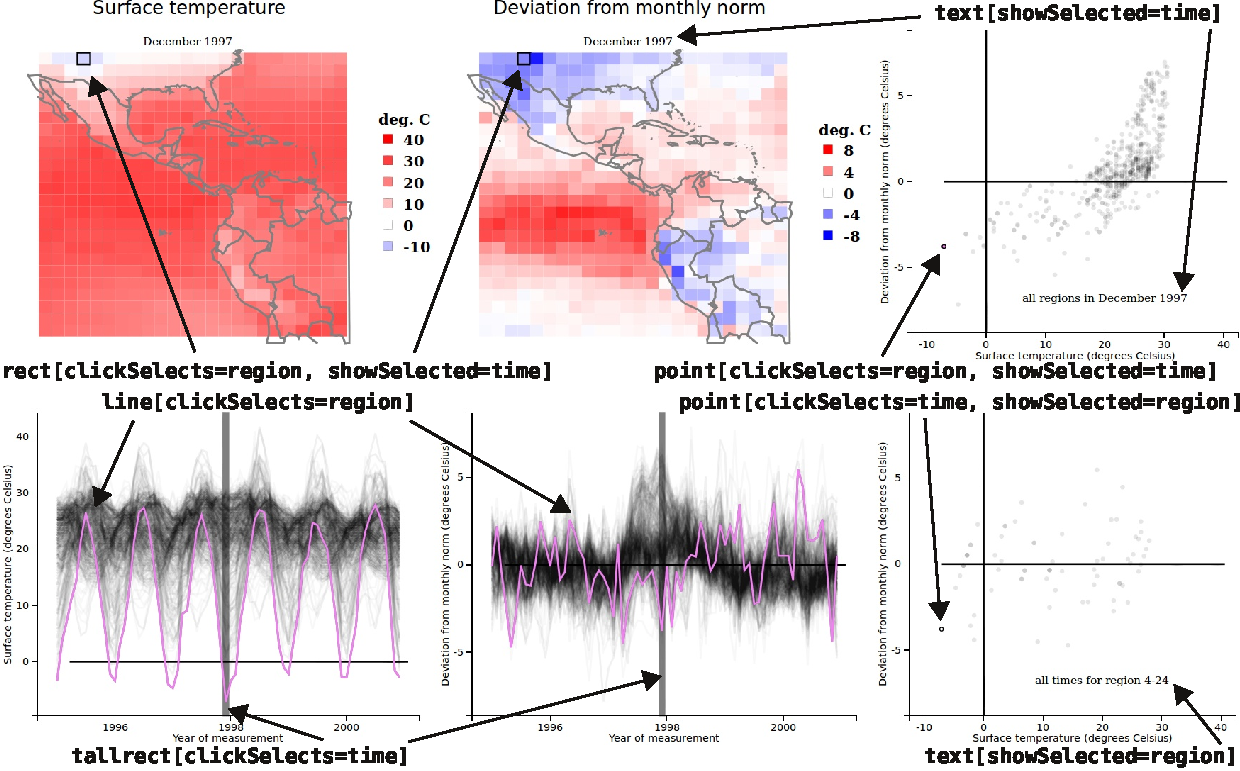
\includegraphics{images/figure-climate.pdf}
\caption{\label{fig:climate}Visualization containing 6 linked, interactive,
animated plots of Central American climate data. Top: for the selected
time (December 1997), maps displaying the spatial distribution of two
temperature variables, and a scatterplot of these two variables. The
selected region is displayed with a black outline, and can be changed by
clicking a rect on the map or a point on the scatterplot. Bottom: time
series of the two temperature variables with the selected region shown
in violet, and a scatterplot of all times for that region. The selected
time can be changed by clicking a background tallrect on a time series
or a point on the scatterplot. The selected region can be changed by
clicking a line on a time series.}
\end{figure}

The compiler scans the aesthetics in the ggplots to determine how many
selection variables are present, and which geoms to update after a
selection variable is updated. It uses ggplot2 to automatically
calculate the axes scales, legends, labels, backgrounds, and borders. It
outputs this information to the JSON plot meta-data file.

The compiler also uses ggplot2 to convert data variables (e.g.~life
expectancy and region) to visual properties (e.g.~y position and color).
The data for each layer/geom are saved in several TSV files, one for
each combination showSelected values. Thus for large data sets, the web
browser only needs to download the subset of data required to render the
current selection (Heer \protect\hyperlink{ref-2013-immens}{2013}).

When repeated data would be saved in each of the TSV files, an extra
common TSV file is created so that the repeated data only need to be
stored and downloaded once. In that case, the other TSV files do not
store the common data, but are merged with the common data after
downloading. This method for constructing the TSV file database was
developed to minimize the disk usage of animint, particularly for
ggplots of spatial maps as in Figure\textasciitilde{}\ref{fig:tornado}.

Finally, the rendering engine (\texttt{index.html}, \texttt{d3.v3.js},
and \texttt{animint.js} files) is copied to the plot directory. The
\texttt{animint.js} renderer is implemented in about 2200 lines of
JavaScript/D3 code that renders the TSV and JSON data files as SVG in a
web browser. Importantly, animation is achieved by using the JavaScript
\texttt{setInterval} function, which updates the \texttt{time} selection
variable every few seconds. Since the compiled plot is just a directory
of files, the interactive plots can be hosted on any web server. The
interactive plots can be viewed by opening the \texttt{index.html} page
in any modern web browser.

\section{Exploring performance \& scope with examples}
\label{sec:performance}

This section attempts to demonstrate a range of visualizations that are
supported by animint with more examples.
Figure\textasciitilde{}\ref{fig:tornado} shows an interactive animation
of tornadoes observed in the United States between 1950 and 2012. At any
moment in time, the user can simultaneously view the spatial
distribution of tornadoes in the selected year over all states, and see
the trend over all years for the selected state. Clicking a state on the
map updates the time series bars to show the tornado counts from that
state. Clicking a bar on the time series updates the selected year.
Figure\textasciitilde{}\ref{fig:climate} shows an interactive animation
of climate time series data observed in Central America. Two maps
display the spatial distribution of two temperature variables, which are
shown over time in corresponding the time series plots below.
Scatterplots also show the relationships between the two temperature
variables for the selected time and region. Clicking any of the plots
updates all 6 of them. The \texttt{clickSelects} and
\texttt{showSelected} aesthetics make it easy to design this set of 6
linked plots in only 87 lines of code.

Summary statistics describing complexity and performance for examples in
this paper, as well as other animint examples, are displayed in
Table\textasciitilde{}\ref{tab:examples}. The climate data visualization
has noticeably slow animations, since it displays about 88,980 geometric
elements at once (\url{http://bit.ly/QcUrhn}). We observed this slowdown
across all browsers, which suggested that there is an inherent
bottleneck when rendering large interactive plots in web browsers using
JavaScript and SVG. Another animint with a similar amount of total rows
is based on the evolution data (\url{http://bit.ly/O0VTS4}), but since
it shows less data onscreen (about 2703 elements), it exhibits faster
responses to interactivity and animation.

Animint is still useful for creating interactive but non-animated plots
when there is not a time variable in the data. In fact, 7 of the 11
examples in Table\textasciitilde{}\ref{tab:examples} are not animated.
For example, linked plots are useful to illustrate complex concepts such
as a change point detection model in the breakpoints data
(\url{http://bit.ly/1gGYFIV}). The user can explore different model
parameters and data sets since these are encoded as animint interaction
variables.

\begin{table*}[htp] % This table is too wide to fill in the page.
  \centering
  % latex table generated in R 3.1.1 by xtable 1.7-3 package
% Thu Oct  9 14:20:02 2014
\begin{tabular}{rrrrrrrrrrr}
  \hline
 & LOC & seconds & MB & rows & onscreen & variables & interactive & plots & animated? & Fig \\ 
  \hline
worldPop & 17 & 0.2 & 0.1 & 924 & 624 &  4 &  2 &  2 & yes &  \\ 
  WorldBank & 20 & 2.3 & 2.1 & 34132 & 11611 &  6 &  2 &  2 & yes &  \ref{fig:worldbank} \\ 
  evolution & 25 & 21.6 & 12.0 & 240600 & 2703 &  5 &  2 &  2 & yes &  \\ 
  change & 36 & 2.8 & 2.5 & 36238 & 25607 & 12 &  2 &  3 & no &  \\ 
  tornado & 39 & 1.7 & 6.1 & 103691 & 16642 & 11 &  2 &  2 & no &  \ref{fig:tornado} \\ 
  prior & 54 & 0.7 & 0.2 & 1960 & 142 & 12 &  3 &  4 & no &  \\ 
  compare & 66 & 10.7 & 7.9 & 133958 & 2140 & 20 &  2 &  5 & no &  \\ 
  breakpoints & 68 & 0.5 & 0.3 & 4242 & 667 & 13 &  2 &  3 & no &  \\ 
  climate & 84 & 12.8 & 19.7 & 253856 & 88980 & 15 &  2 &  6 & yes &  \ref{fig:climate} \\ 
  scaffolds & 110 & 56.3 & 78.5 & 618740 & 9051 & 30 &  3 &  3 & no &  \\ 
  ChIPseq & 229 & 29.9 & 78.3 & 1292464 & 1156 & 44 &  4 &  5 & no & \\ 
   \hline
\end{tabular}

  \vskip 0.2cm
  \caption{Characteristics of 11 interactive visualizations designed with
    animint. The interactive version of these visualizations can be accessed 
    via \url{http://sugiyama-www.cs.titech.ac.jp/~toby/animint/}.
    From left to right, we show the data set name, the
    lines of R code (LOC) including data processing but not including comments
    (80 characters max per line),
    the amount of time it takes to compile the visualization (seconds),
    the total size of the uncompressed TSV files in megabytes (MB),
    the total number of data points (rows),
    the median number of data points shown at once (onscreen),
    the number of data columns visualized (variables),
    the number of \texttt{clickSelects}/\texttt{showSelected} 
    variables (interactive),
    the number of linked panels (plots),
    if the plot is animated,
    and the corresponding Figure number in this paper (Fig).
  }
\label{tab:examples}
\end{table*}

\section{Comparison study}
\label{sec:compare}

In this section we compare our animint implementation with other similar
leading systems by creating a given visualization in each system and
discussing the pros and cons of the different approaches.

\subsection{The Grand Tour}
\label{sec:tour}

The Grand Tour is a well-known method for viewing high dimensional data
which requires interactive and dynamic graphics (Asimov
\protect\hyperlink{ref-grand-tour}{1985}).
Figure\textasciitilde{}\ref{fig:tour} shows a grand tour of 300
observations sampled from a correlated tri-variate normal distribution.
The left hand view shows the marginal density of each point while the
right hand view ``tours" through 2D projections of the 3D data. There
are many ways to choose projections in a tour, and many ways to
interpolate between projections, most of which can be programmed fairly
easily using R and relevant add-on packages. In this case, we used the R
package tourr, which uses the geodesic random walk (i.e., random 2D
projection with geodesic interpolation) in its grand tour algorithm
(Wickham et al. \protect\hyperlink{ref-tourr}{2011}).

\begin{figure}[htbp]
\centering
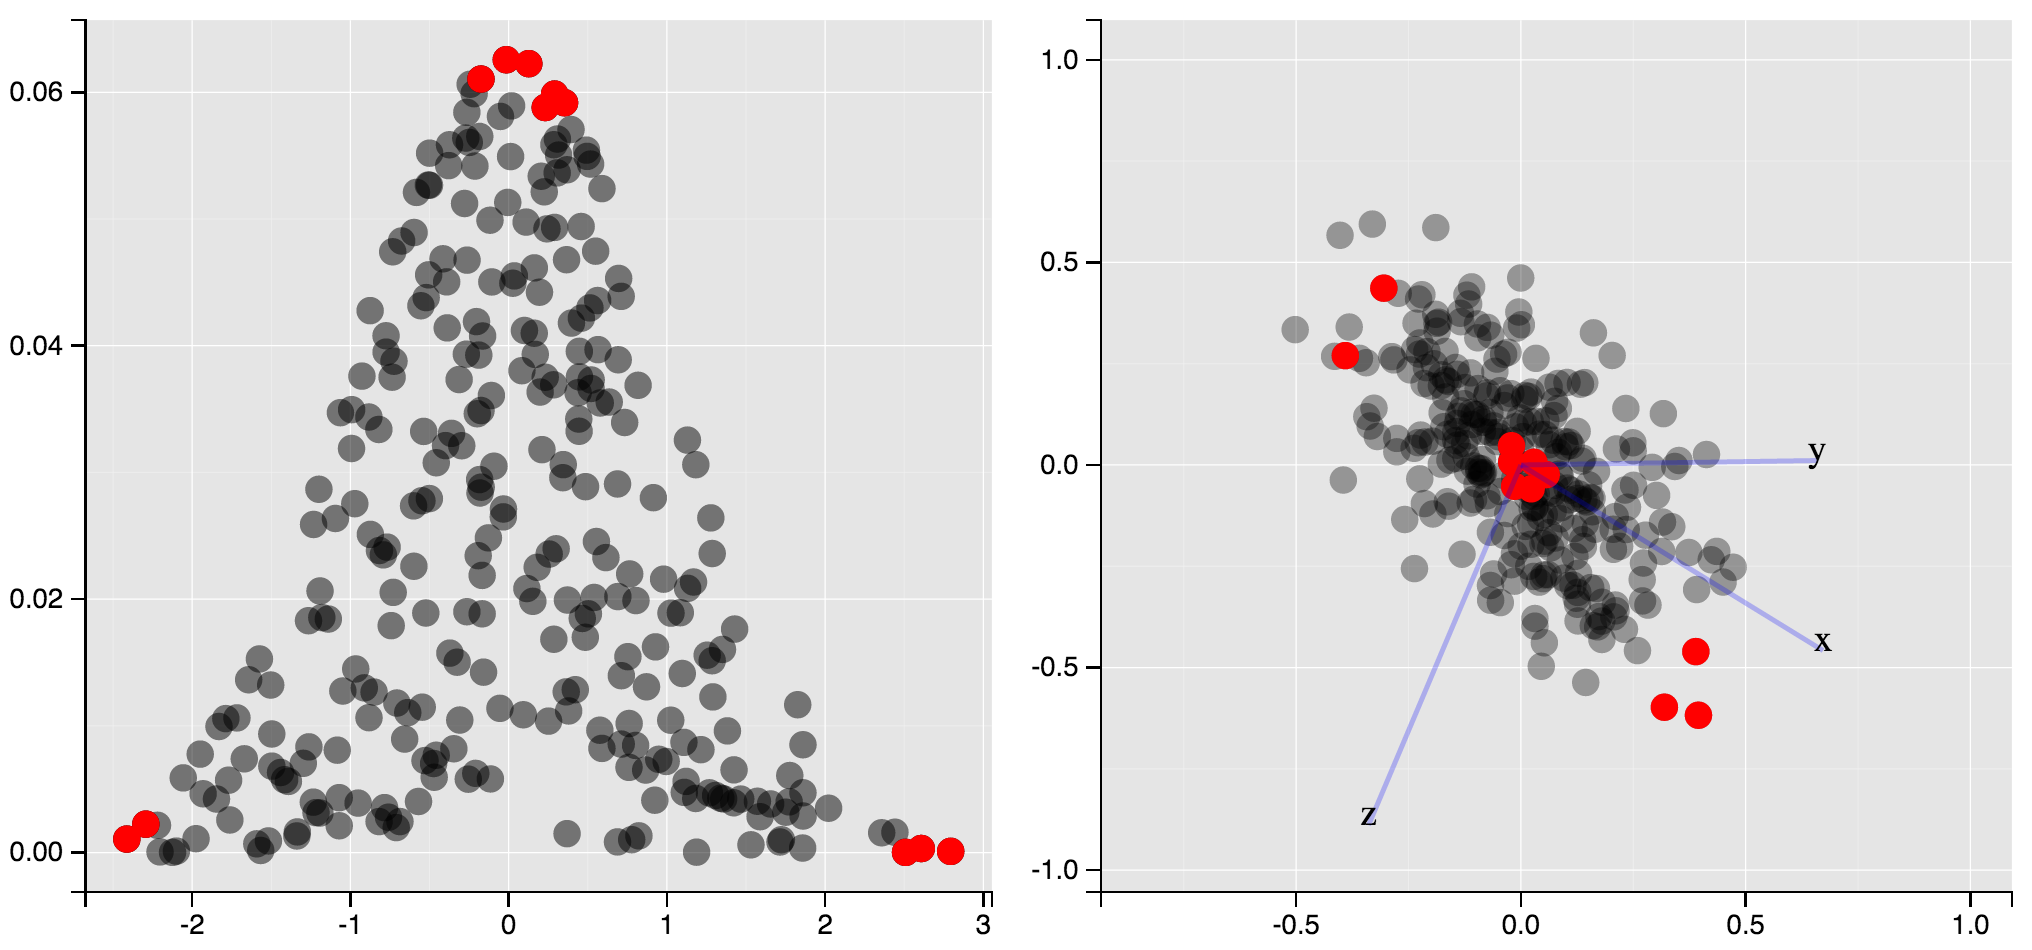
\includegraphics{images/tour}
\caption{\label{fig:tour}Linked selection in a grand tour with animint. A
video demonstration can be viewed online at
\url{https://vimeo.com/160720834}}
\end{figure}

When touring data, it is generally useful to link low-dimensional
displays with the tour itself. The video in
Figure\textasciitilde{}\ref{fig:tour} was generated with our current
animint implementation, and points are selected via mouse click which
reveal that points with high marginal density are located in the
ellipsoid center while points with a low marginal density appear near
the ellipsoid border. In this case, it would be convenient to also have
brush selection, as we demonstrate in
Figure\textasciitilde{}\ref{fig:tourbrush} which implements the same
touring example using the R packages ggvis and shiny. The brush in
Figure\textasciitilde{}\ref{fig:tourbrush} is implemented with shiny's
support for brushing static images, which currently does not support
multiple brushes, making it difficult to select non-contiguous regions.

\begin{figure}[htbp]
\centering
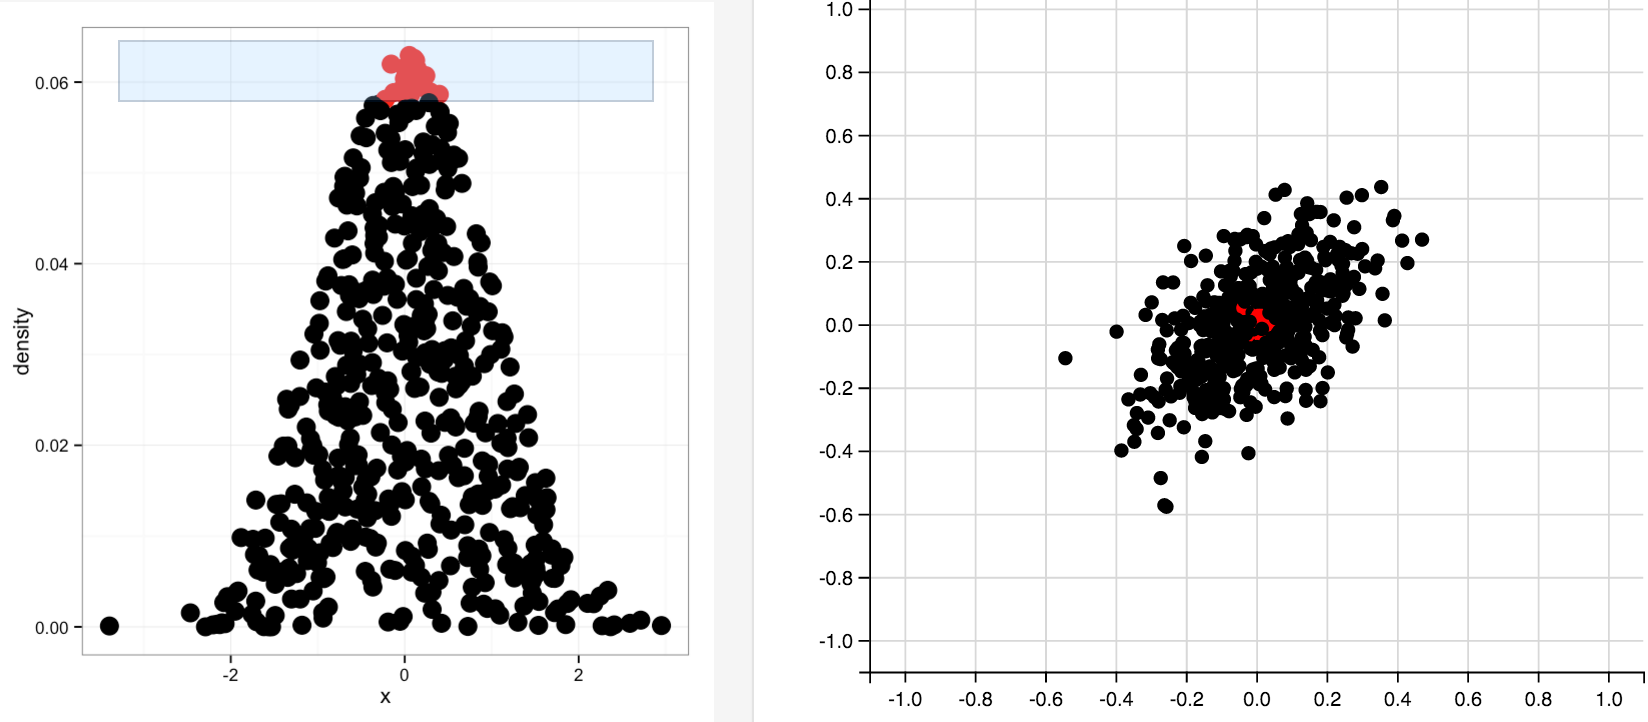
\includegraphics{images/tourbrush}
\caption{\label{fig:tourbrush}Linked selection in a grand tour with ggvis
and shiny. A video demonstration can be viewed online at
\url{https://vimeo.com/160825528}}
\end{figure}

This example helps point out a few other important differences in using
animint versus ggvis+shiny to implement ``multiple linked and dynamic
views" as described in (Ahlberg, Williamson, and Shneiderman
\protect\hyperlink{ref-Ahlberg:1991}{1991}) and (Buja et al.
\protect\hyperlink{ref-Buja:1991vh}{1991}). Maintaining state of the
linked brush in Figure\textasciitilde{}\ref{fig:tourbrush} requires both
knowledge and clever use of some sophicated programming techniques such
as closures and reactivity. It also requires knowledge of the shiny web
application framework and a new approach to the grammar of graphics. On
the other hand, maintaining state in
Figure\textasciitilde{}\ref{fig:tour} requires a few different
\texttt{clickSelects}/\texttt{showSelected} mappings. As a result, we
believe animint provides a more elegant user interface for this
application.

The tourring example also helps point out important consequences of the
design and implementation of these two different systems. As mentioned
in Section\textasciitilde{}\ref{sec:implementation}, our current animint
implementation requires every subset of data to be precomputed before
render time. For visualizations such as tours, where it is more
efficient to perform statistical computations on-the-fly, this can be a
harsh restriction, but this is a restriction of our current
implementation (not a restriction of the framework itself). As a result,
when touring a large high-dimensional space, where many projections are
needed, ggvis+shiny may be desirable since the projections are computed
on the server and sent to the browser in real-time. This works fine when
the application is running and viewed on the same host machine, but
viewing such an application hosted on a remote machine can produce
staggered animations since client-server requests must be performed,
processed, and rendered roughly 30 times a second. Also, generally
speaking, the animint system results a more pleasant experience when it
comes to hosting and sharing applications since it doesn't require a Web
Server with R and special software already installed.

\subsection{World Bank Example}

We also recreated Figure\textasciitilde{}\ref{fig:worldbank} using
ggvis+shiny (see \url{http://bit.ly/1SsJKlN}) and Tableau (see
\url{http://bit.ly/worldBank-tableau}). Even as experienced ggvis+shiny
users, we found it quite difficult to replicate this example, and were
not able completely replicate it due to a lack of a mechanism for
coordinating indirect and direct manipulations. Overall the
visualization is pretty similar, but lacks a few important features. In
particular, there is no way to control the selected year using both the
slider (indirect) and clicking on the ggvis plot (direct). It also lacks
the ability to click on a countries time series and label the
corresponding point on the scatterplot. This might be possible, but we
could not find a way to update a plot based on a click event on a
different plot. Even with this lack of functionality, the ggvis+shiny is
significantly more complicated and requires more code (about 100 lines
of code compared to 30).

It was also impossible to completely replicate
Figure\textasciitilde{}\ref{fig:worldbank} using Tableau essentially
because the example requires a \emph{layered} approach to the grammar of
graphics. In particular, since graphical marks and interaction
source/target(s) must derive from the same table in Tableau, it was
impossible to control the clickable multiple time series and the
clickable tallrects in different ways based on the two different
selection variables. In other words, in Tableau, selections are managed
on the plot level, but in animint, selections are specific to each
graphical layer.

\section{User feedback and observations}

By working with researchers in several fields of research, we have
created a wide variety of interactive visualizations using animint.
Typically, the researchers have a complex data set that they wish to
visualize, but they do not have the expertise or time to create an
interactive data visualization. The animint system made it easy to
collaborate with the various domain experts, who were able to provide us
with annotated sketches of the desired plots, which we then translated
to animint R code. In this section we share comments and constructive
criticism that we have obtained from our users.

\subsection{User perspective}

For the \texttt{prior} data visualization (\url{http://bit.ly/1peIT7t}),
the animint user is a machine learning researcher who developed an
algorithm and applied it to 4 benchmark data sets. He wanted to explore
how his algorithm performed, in comparison to a baseline learning
algorithm. He appreciated the intuition about his algorithm's
performance that he learned from the interactive plots: ``Interactive
plotting allows us to explore all relationships of our high-dimensional
dataset and gives us an intuitive understanding of the performance of
our proposed algorithm. An intuitive understanding of the results is
important since it shows under which conditions our proposed method
works well and provides avenues for further research.''

Another user from a machine learning background found the interactive
plots useful for presenting his work: `\texttt{the}regularization path'
is a difficult concept to demonstrate in my research. The animint
(\url{http://bit.ly/1gVb8To}) helped greatly by rendering an interactive
plot of regularization path, likelihood, and graph at the same time and
illustrating their connections. It also reveals an interesting
phenomenon that maximizing the testing likelihood actually gives many
false positives.''

In another application, the animint user was a genomics researcher:
``viewing and exploring my complex intestinal microbiome dataset in
animint allowed me to grasp the patterns and relationships between
samples at an almost intuitive level. The interactive aspect of it was
very helpful for browsing through the dataset.''

Finally, users also appreciated the simple web interface, and the detail
that is possible to show in interactive plots, but impossible to show in
publications: ``\ldots{} the web interface is simple and easy to use. It
also enables us to publish more detailed interactive results on our
website to accompany the results presented in publications.''

\subsection{Developer perspective}

R users, and in particular ggplot2 users, have found that animint is
easy to learn and use. One statistics Ph.D.~student writes, ``animint is
a fantastic framework for creating interactive graphics for someone
familiar with R and ggplot2's grammar of graphics implementation. The
API is very intuitive and allows one to quickly bring their static
graphics to life in a way that facilitates exploratory data analysis.''

\section{Limitations and future work}
\label{sec:limitations}

A number of limitations derive from the fact that some plot features are
computed once during the compilation step and remain static on a
rendered plot. For example, users are unable to change variable mappings
after compilation. Also, when different data subsets have very different
ranges of values, it may be preferable to recompute scales when
\texttt{clickSelects} selection(s) change. A future implementation of
animint would benefit from changes to the compiler and renderer that
allow scales to be updated after each click. Some of these limitations
can be resolved by adding interactive widgets to ``recompile" components
hard-coded in the plot meta information. In fact, animint makes it easy
to embed visualizations inside of shiny web applications, and we have an
example of interactively redefining variable mappings
(\url{http://bit.ly/animint-shiny}).

Our compiler also currently takes advantage of ggplot2 internals to
compute statistics and positional adjustments before rendering. As a
result, statistics/positions will not dynamically recompute based on
selections. In other words, using
\texttt{clickSelects}/\texttt{showSelected} with non-identity
statistic(s)/position(s) may not generate a sensible result. It would be
possible, but a significant amount of work, to transfer these
computations from the compiler to the renderer.

Another set of limitations derive our current restriction that all
subsets (corresponding to each possible selection) must be precomputed
before render time. As eluded to in
Section\textasciitilde{}\ref{sec:tour}, if there is a large space of
possible selections, it is impractical to precompute every subset before
viewing. Therefore, it would be useful if the renderer could dynamically
compute subsets when new selections are made.

Our implementation is also limited to two specific types of direct
manipulation: selecting graphical elements via mouse click
(\texttt{clickSelects}), and showing/hiding related elements
(\texttt{showSelected}). However, the framework described in
Section\textasciitilde{}\ref{sec:extension} is not restricted to a
particular event type, so \texttt{hoverSelects} and
\texttt{brushSelects} aesthetics could be added, for instance. There are
other types of interaction that should be added, that wouldn't require
additional extensions to the grammar of graphics, such as: zooming,
panning, and plot resizing.

\section{Conclusion}

Our R package animint extends ggplot2's layered grammar of graphics
implementation for a declarative approach to producing interactive and
dynamic web graphics. By adding two aesthetics to specify selection
source(s) and target(s), ggplot2 users can quickly and easily create
animations with smooth transitions and perform database queries via
direct manipulation of linked views. As a result, animint is a useful
tool not only for exploratory data analysis, but also for the
presentation and distribution of interactive statistical graphics.

\section*{Acknowledgements}

The authors wish to thank animint users MC Du Plessis, Song Liu,
Nikoleta Juretic, and Eric Audemard who have contributed constructive
criticism and helped its development.

\section{Interactive Data Visualization with plotly and
shiny}\label{interactive-data-visualization-with-plotly-and-shiny}

\subsection{Introduction}\label{introduction-1}

Cook, Buja, and Swayne (\protect\hyperlink{ref-Cook:2007uk}{2007})
proposed a taxonomony of interactive data visualization based on three
fundamental data analysis tasks: finding Gestalt, posing queries, and
making comparisons. The top-level of the taxonomy comes in two parts:
\emph{rendering}, or what to show on a plot; and \emph{manipulation}, or
what to do with plots.{[}\^{}The cookbook and advanced manipulation
sections of the plotly book{]} Under the manipulation branch, they
propose three branches of manipulation: focusing individual views (for
finding Gestalt), linking multiple views (for posing queries), and
arranging many views (for making comparisons). Of course, each of the
three manipulation branches include a set of techniques for
accomplishing a certain task (e.g., within focusing views: controlling
aspect ratio, zoom, pan, etc), and they provide a series of examples
demonstrating techniques using the XGobi software toolkit (Swayne, Cook,
and Buja \protect\hyperlink{ref-xgobi}{1998}).

This paper explores the taxonomy proposed by Cook, Buja, and Swayne
(\protect\hyperlink{ref-Cook:2007uk}{2007}) in detail, and demonstrates
how we can bring these techniques to the web browser via the R packages
\textbf{plotly} and \textbf{shiny} (Sievert et al.
\protect\hyperlink{ref-plotly}{2016}); (Chang et al.
\protect\hyperlink{ref-shiny}{2015}).

\subsection{The taxonomy}\label{the-taxonomy}

\subsection{Exploring Australian election
data}\label{exploring-australian-election-data}

\subsection{Exploring pedestrain
counts}\label{exploring-pedestrain-counts}

\subsection{Exploring disease
outbreaks}\label{exploring-disease-outbreaks}

\begin{itemize}
\tightlist
\item
  Geographic zoom+pan linked to summary statistics. Fosters all three
  tasks?
\item
  Explain how
\end{itemize}

\specialchapt{BIBLIOGRAPHY}

\hypertarget{refs}{}
\hypertarget{ref-rgl}{}
Adler, Daniel, Duncan Murdoch, and others. 2016. \emph{Rgl: 3D
Visualization Using Opengl}.
\url{https://CRAN.R-project.org/package=rgl}.

\hypertarget{ref-Ahlberg:1991}{}
Ahlberg, Christopher, Christopher Williamson, and Ben Shneiderman. 1991.
``Dynamic Queries for Information Exploration: An Implementation and
Evaluation.'' In \emph{ACM Chi '92 Conference Proceedings}, 21:619--26.

\hypertarget{ref-patent}{}
Alt, Alina, and Marvin S. White. 2008. Tracking an object with multiple
asynchronous cameras. US 70219509. Patent, issued September 11, 2008.
\url{http://www.patentlens.net/patentlens/patent/US_7062320/}.

\hypertarget{ref-viewing-pipeline}{}
Andreas Buja, Catherine Hurley, Daniel Asimov, and John A. McDonald.
1988. ``Elements of a Viewing Pipeline for Data Analysis.'' In
\emph{Dynamic Graphics for Statistics}, edited by William S. Cleveland
and Marylyn E. McGill. Belmont, California: Wadsworth, Inc.

\hypertarget{ref-grand-tour}{}
Asimov, Daniel. 1985. ``The Grand Tour: A Tool for Viewing
Multidimensional Data.'' \emph{SIAM J. Sci. Stat. Comput.} 6 (1).
Philadelphia, PA, USA: Society for Industrial; Applied Mathematics:
128--43. doi:\href{https://doi.org/10.1137/0906011}{10.1137/0906011}.

\hypertarget{ref-etl}{}
Baumer, Ben, and Carson Sievert. 2016. \emph{Etl: Extract-Transfer-Load
Framework for Medium Data}. \url{http://github.com/beanumber/etl}.

\hypertarget{ref-brushing-scatterplots}{}
Becker, RA, and WS Cleveland. 1987. ``Brushing Scatterplots.''
\emph{Technometrics} 29 (2): 127--42.

\hypertarget{ref-trellis}{}
Becker, Richard A., William S. Cleveland, and Ming-Jen Shyu. 2010. ``The
Visual Design and Control of Trellis Displays.'' \emph{Journal of
Computational and Graphical Statistics} 19 (1). Taylor \& Francis:
3--28.

\hypertarget{ref-Bischof}{}
Bischof, Jonathan M., and Edoardo M. Airoldi. 2012. ``Summarizing
Topical Content with Word Frequency and Exclusivity.'' In \emph{Icml}.

\hypertarget{ref-Blei-2009}{}
Blei, David M., and John Lafferty. 2009. ``Visualizing Topics with
Multi-Word Expressions.'' \emph{Arxiv}.
\url{https://arxiv.org/pdf/0907.1013.pdf}.

\hypertarget{ref-d3}{}
Bostock, Michael, Vadim Oglevetsky, and Jeffrey Heer. 2011. ``D3
Data-Driven Documents.'' \emph{IEEE Transactions on Visualization and
Computer Graphics} 17 (12): 2301--9.

\hypertarget{ref-Gretarsson}{}
Brynjar Gretarsson, Svetlin Bostandjieb, John O'Donovan, and Padhraic
Smyth. 2011. ``TopicNets: Visual Analysis of Large Text Corpora with
Topic Modeling.'' In \emph{ACM Transactions on Intelligent Systems and
Technology}.

\hypertarget{ref-Buja:2009hp}{}
Buja, Andreas, Dianne Cook, Heike Hofmann, Michael Lawrence, Eun-Kyung
Lee, Deborah F Swayne, and Hadley Wickham. 2009. ``Statistical inference
for exploratory data analysis and model diagnostics.''
\emph{Philosophical Transactions of the Royal Society A: Mathematical,
Physical and Engineering Sciences} 367 (1906): 4361--83.

\hypertarget{ref-Buja:1991vh}{}
Buja, Andreas, John Alan McDonald, John Michalak, and Werner Stuetzle.
1991. ``Interactive data visualization using focusing and linking.''
\emph{IEEE Proceedings of Visualization}, February, 1--8.

\hypertarget{ref-cairo}{}
Cairo. 2016. ``Cairo: A Vector Graphics Library.''
\url{http://cairographics.org/}.

\hypertarget{ref-Chambers:1999}{}
Chambers, John. 1999. \emph{Programming with Data}. Springer Verlag.

\hypertarget{ref-Blei-2012}{}
Chaney, Allison J.B., and David M. Blei. 2012. ``Visualizing Topic
Models.'' In \emph{Icwsm}.

\hypertarget{ref-ggvis}{}
Chang, Winston, and Hadley Wickham. 2015. \emph{Ggvis: Interactive
Grammar of Graphics}. \url{http://CRAN.R-project.org/package=ggvis}.

\hypertarget{ref-shiny}{}
Chang, Winston, Joe Cheng, JJ Allaire, Yihui Xie, and Jonathan
McPherson. 2015. \emph{Shiny: Web Application Framework for R}.
\url{http://CRAN.R-project.org/package=shiny}.

\hypertarget{ref-crosstalk}{}
Cheng, Joe. 2015a. \emph{Crosstalk}.
\url{https://github.com/rstudio/crosstalk}.

\hypertarget{ref-d3scatter}{}
---------. 2015b. \emph{D3scatter: Demo of D3 Scatter Plot; Testbed for
Crosstalk Library}. \url{https://github.com/jcheng5/d3scatter}.

\hypertarget{ref-leaflet}{}
Cheng, Joe, and Yihui Xie. 2015. \emph{Leaflet: Create Interactive Web
Maps with the Javascript 'Leaflet' Library}.
\url{http://rstudio.github.io/leaflet/}.

\hypertarget{ref-ggobi:2007}{}
Cook, Dianne, and Deborah F. Swayne. 2007. \emph{Interactive and Dynamic
Graphics for Data Analysis : With R and Ggobi}. Use R ! New York:
Springer. \url{http://www.ggobi.org/book/}.

\hypertarget{ref-Cook:2007uk}{}
Cook, Dianne, Andreas Buja, and Deborah F Swayne. 2007. ``Interactive
High-Dimensional Data Visualization.'' \emph{Journal of Computational
and Graphical Statistics}, December, 1--23.

\hypertarget{ref-Ramage}{}
Daniel Ramage, Evan Rosen, Jason Chuang, Christopher D. Manning, and
Daniel A. McFarland. 2009. ``Topic Modeling for the Social Sciences.''
In \emph{NIPS 2009 Workshop on Applications for Topic Models: Text and
Beyond}.

\hypertarget{ref-Blei-hierarchical}{}
David M. Blei, Michael I. Jordan, Thomas L. Griffiths, and Joshua B.
Tenenbaum. 2003. ``Hierarchical Topic Models and the Nested Chinese
Restaurant Process.'' In \emph{Nips}.

\hypertarget{ref-Blei-2003}{}
David M. Blei, Andrew Y. Ng, and Michael I. Jordan. 2012. ``Latent
Dirichlet Allocation.'' In \emph{Jmlr}.

\hypertarget{ref-Mimno}{}
David Mimno, Edmund Talley, Hanna M. Wallach, and Andrew McCallum. 2011.
``Optimizing Semantic Coherence in Topic Models.'' In \emph{Emnlp}.

\hypertarget{ref-Newman-JCDL}{}
David Newman, Edmund Talley, Youn Noh, and Timothy Baldwin. 2010.
``Evaluating Topic Models for Digital Libraries.'' In \emph{Jcdl}.

\hypertarget{ref-slate}{}
DiMeo, Nate. 2007. ``Baseball's Particle Accelerator.''
\url{http://www.slate.com/articles/sports/sports_nut/2007/08/baseballs_particle_accelerator.html}.

\hypertarget{ref-Donoho:2015tu}{}
Donoho, David. 2015. ``50 years of Data Science.''
\url{https://dl.dropboxusercontent.com/u/23421017/50YearsDataScience.pdf}.

\hypertarget{ref-Rcpp}{}
Eddelbuettel, Dirk. 2013. \emph{Seamless R and C++ Integration with
Rcpp}. Springer, New York.

\hypertarget{ref-database}{}
Fast, Mike. 2007. ``How to Build a Pitch Database.''
\url{http://fastballs.wordpress.com/2007/08/23/how-to-build-a-pitch-database/}.

\hypertarget{ref-Strikezones}{}
---------. 2011. ``Spinning Yarn: A Zone of Their Own.''
\url{http://www.baseballprospectus.com/article.php?articleid=14572}.

\hypertarget{ref-vdmR}{}
Fujino, Tomokazu. 2015. \emph{VdmR: Visual Data Mining Tools for R}.
\url{http://CRAN.R-project.org/package=vdmR}.

\hypertarget{ref-networkD3}{}
Gandrud, Christopher, J.J. Allaire, and Kenton Russell. 2015.
\emph{NetworkD3: D3 Javascript Network Graphs from R}.
\url{http://CRAN.R-project.org/package=networkD3}.

\hypertarget{ref-Gentleman:Lang}{}
Gentleman, Robert, and Duncan Temple Lang. 2004. ``Statistical Analyses
and Reproducible Research.'' \emph{Bioconductor Project Working Papers},
November, 1--38.

\hypertarget{ref-bias}{}
Green, Etan, and David P. Daniels. 2014. ``What Does It Take to Call a
Strike? Three Biases in Umpire Decision Making.''

\hypertarget{ref-Griffiths}{}
Griffiths, Thomas L., and Mark Steyvers. 2004. ``Finding Scientific
Topics.'' In \emph{Pnas}.

\hypertarget{ref-rbokeh}{}
Hafen, Ryan, and Bokeh team. 2015. \emph{Rbokeh: R Interface for Bokeh}.

\hypertarget{ref-Wallach}{}
Hanna M. Wallach, Ruslan Salakhutdinov, Iain Murray, and David Mimno.
2009. ``Evaluation Methods for Topic Models.'' In \emph{ICML}.

\hypertarget{ref-RSelenium}{}
Harrison, John. 2014. \emph{RSelenium: R Bindings for Selenium
Webdriver.} \url{http://CRAN.R-project.org/package=RSelenium}.

\hypertarget{ref-vega-lite}{}
Heer, Arvind Satyanarayan AND Dominik Moritz AND Kanit Wongsuphasawat
AND Jeffrey. 2017. ``Vega-Lite: A Grammar of Interactive Graphics.''
\emph{IEEE Trans. Visualization \& Comp. Graphics (Proc. InfoVis)}.
\url{http://idl.cs.washington.edu/papers/vega-lite}.

\hypertarget{ref-vega}{}
Heer, Arvind Satyanarayan AND Kanit Wongsuphasawat AND Jeffrey. 2014.
``Declarative Interaction Design for Data Visualization.'' In \emph{ACM
User Interface Software \& Technology (Uist)}.
\url{http://idl.cs.washington.edu/papers/reactive-vega}.

\hypertarget{ref-Bostock:2011}{}
Heer, Michael Bostock AND Vadim Ogievetsky AND Jeffrey. 2011. ``D3:
Data-Driven Documents.'' \emph{IEEE Trans. Visualization \& Comp.
Graphics (Proc. InfoVis)}. \url{http://vis.stanford.edu/papers/d3}.

\hypertarget{ref-2013-immens}{}
Heer, Zhicheng Liu AND Biye Jiang AND Jeffrey. 2013. ``ImMens: Real-Time
Visual Querying of Big Data.'' \emph{Computer Graphics Forum (Proc.
EuroVis)} 32 (3). \url{http://vis.stanford.edu/papers/immens}.

\hypertarget{ref-animint}{}
Hocking, Toby Dylan, Susan VanderPlas, and Carson Sievert. 2015.
\emph{Animint: Interactive Animations}.

\hypertarget{ref-Hutchins:1985wu}{}
Hutchins, Edwin L, James D Hollan, and Donald A Norman. 1985. ``Direct
Manipulation Interfaces.'' \emph{HUMAN-COMPUTER INTERACTION} 1
(January): 311--38.

\hypertarget{ref-2013-termite}{}
Jason Chuang, Ashley Jin, Yuening Hu, and Jeffrey Heer. 2013a.
``Document Exploration with Topic Modeling: Designing Interactive
Visualizations to Support Effective Analysis Workflows.'' In \emph{NIPS
2013 Topic Models: Computation, Application, and Evaluation}.

\hypertarget{ref-2012-termite}{}
Jason Chuang, Christopher D. Manning, and Jeffrey Heer. 2012b.
``Termite: Visualization Techniques for Assessing Textual Topic
Models.'' In \emph{Advanced Visual Interfaces}.

\hypertarget{ref-2012-trust}{}
Jason Chuang, Christopher D. Manning, Daniel Ramage, and Jeffrey Heer.
2012a. ``Interpretation and Trust: Designing Model-Driven Visualizations
for Text Analysis.'' In \emph{ACM Human Factors in Computing Systems
(Chi)}.

\hypertarget{ref-2013-diagnostics}{}
Jason Chuang, Christopher D. Manning, Sonal Gupta, and Jeffrey Heer.
2013b. ``Topic Model Diagnostics: Assessing Domain Relevance via Topical
Alignment.'' In \emph{Icml}.

\hypertarget{ref-Chang}{}
Jonathan Chang, Sean Gerrish, Jordan Boyd-Graber, and David M. Blei.
2009. ``Reading Tea Leaves: How Humans Interpret Topic Models.'' In
\emph{Nips}.

\hypertarget{ref-Snyder}{}
Justin Snyder, Mark Dredze, Rebecca Knowles, and Travis Wolfe. 2013.
``Topic Models and Metadata for Visualizing Text Corpora.'' In
\emph{Proceedings of the 2013 Naacl Hlt Demonstration Session}.

\hypertarget{ref-rcdimple}{}
Kiernander, John, Mike Bostock, Jeremy Stucki, Kenton Russell, and
Ramnath Vaidyanathan. 2015. \emph{Rcdimple: Dimple Htmlwidget}.

\hypertarget{ref-Lang:2006us}{}
Lang, Duncan Temple. 2006. ``R as a Web Client the RCurl package.''
\emph{Journal of Statistical Software}, July, 1--42.

\hypertarget{ref-XML}{}
---------. 2013. \emph{XML: Tools for Parsing and Generating Xml Within
R and S-Plus}. \url{http://CRAN.R-project.org/package=XML}.

\hypertarget{ref-qtbase}{}
Lawrence, Michael, and Deepayan Sarkar. 2016a. \emph{Interface Between R
and Qt}. \url{https://github.com/ggobi/qtbase}.

\hypertarget{ref-qtpaint}{}
---------. 2016b. \emph{Qt-Based Painting Infrastructure}.
\url{https://github.com/ggobi/qtpaint}.

\hypertarget{ref-RGtk2}{}
Lawrence, Michael, and Duncan Temple Lang. 2010. ``RGtk2: A Graphical
User Interface Toolkit for R.'' \emph{Journal of Statistical Software}
37 (8): 1--52. \url{http://www.jstatsoft.org/v37/i08/}.

\hypertarget{ref-AlSumait}{}
Loulwah AlSumait, James Gentle, Daniel Barbara, and Carlotta Domeniconi.
2009. ``Topic Significance Ranking of Lda Generative Models.''

\hypertarget{ref-Majumder:2013ie}{}
Majumder, Mahbubul, Heike Hofmann, and Dianne Cook. 2013. ``Validation
of Visual Statistical Inference, Applied to Linear Models.''
\emph{Journal of the American Statistical Association} 108 (503):
942--56.

\hypertarget{ref-baseball}{}
Marchi, Max, and Jim Albert. 2013. \emph{Analyzing Baseball Data with
R}. Chapman; Hall/CRC. \url{http://baseballwithr.wordpress.com/}.

\hypertarget{ref-Gardner}{}
Matthew J. Gardner, Jeff Lund, Joshua Lutes, and Kevin Seppi. 2010.
``The Topic Browser: An Interactive Tool for Browsing Topic Models.'' In
\emph{NIPS Workshop on Challenges of Data Visualization}.

\hypertarget{ref-loess}{}
Mills, Brian. 2010. ``Rethinking 'Loess' for Binomial-Response PITCHf/x
Strike Zone Maps.''
\url{http://princeofslides.blogspot.com/2010/12/rethinking-loess-for-binomial-response.html}.

\hypertarget{ref-gridSVG}{}
Murrell, Paul, and Simon Potter. 2015. \emph{GridSVG: Export Grid
Graphics as Svg}. \url{http://CRAN.R-project.org/package=gridSVG}.

\hypertarget{ref-trajecoryAnalysis}{}
Nathan, Alan. 2008. ``A Statistical Study of PITCHf/x Pitched Baseball
Trajectories.''
\url{http://webusers.npl.illinois.edu/~a-nathan/pob/MCAnalysis.pdf}.

\hypertarget{ref-SVGAnnotation}{}
Nolan, Deborah, and Duncan Temple Lang. 2012. ``Interactive and Animated
Scalable Vector Graphics and R Data Displays.'' \emph{Journal of
Statistical Software} 46 (1): 1--88.
\url{http://www.jstatsoft.org/v46/i01/}.

\hypertarget{ref-nolan-lang}{}
---------. 2014. \emph{XML and Web Technologies for Data Sciences with
R}. Edited by Robert Gentleman Kurt Hornik and Giovanni Parmigiani.
Springer.

\hypertarget{ref-North:1999vi}{}
North, Chris, and Ben Shneiderman. 1999. ``Snap-Together Visualization:A
User Interface for Coordinating Visualizations via Relational
Schemata.'' \emph{Proc. Advanced Visual Interfaces}, November, 1--10.

\hypertarget{ref-embedded-computing}{}
Ooms, Jereon. 2014. ``Embedded Scientific Computing: A Scalable,
Interoperable and Reproducible Approach to Statistical Software for
Data-Driven Business and Open Science.'' PhD thesis, UCLA.
\url{https://escholarship.org/uc/item/4q6105rw}.

\hypertarget{ref-jsonlite}{}
Ooms, Jeroen. 2014a. ``The Jsonlite Package: A Practical and Consistent
Mapping Between Json Data and R Objects.'' \emph{ArXiv:1403.2805
{[}Stat.CO{]}}. \url{http://arxiv.org/abs/1403.2805}.

\hypertarget{ref-opencpu}{}
---------. 2014b. ``The Opencpu System: Towards a Universal Interface
for Scientific Computing Through Separation of Concerns.''
\emph{ArXiv:1406.4806 {[}Stat.CO{]}}.
\url{http://arxiv.org/abs/1406.4806}.

\hypertarget{ref-curl}{}
---------. 2015. \emph{Curl: A Modern and Flexible Web Client for R}.
\url{http://CRAN.R-project.org/package=curl}.

\hypertarget{ref-curve}{}
Pane, M. A., S. L. Ventura, R. C. Steorts, and A. C. Thomas. 2013.
``Trouble With The Curve: Improving MLB Pitch Classification.''
\emph{ArXiv E-Prints}, April.

\hypertarget{ref-gridSVGreport}{}
Potter, Simon, and Paul Murrell. 2012. ``A Structured Approach for
Generating Svg.''
\url{https://www.stat.auckland.ac.nz/~paul/Reports/gridSVGviaXML/generating-svg.html}.

\hypertarget{ref-RCore}{}
R Core Team. 2015. \emph{R: A Language and Environment for Statistical
Computing}. Vienna, Austria: R Foundation for Statistical Computing.
\url{http://www.R-project.org/}.

\hypertarget{ref-DBI}{}
R Special Interest Group on Databases. 2013. \emph{DBI: R Database
Interface}. \url{http://CRAN.R-project.org/package=DBI}.

\hypertarget{ref-S:1984}{}
R. A. Becker, J. M. Chambers. 1984. \emph{S: An Interactive Environment
for Data Analysis and Graphics}. Wadsworth \& Brooks/Cole.

\hypertarget{ref-Connections}{}
Ripley, Brian D. 2001. ``Connections.'' \emph{R News} 1 (1): 1--32.

\hypertarget{ref-Ripley:2004}{}
---------. 2004. ``Selecting Amongst Large Classes of Models.''
\emph{Symposium in Honour of David Coxs 80th Birthday}.

\hypertarget{ref-svgPanZoom}{}
Riutta et. al., Anders, and Kent Russell. 2015. \emph{SvgPanZoom: R
'Htmlwidget' to Add Pan and Zoom to Almost Any R Graphic}.
\url{http://CRAN.R-project.org/package=svgPanZoom}.

\hypertarget{ref-gganimate}{}
Robinson, David. 2016. \emph{Gganimate: Create Easy Animations with
Ggplot2}. \url{http://github.com/dgrtwo/gganimate}.

\hypertarget{ref-pitchRx}{}
Sievert, Carson. 2014a. \emph{PitchRx: Tools for Scraping Xml Data and
Visualizing Major League Baseball Pitchf/X}.
\url{http://cpsievert.github.com/pitchRx}.

\hypertarget{ref-Sievert:2014a}{}
---------. 2014b. ``Taming Pitchf/X Data with pitchRx and XML2R.''
\emph{The R Journal} 6 (1).
\url{http://journal.r-project.org/archive/2014-1/sievert.pdf}.

\hypertarget{ref-XML2R}{}
---------. 2014c. \emph{XML2R: EasieR Xml Data Collection}.
\url{http://cpsievert.github.com/XML2R}.

\hypertarget{ref-rdom}{}
---------. 2015a. \emph{Rdom: Access the Dom of a Webpage as Html Using
Phantomjs}. \url{https://github.com/cpsievert/rdom}.

\hypertarget{ref-tourbrush}{}
---------. 2015b. \emph{Tourbrush: Reusable Shiny App for Touring with a
Linked Brushing}. \url{https://github.com/cpsievert/tourbrush}.

\hypertarget{ref-Sievert:2014b}{}
Sievert, Carson, and Kenneth E Shirley. 2014. ``LDAvis: A method for
visualizing and interpreting topics.'' \emph{Proceedings of the Workshop
on Interactive Language Learning, Visualization, and Interfaces}, June,
1--8.
\url{http://nlp.stanford.edu/events/illvi2014/papers/sievert-illvi2014.pdf}.

\hypertarget{ref-plotly}{}
Sievert, Carson, Chris Parmer, Toby Hocking, Scott Chamberlain, Karthik
Ram, Marianne Corvellec, and Pedro Despouy. 2016. \emph{Plotly: Create
Interactive Web-Based Graphs via Plotly's Api}.
\url{https://github.com/ropensci/plotly}.

\hypertarget{ref-xgobi}{}
Swayne, Deborah F, Dianne Cook, and Andreas Buja. 1998. ``XGobi:
Interactive Dynamic Data Visualization in the X Window System.''
\emph{Journal of Computational and Graphical Statistics} 7 (1): 113--30.

\hypertarget{ref-swayne-klinke}{}
Swayne, Deborah F., and Sigbert Klinke. 1999. ``Introduction to the
Special Issue on Interactive Graphical Data Analysis: What Is
Interaction?'' \emph{Computational Statistics} 14 (1).

\hypertarget{ref-Taddy}{}
Taddy, Matthew A. 2011. ``On Estimation and Selection for Topic
Models.'' In \emph{AISTATS}.

\hypertarget{ref-RCurl}{}
Temple Lang, Duncan. 2014a. \emph{RCurl: General Network (Http/Ftp/.)
Client Interface for R}. \url{http://CRAN.R-project.org/package=RCurl}.

\hypertarget{ref-RJSONIO}{}
---------. 2014b. \emph{RJSONIO: Serialize R Objects to Json, Javascript
Object Notation}. \url{http://CRAN.R-project.org/package=RJSONIO}.

\hypertarget{ref-mondrianbook}{}
Theus, Martin, and Simon Urbanek. 2008. \emph{Interactive Graphics for
Data Analysis: Principles and Examples}. Chapman \& Hall / CRC.

\hypertarget{ref-NYT}{}
Traub, James. 2010. ``Mariano Rivera, King of the Closers.''
\url{http://www.nytimes.com/2010/07/04/magazine/04Rivera-t.html}.

\hypertarget{ref-Unwin:2006}{}
Unwin, Antony. 2006. ``Exploratory Modelling Analysis: Visualizing the
Value of Variables.'' In \emph{Compstat 2006 - Proceedings in
Computational Statistics}, edited by Alfredo Rizzi and Maurizio Vichi,
221--30. Physica-Verlag HD.
\url{http://dx.doi.org/10.1007/978-3-7908-1709-6_17}.

\hypertarget{ref-Unwin:1999vp}{}
Unwin, Antony, and Heike Hofmann. 2009. ``GUI and Command-line -
Conflict or Synergy?'' \emph{Proceedings of the St Symposium on the
Interface}, September, 1--11.

\hypertarget{ref-Unwin:2003uy}{}
Unwin, Antony, Chris Volinsky, and Sylvia Winkler. 2003. ``Parallel
Coordinates for Exploratory Modelling Analysis.'' \emph{Computational
Statistics \& Data Analysis} 43 (4): 553--64.

\hypertarget{ref-Urbanek:2004}{}
Urbanek, Simon. 2004. ``Model Selection and Comparison Using Interactive
Graphics.'' PhD thesis.

\hypertarget{ref-rJava}{}
---------. 2015. \emph{RJava: Low-Level R to Java Interface}.
\url{http://CRAN.R-project.org/package=rJava}.

\hypertarget{ref-FastRWeb}{}
Urbanek, Simon, and Jeffrey Horner. 2015. \emph{FastRWeb: Fast
Interactive Framework for Web Scripting Using R}.
\url{http://CRAN.R-project.org/package=FastRWeb}.

\hypertarget{ref-rCharts}{}
Vaidyanathan, Ramnath. 2013. \emph{RCharts: Interactive Charts Using
Javascript Visualization Libraries}.
\url{https://github.com/ramnathv/rCharts/}.

\hypertarget{ref-htmlwidgets}{}
Vaidyanathan, Ramnath, Yihui Xie, JJ Allaire, Joe Cheng, and Kenton
Russell. 2015. \emph{Htmlwidgets: HTML Widgets for R}.
\url{http://CRAN.R-project.org/package=htmlwidgets}.

\hypertarget{ref-dygraphs}{}
Vanderkam, Dan, and JJ Allaire. 2015. \emph{Dygraphs: Interface to
Dygraphs Interactive Time Series Charting Library}.
\url{http://CRAN.R-project.org/package=dygraphs}.

\hypertarget{ref-Wickham:2007wq}{}
Wickham, Hadley. 2007. ``Meifly: Models explored interactively.''
\emph{Website ASA Sections on Statistical Computing and Graphics
(Student Paper Award Winner)}.

\hypertarget{ref-ggplot2}{}
---------. 2009a. \emph{Ggplot2: Elegant Graphics for Data Analysis}.
New York: Springer. \url{http://had.co.nz/ggplot2/book}.

\hypertarget{ref-ggplot2-book}{}
---------. 2009b. \emph{Ggplot2: Elegant Graphics for Data Analysis}.
Springer New York. \url{http://had.co.nz/ggplot2/book}.

\hypertarget{ref-ggplot2-paper}{}
---------. 2010. ``A Layered Grammar of Graphics.'' \emph{Journal of
Computational and Graphical Statistics} 19 (1). Taylor \& Francis:
3--28.

\hypertarget{ref-tidy-data}{}
---------. 2014. ``Tidy Data.'' \emph{The Journal of Statistical
Software} 59 (10). \url{http://www.jstatsoft.org/v59/i10/}.

\hypertarget{ref-httr}{}
---------. 2015a. \emph{Httr: Tools for Working with Urls and Http}.
\url{http://CRAN.R-project.org/package=httr}.

\hypertarget{ref-rpkgs}{}
---------. 2015b. \emph{R Packages}. O'Reilly Media.

\hypertarget{ref-rvest}{}
---------. 2015c. \emph{Rvest: Easily Harvest (Scrape) Web Pages}.
\url{http://CRAN.R-project.org/package=rvest}.

\hypertarget{ref-dplyr}{}
Wickham, Hadley, and Romain Francois. 2014. \emph{Dplyr: A Grammar of
Data Manipulation}.

\hypertarget{ref-Wickham:2015ur}{}
Wickham, Hadley, Dianne Cook, and Heike Hofmann. 2015. ``VISUALIZING
STATISTICAL MODELS: REMOVING THE BLINDFOLD.'' \emph{Statistical Analysis
and Data Mining The ASA Data Science Journal} 8 (4): 203--25.

\hypertarget{ref-tourr}{}
Wickham, Hadley, Dianne Cook, Heike Hofmann, and Andreas Buja. 2011.
``tourr: An R Package for Exploring Multivariate Data with
Projections,'' April, 1--18.

\hypertarget{ref-plumbing}{}
Wickham, Hadley, Michael Lawrence, Dianne Cook, Andreas Buja, Heike
Hofmann, and Deborah F Swayne. 2010. ``The Plumbing of Interactive
Graphics.'' \emph{Computational Statistics}, April, 1--7.

\hypertarget{ref-rggobi}{}
Wickham, Hadley, Michael Lawrence, Duncan Temple Lang, and Deborah F
Swayne. 2008. ``An Introduction to Rggobi.'' \emph{R-News} 8 (2): 3--7.
\url{http://CRAN.R-project.org/doc/Rnews/Rnews_2008-2.pdf}.

\hypertarget{ref-svglite}{}
Wickham, Hadley, T Jake Luciani, Matthieu Decorde, and Vaudor Lise.
2016. \emph{Svglite: A Svg Graphics Device}.
\url{https://github.com/hadley/svglite}.

\hypertarget{ref-wilkinson}{}
Wilkinson, Leland, D Wills, D Rope, A Norton, and R Dubbs. 2006.
\emph{The Grammar of Graphics}. Springer.

\hypertarget{ref-mgcv}{}
Wood, S.N. 2006. \emph{Generalized Additive Models: An Introduction with
R}. Chapman; Hall/CRC.

\hypertarget{ref-WorldBank}{}
World Bank. 2012. ``World Development Indicators.''
\url{http://data.worldbank.org/data-catalog/world-development-indicators}.

\hypertarget{ref-animation}{}
Xie, Yihui. 2013. ``Animation: An R Package for Creating Animations and
Demonstrating Statistical Methods.'' \emph{Journal of Statistical
Software} 53 (1): 1--27. \url{http://www.jstatsoft.org/v53/i01/}.

\hypertarget{ref-Xie:2014co}{}
Xie, Yihui, Heike Hofmann, and Xiaoyue Cheng. 2014. ``Reactive
Programming for Interactive Graphics.'' \emph{Statistical Science} 29
(2): 201--13.

\hypertarget{ref-cranvas}{}
Yihui Xie, Di Cook, Heike Hofmann. 2013. \emph{Interactive Statistical
Graphics Based on Qt}.


% for some reason this seems to break lof/lot? 

%%
\end{document}
